\chapter{ \label{chapter:il2} Methods to assess cell response to ex-vivo stimulation in flow cytometry }
%\chapter{ \label{chapter:il2} Effect of IL-2 Stimulation on Cell Phenotypes } 
%\chapter{ \label{chapter:il2} A recursive partitioning approach of identifying cells responsive to ex-vivo stimulation in flow cytometry }

In the previous chapter, we looked at normalisation of the MFI using beads and replicating two univariate gating steps with thresholding on CD25
or with a mixture of two components on CD45RA.
Here on a different dataset on which only preliminary manual analysis has been done, we will also consider normalisation methods and replicating all steps of the manual gating
with an automatic procedure.
Furthermore, we will also consider automatic approaches for discovering biologically relevant subsets not reported by the manual gating.

\section{Background}

\paragraph{Motivation}
%\Acrfull{GWAS}
Genomewide association studies have implicated the \cytokine{IL-2} signalling as an important aetiological pathway associated with the development of \gls{T1D}.  
%So far associated regions have been reported close to IL2RA and PTPN2, a phosphatase, which both influence STAT5 transduction.
%The protective rs12722495 haplotype was significantly associated with increase in CD25 expression on CD4 memory T cells measured in terms of MFI.
%Howevever the protective combined rs2104286 genotype led to a decrease in the percentage of CD25 positive CD4 naive T cells.  
As seen in \Cref{chapter:il2ra}, the protective T1D associated \gene{IL2RA} variant at \snp{rs12722495} in healthy individuals predicts an increase in expression of \protein{CD25},
the alpha chain of the trimeric \protein{IL-2} receptor, on memory \protein{CD4}\positive T lymphocytes \citep{Dendrou:2008gc,Dendrou:2009dv}.
%and high levels of IL-2 secretion by these cells
%As supported by an increase in soluble CD25, this might be the consequence of preferential cleavage of the CD25 receptor \citet{Lowe:2007ij}.
%As supported by a decerase in soluble CD25 \citet{Lowe:2007ij}.
\citet{Garg:2012jr} found that regulatory and memory \protein{CD4}\positive T cells in healthy carriers of T1D risk associated \gene{IL2RA} variants,
also exhibit decreased sensitivity to \cytokine{IL-2} in terms of decreased MFI levels of
phosphorylated signal transducer and activator of transcription 5 protein (p\protein{STAT5}),
STAT5 dimerises or tetramerises on phosphorylation and acts as
a transcription factor (\Cref{figure:jones-2000}),
which also induces the transcription of \gene{FOXP3}, a transcription factor characteristic of regulatory T cells .

\begin{figure}[h]
\centering
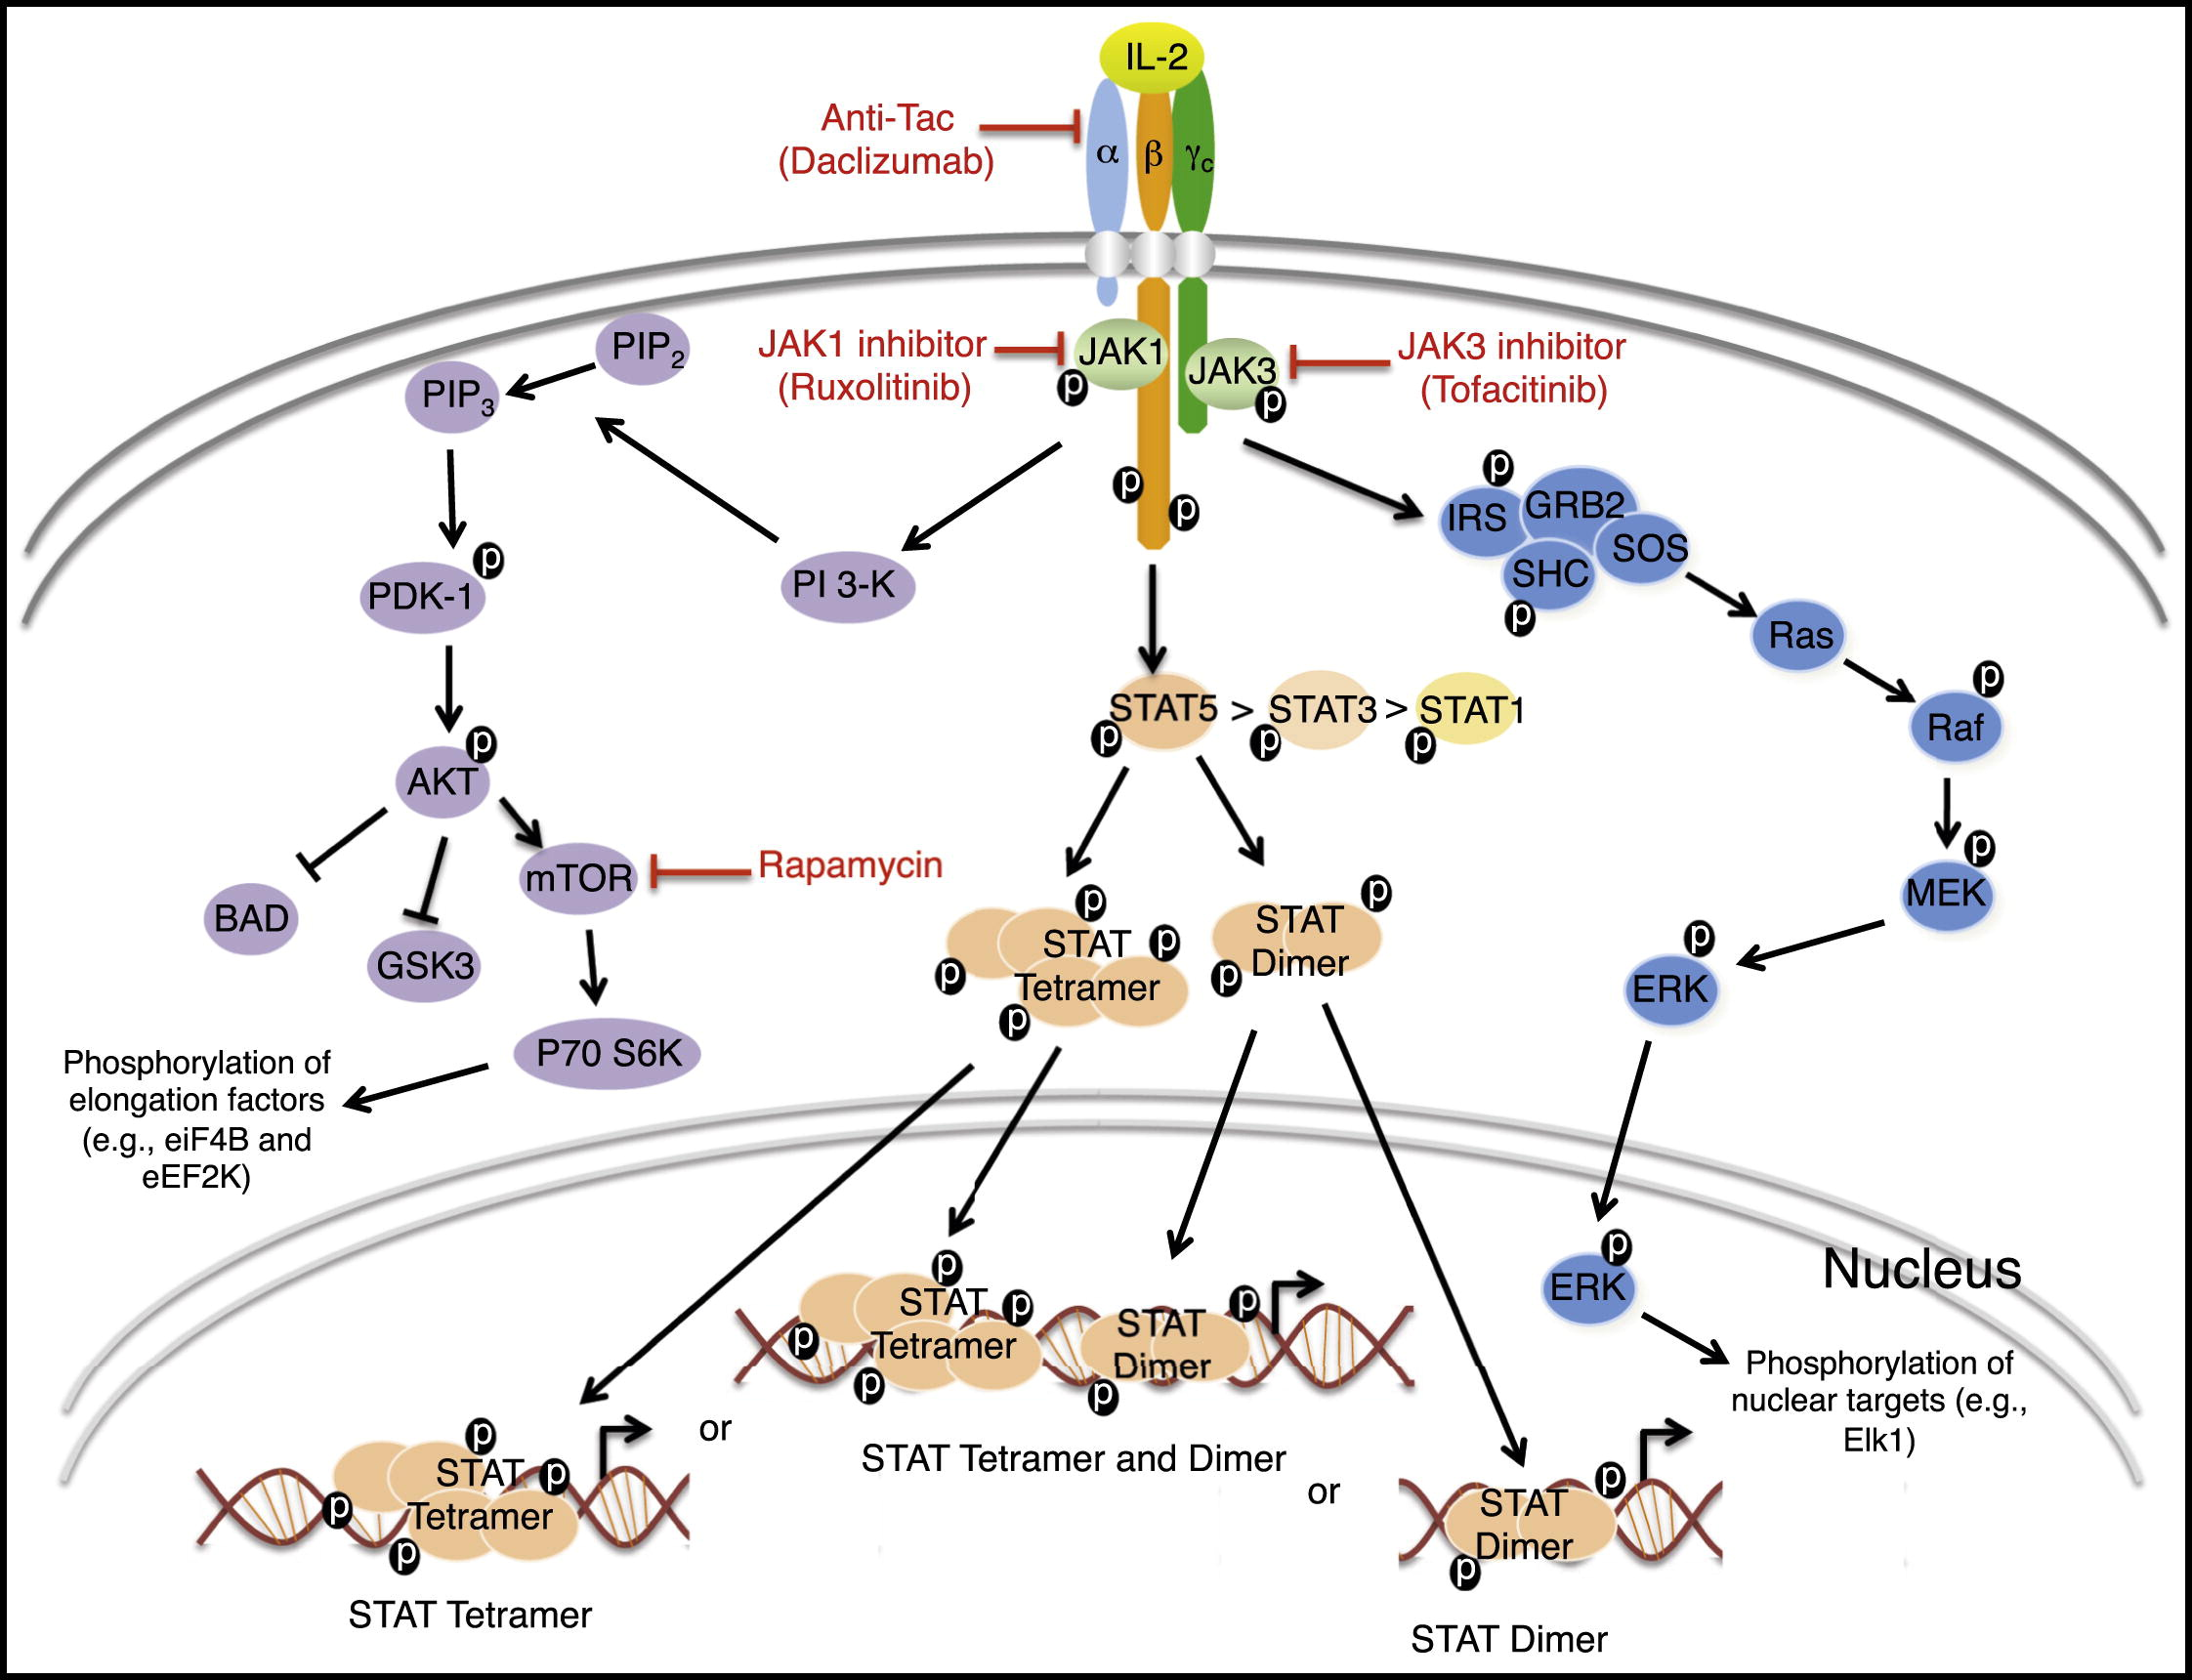
\includegraphics[scale=0.75]{IL2/figures/IL2-pathway.jpg}
\mycaption{figure:jones-2000}
{Schematic of major IL-2 signaling pathway (taken from \citet{Liao:2013jt}).}
{
\protein{CD25} is \protein{IL2RA}, the $\alpha$ subunit of the trimeric \cytokine{IL-2} receptor.
The $\alpha$ chain is the highest binding affinity receptor of the three chains.
STAT5 is phosphorylated to pSTAT5 and acts as a transcription factor.
%Schematic of Major IL-2 Signaling Pathways
%Shown is the activation of PI 3-K-AKT, JAK-STAT, and SHC-RAS-MAPK signaling pathways. Also shown are potential therapeutic points of control for IL-2 signaling, with anti-Tac (daclizumab), rapamycin, and JAK1 or JAK3 inhibitors being shown in red. The cartoon shows signaling by both STATs dimers and tetramers. The figure indicates that IL-2 activates more STAT5 than STAT3 and more STAT3 than STAT1. ERK refers to both ERK1 and ERK2. MEK refers to both MEK1 and MEK2.
}
\end{figure}

\citet{Long:2011hk} have reported that a \Gls{T1D} associated variant at \snp{rs1893217}
of the protein tyrosine phosphatase N2 gene (\gene{PTPN2}),
a negative regulator of the IL-2 pathway,
also correlates with lower STAT5 phosphorylation.
%show diminished ability to respond to \cytokine{IL-2}.
Furthermore, it is suspected that \cytokine{IL-2} production might be diminished in T1D since disease associated \gene{IL2RA} variants 
correlate with reduced CD25 levels 
and reduced \cytokine{IL-2} production
on activated CD69\positive CD4\positive memory T cells
after antigen stimulation \citep{Dendrou:2009dv}.
%with staphylococcal enterotoxin B 
%really?
Long-term reduced sensitivity to IL-2 also correlates with dimished maintenance 
of FOXP3 expression in the CD4\positive CD25\positive regulatory T-cells of type 1 diabetic subjects \citep{Long:2010ej}.
%Defects in IL-2R signaling contribute to diminished maintenance 
%IL-2 sensitivity drives IL-2 stimulation
%Preliminary data also suggests that the sensitivity to IL-2, measured in terms of pSTAT5 activation, may be also be reduced in the regulatory CD4+ T cells of newly diagnosed T1D patients.
%Furthermore it is also suspected that IL-2 production might be diminished in T1D
%since disease associated variants in the \emph{IL2RA} and \emph{PTPN2} genotypes correlate with reduced IL-2 production (reference?). 
Hence, these findings appear to consolidate the hypothesis that type 1 diabetics tend to have a reduced ability to respond to IL-2
in part due to genetic defects in \gene{PTPN2}, \gene{IL2RA} and possibly other gene variants involved in the IL-2 signalling pathway
%and that this decreased sensitivity is most noticeable in regulatory T cells
\citep{Long:2010ej,Long:2011hk,Long:2012ea}.
%The cell subsets are not always consistently defined across studies.
%Long:2010ej define Tregs as CD4+ CD25hi (FOXP3 not measured)
%Long:2011hk report that CD4+ CD45RO+
%nor is the definition of response to IL-2
%sometimes pSTAT5 MFI is measured, sometimes pSTAT5 pct positive, sometimes pSTAT5 fold change
These results are of great clinical relevance to us,
since our lab is currently conducting an
adaptive study of IL-2 dose on regulatory T cells in type 1 diabetes (\url{http://www.clinical-trials-type1-diabetes.com/}),
and to all researchers interested in low-dose IL-2 therapy to autoimmune diseases \citep{Koreth:2011kv,Saadoun:2011em}.

However some concerns have been raised with these studies.
One concern was that the Tregs discrimination was not particulary thorough.
%nor consistent
\citet{Long:2010ej} define Tregs based only on two markers CD4\positive CD25\positive whereas these cells are usually
also defined on CD127 and FOXP3.
Another a notable omission by \citet{Long:2010ej} was the lack of repeated samples to assess the within-individual variance
or reliability of the assay.
%Although \citet{Long:2011hk} do assess repeatability in 16 individuals, its not accounted for in the association test.
%clinical trials which
%treat type 1 diabetics with IL-2.
Hence, \contributor{Tony Cutler}, in our lab, set to find if he could replicate some of these findings in an independent cohort
using a more refined gating stategy by including the FOXP3 regulatory T cell marker,
%T1D leads to decrease sensitivity to IL-2 in similar sample size with 
as well as NK cell markers, CD3, CD8, and CD56,
%and the naive cell marker CD31,
to discover whether other potential cell subsets
are also sensitive to IL-2 (\Cref{table:IL2-panels}).
%and using repeated samples.

\paragraph{Samples and panels}

He selected 22 long-standing diabetics (6 males and 16 females, mean age 29) and 28 controls (mean age 27) from the Cambridge Bioresource,
as well as 30 newly diagnosed (20 males and 9 females, mean age 11.7) and 15 unaffected siblings (5 males and 12 females, mean age 12.3) from the \Gls{D-GAP} resource.  
%This was to determine if there was a difference between newly diagnosed and long-standing diabetics while controlling for age.
To guard from false positive association and non-reproducible results, 
it is important to ascertain the repeatability of these cell phenotypes before conducting any form of association study.
%Before proceeding with association testing of these cell phenotypes with T1D status or other covariates,
In order to test the repeatability, ten individuals were recalled for a second blood sample (\Cref{table:IL2-recalled-individuals}).
Hence a total of 52 cases and 43 controls, of which, 10 individuals (5 cases and 5 controls) from the Cambridge Bioresource were recalled to assess reproducibility
of the phenotypes.  

\begin{table}[ht]
\centering
\begin{tabular}{llll}
  \hline
Individual & status  & pch & number of days between visits \\
  \hline
1          & control & a   & 98 \\
2          & case    & b   & 140 \\
3          & control & c   & 167 \\
4          & control & d   & 98 \\
5          & case    & e   & 167 \\
6          & case    & f   & 112 \\
7          & control & g   & 112 \\
8          & case    & h   & 98 \\
9          & case    & i   & 120 \\
10         & control & j   & 140 \\
   \hline
\end{tabular}
\mycaption{table:IL2-recalled-individuals}
{Ten individuals recalled between 98 and 168 days later to assess stability of the cell phenotypes. }
{
pch is the plotting character used to refer to these individuals in plots later in this chapter.
}
\end{table}
%In order to test these hypotheses, we selected 21 long-standing diabetics and 30 controls from the Cambridge Bioresource,
%as well as  28 newly diagnosed and 14 unaffected siblings from DGAP.
%The nature of the resource allows more flexibility to recall patients of interest, i.e those with low IL-2 signalling potential, for more in depth analysis.
%To test this hypothesis, blood samples are taken from 21 type 1 diabetics and 30 healthy controls.  
Blood samples were prepared and analysed by flow cytometry on day of collection.
Each sample was split into four aliquots of \SI{500}{\micro\litre}.
The first aliquot was left unstimulated.
The remaining three were stimulated ex-vivo for 30 minutes at four 100-fold increasing doses
of proleukin (a polymer of \cytokine{IL-2}) at $0.1$, $10$ and \SI{1000}{\unit\per\milli\litre} respectively.
%\SI{1000}{\unit\per\micro\litre} respectively.
After a set stimulation time, the samples were fixed, permeabilised and stained, with different panels (\Cref{table:IL2-panels}), 
on a set of core markers, not expected to be affected by short-term proleukin stimulation,
CD4, CD25, CD45RA and FOXP3.
These were used to delineate different cell types, and the functional marker, pSTAT5
, a signalling protein of the IL-2 pathway phosphorylated on IL-2 stimulation (\Cref{figure:jones-2000}),
was used to measure IL-2 response.
Samples were analysed individually with flow cytometry, with all \gls{T1D} samples except for two run in parallel with healthy controls
to account for batch effects (\Cref{figure:IL2-sample-time}).
Samples were also matched for age and sex to allow for paired analysis.

%We address the following research questions relating to the pSTAT5 response in these samples:
%\begin{itemise}
  %%\item Can some individuals be classified as low/high responders?
  %\item In the cell subsets identified by manual gating, is the response to IL-2 associated with case-control status or any other covariate? 
  %\item Using automated methods, can we find other responsive cell subsets which are ignored by the manual gating?
%\end{itemise}
%Answering the first question will depend on the reproducibility of the response between cell-subsets within individuals,
%and we will see if, as in \Cref{chapter:il2ra}, normalisation can improve the reproducibility.

%Tony Cutler, Saleha Hassan, Marcin Pekalski will be involved in immune function assays.
%Louise Bell will be ethics liason.
%Statistical analysis will be carried out by a delegated member of the Statistics team.
%Demands on DIL infrastructure 
%Blood handling rooms, BD LSRII Fortessa machine.  
\begin{table}[h!]\footnotesize
  \centering
\begin{tabularx}{\textwidth}{lcccc}
\rowcolor{Gray}
Flurochrome       & T/NK cell panel & CD4 T cell panel & CD4/naive cell panel & NK cell panel \\
Alexa Fluor 488   & pSTAT5          & pSTAT5           & pSTAT5               & pSTAT5  \\
Alexa Fluor 700   & CD4             & CD4              & CD4                  & CD4     \\
APC               & CD25            & CD25             & CD25                 & CD25    \\
Pacific Blue      & CD56            & CD45RA           & CD45RA               & CD45RA  \\
PE YG             & FOXP3           & FOXP3            & FOXP3                & FOXP3   \\
PE-Cy7 YG         & CD45RA          &                  & CD31                 & CD56    \\
PerCP Cy5-5       & CD3             &                  &                      & \\
Qdot 605          & CD8             &                  &                      & \\
\hline
Number of samples & 10              & 95               & 12                   & 66 \\
%Number of samples & 13 & 96 &
\end{tabularx}
\mycaption{table:IL2-panels}
{Proleukin stimulation assay antibody-fluorochrome panels.}
{
The fluorochrome-antibody panels used in IL-2 stimulation.
The panel used on the majority of samples was the CD4 T cell panel, used to disriminate
effector and regulatory naive and memory T cells.
The T/NK cell panel, which contains the most markers, was only ran on a subset of 26 samples.
}
\end{table}
%CD14-CD19-CD3-CD45RA-CD56-HLA-DR-PSTAT5
%1
%CD19-CD25-CD27-CD3-CD45RA-CD56-CD8-PSTAT5
%1
%CD19-CD25-CD27-CD3-CTLA4-PSTAT5
%1
%CD19-CD25-CD27-CD3-ISO-PSTAT5
%1
%CD25-CD31-CD4-CD45RA-FOXP3-PSTAT5
%5
%CD25-CD3-CD4-CD45RA-CD56-CD8-CD8-PSTAT5
%1
%CD25-CD3-CD4-CD45RA-CD56-CD8-FOXP3-PSTAT5
%13
%CD25-CD3-CD4-CD45RA-CD56-CD8-PSTAT5
%48
%CD25-CD3-CD4-CD45RA-CD56-FOXP3-PSTAT5
%37
%CD25-CD4-CD45RA-CD56-FOXP3-PSTAT5
%5
%CD25-CD4-CD45RA-FOXP3-KI67-PSTAT5
%1
%CD25-CD4-CD45RA-FOXP3-PSTAT5
%50
%
%\begin{figure}
%\centering
%\includegraphics[scale=.5] {flowdatasets/figures/il2-stimulation-samples-time.pdf}
%\mycaption{figure:IL2-sample-time} 
%{ Days on which samples are processed. }
%{
  %To account for day of analysis effect in the case-control association testing,
  %at least one healthy control sample and one type 1 diabetic sample were analysed per day.
%}
%\end{figure}

\myfigure{scale=.5}{IL2-sample-time} 
{ Number of cases and controls analysed per day. }
{
  To account for batch effects in the case-control association testing,
  Tony Cutler aimed to analyse, when possible,
  at least one healthy control sample and one type 1 diabetic sample per day.
  %However on some days the number of cases and controls did not match.
  On two days, 2012-09-04 and 2012-10-25, no matching controls were ran.
}


\section{Cell Phenotypes Identified by Manual Analysis}

In the preliminary manual analysis using FlowJo, \contributor{Tony Cutler},
%The pSTAT5 distribution was measured in effector and regulatory naive and memory T cell populations (Figure~\ref{figure:tony-cd4-gating}).
gated four CD4\positive lymphocyte subsets (\Cref{figure:tony-cd4-gating}):
\begin{itemise}
  \item memory effector
  \item memory treg
  \item naive effector
  \item naive treg
\end{itemise}
%\begin{figure}[h]
    %\centering
    %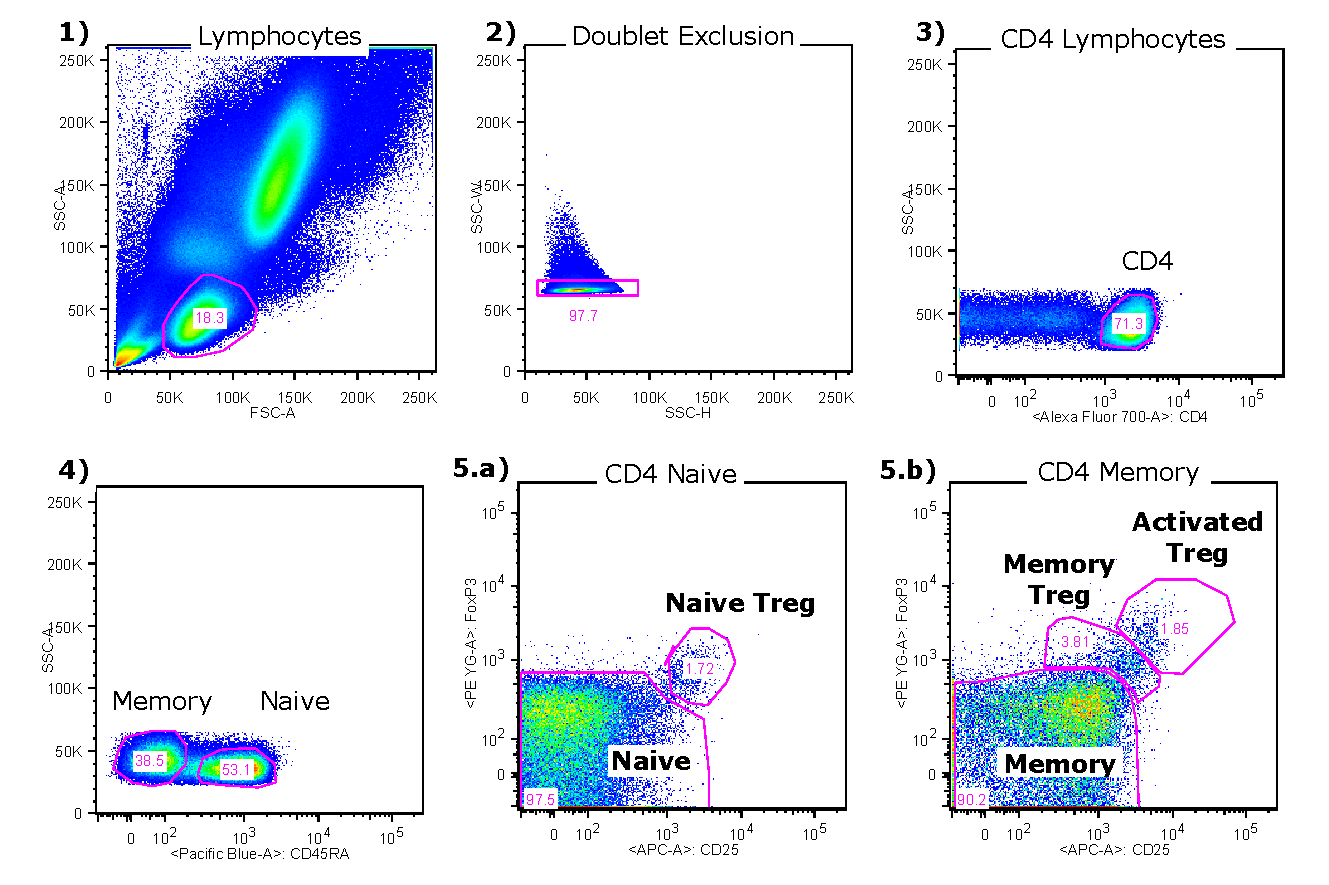
\includegraphics[scale=.75]{IL2/figures/tony-cd4-gating.pdf}
    %\caption{  \label{figure:tony-cd4-gating} Manual gating conducted by \contributor{Tony Cutler} to identify:
    %conventional and regulatory naive and memory T cells as well as activated regulatory T cells.
    %}
%\end{figure}
% 
%\hspace{-2cm}
\begin{figure}[h]
\centering
%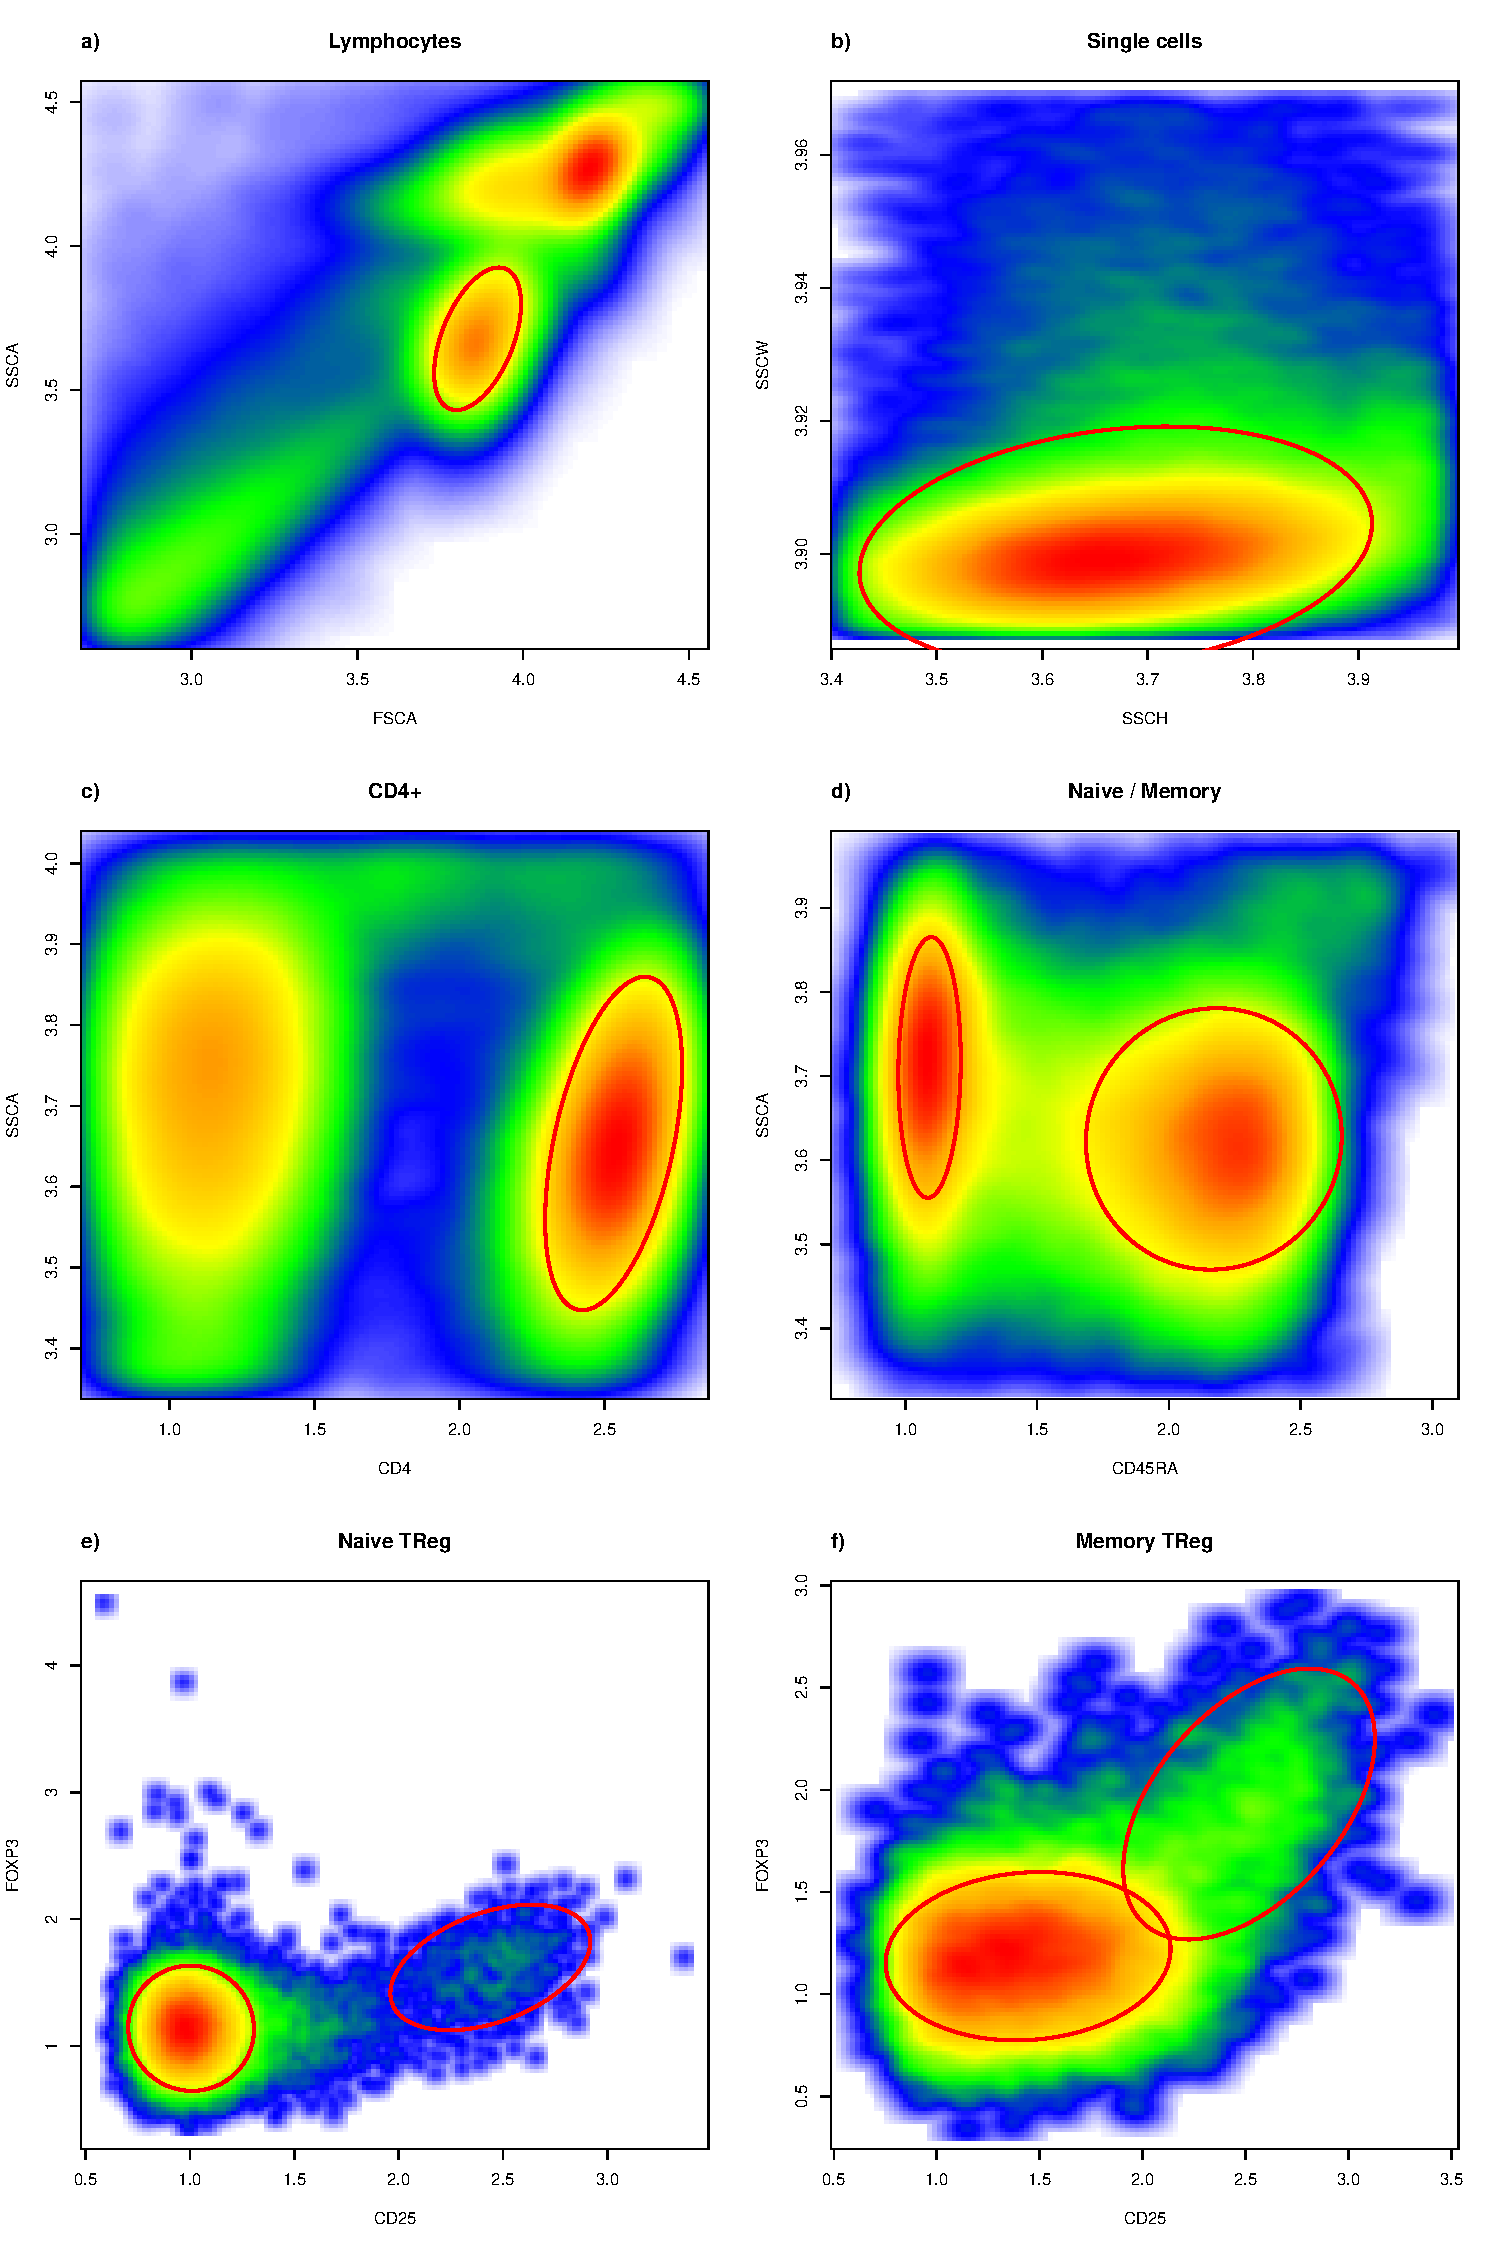
\includegraphics[scale=.5]{figures/manual-gating.pdf}
%\begin{subfigure}[b]{.4\textwidth}
%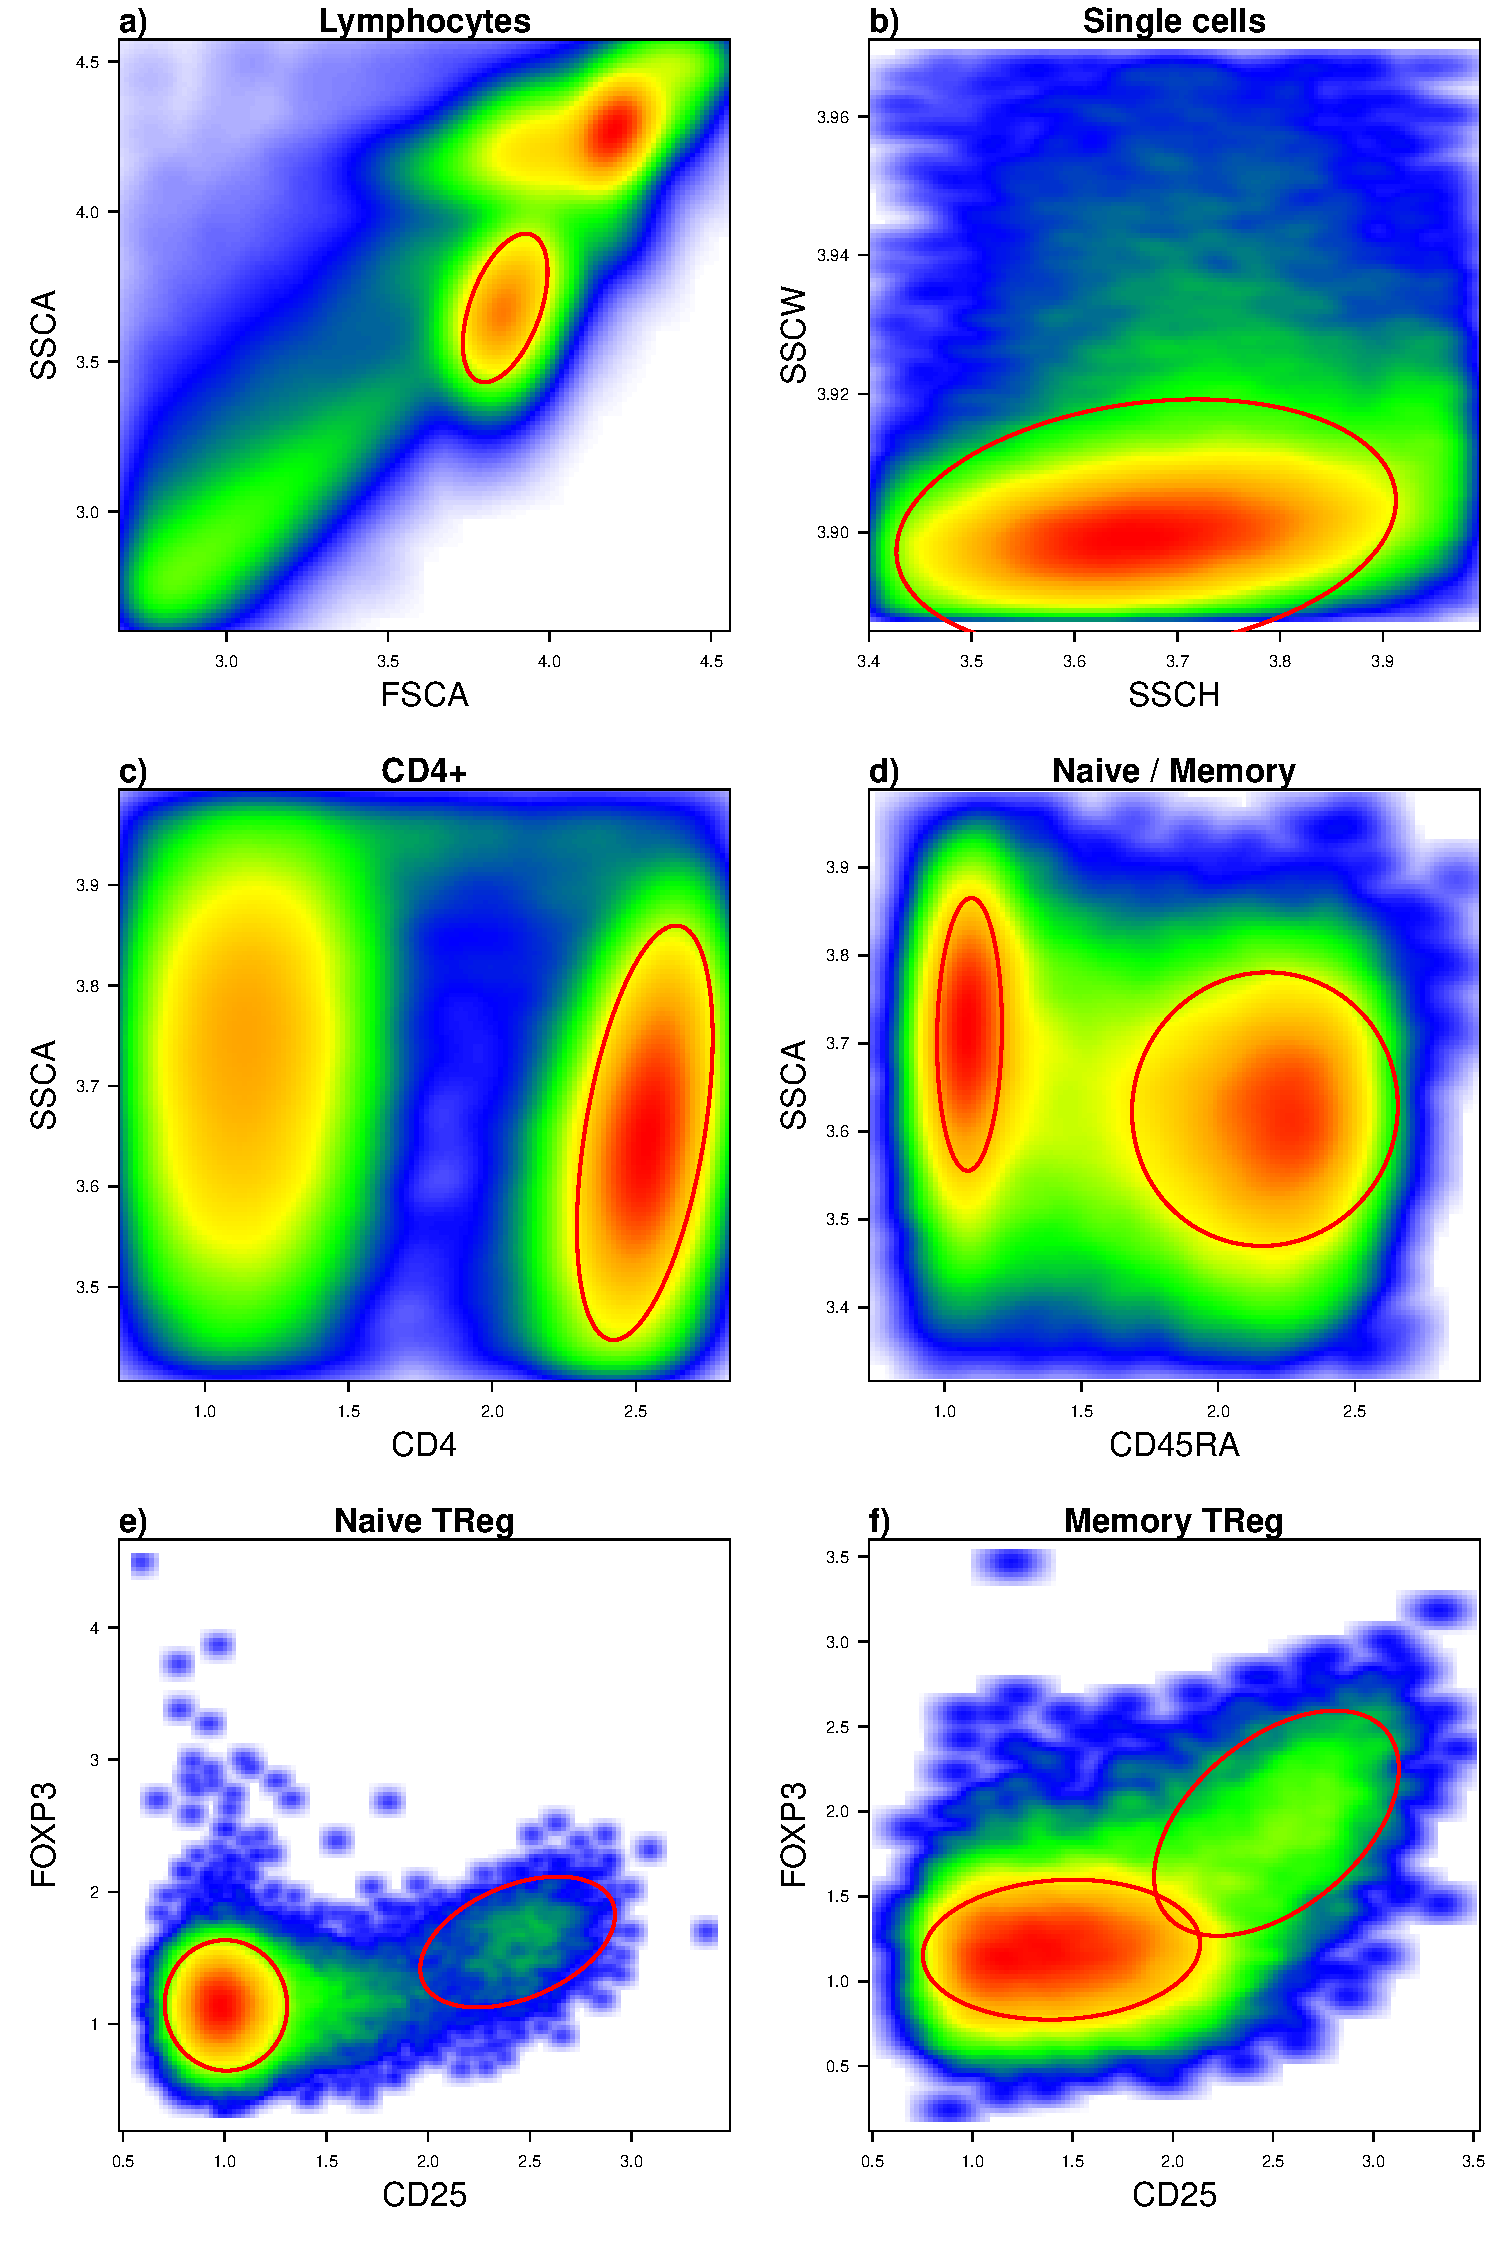
\includegraphics[scale=.25]{IL2/figures/manual-gating-CB00165D_0U_2012-11-29.pdf}
  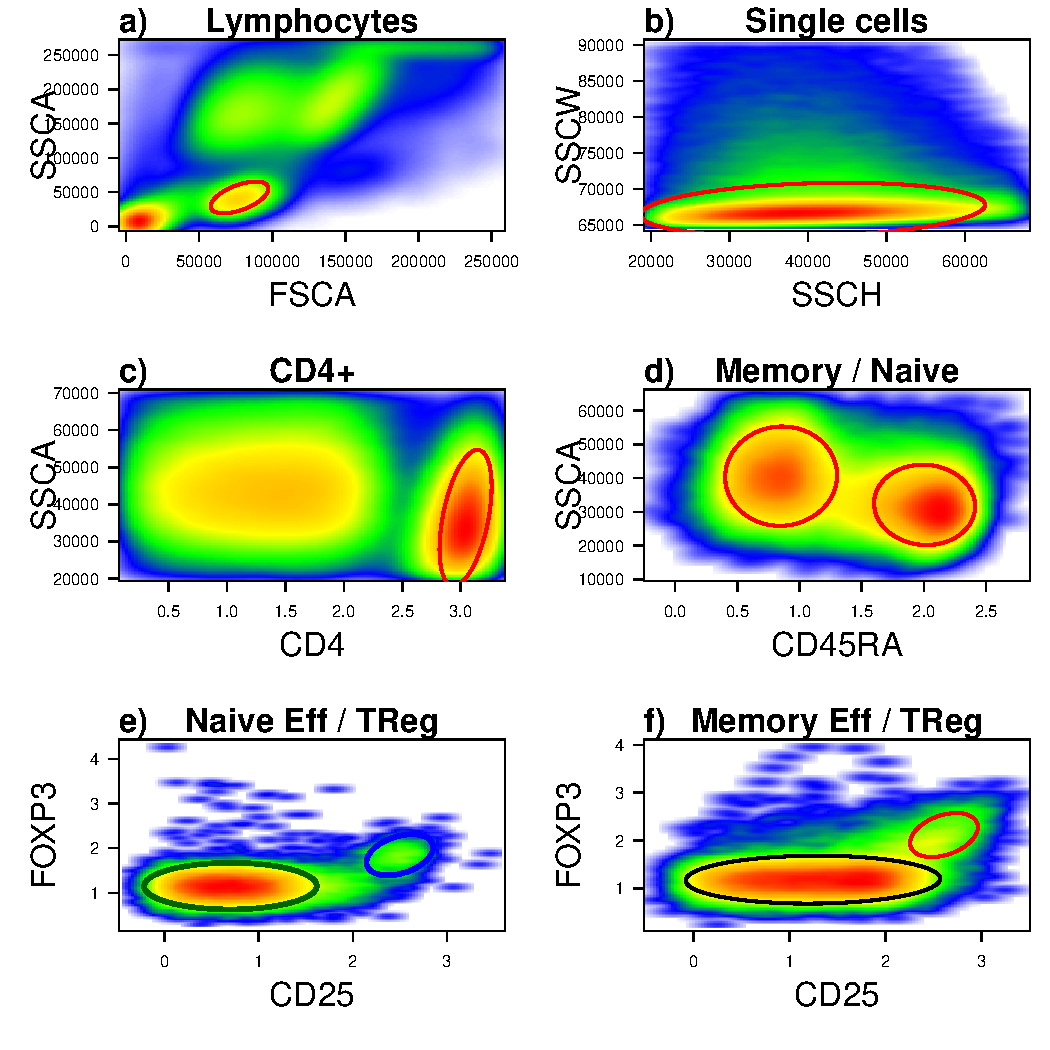
\includegraphics[scale=.75]{IL2/figures/CB00366X_2012-11-07.pdf}
%\caption{Resting sample.}
%\end{subfigure}
%\begin{subfigure}[b]{.4\textwidth}
%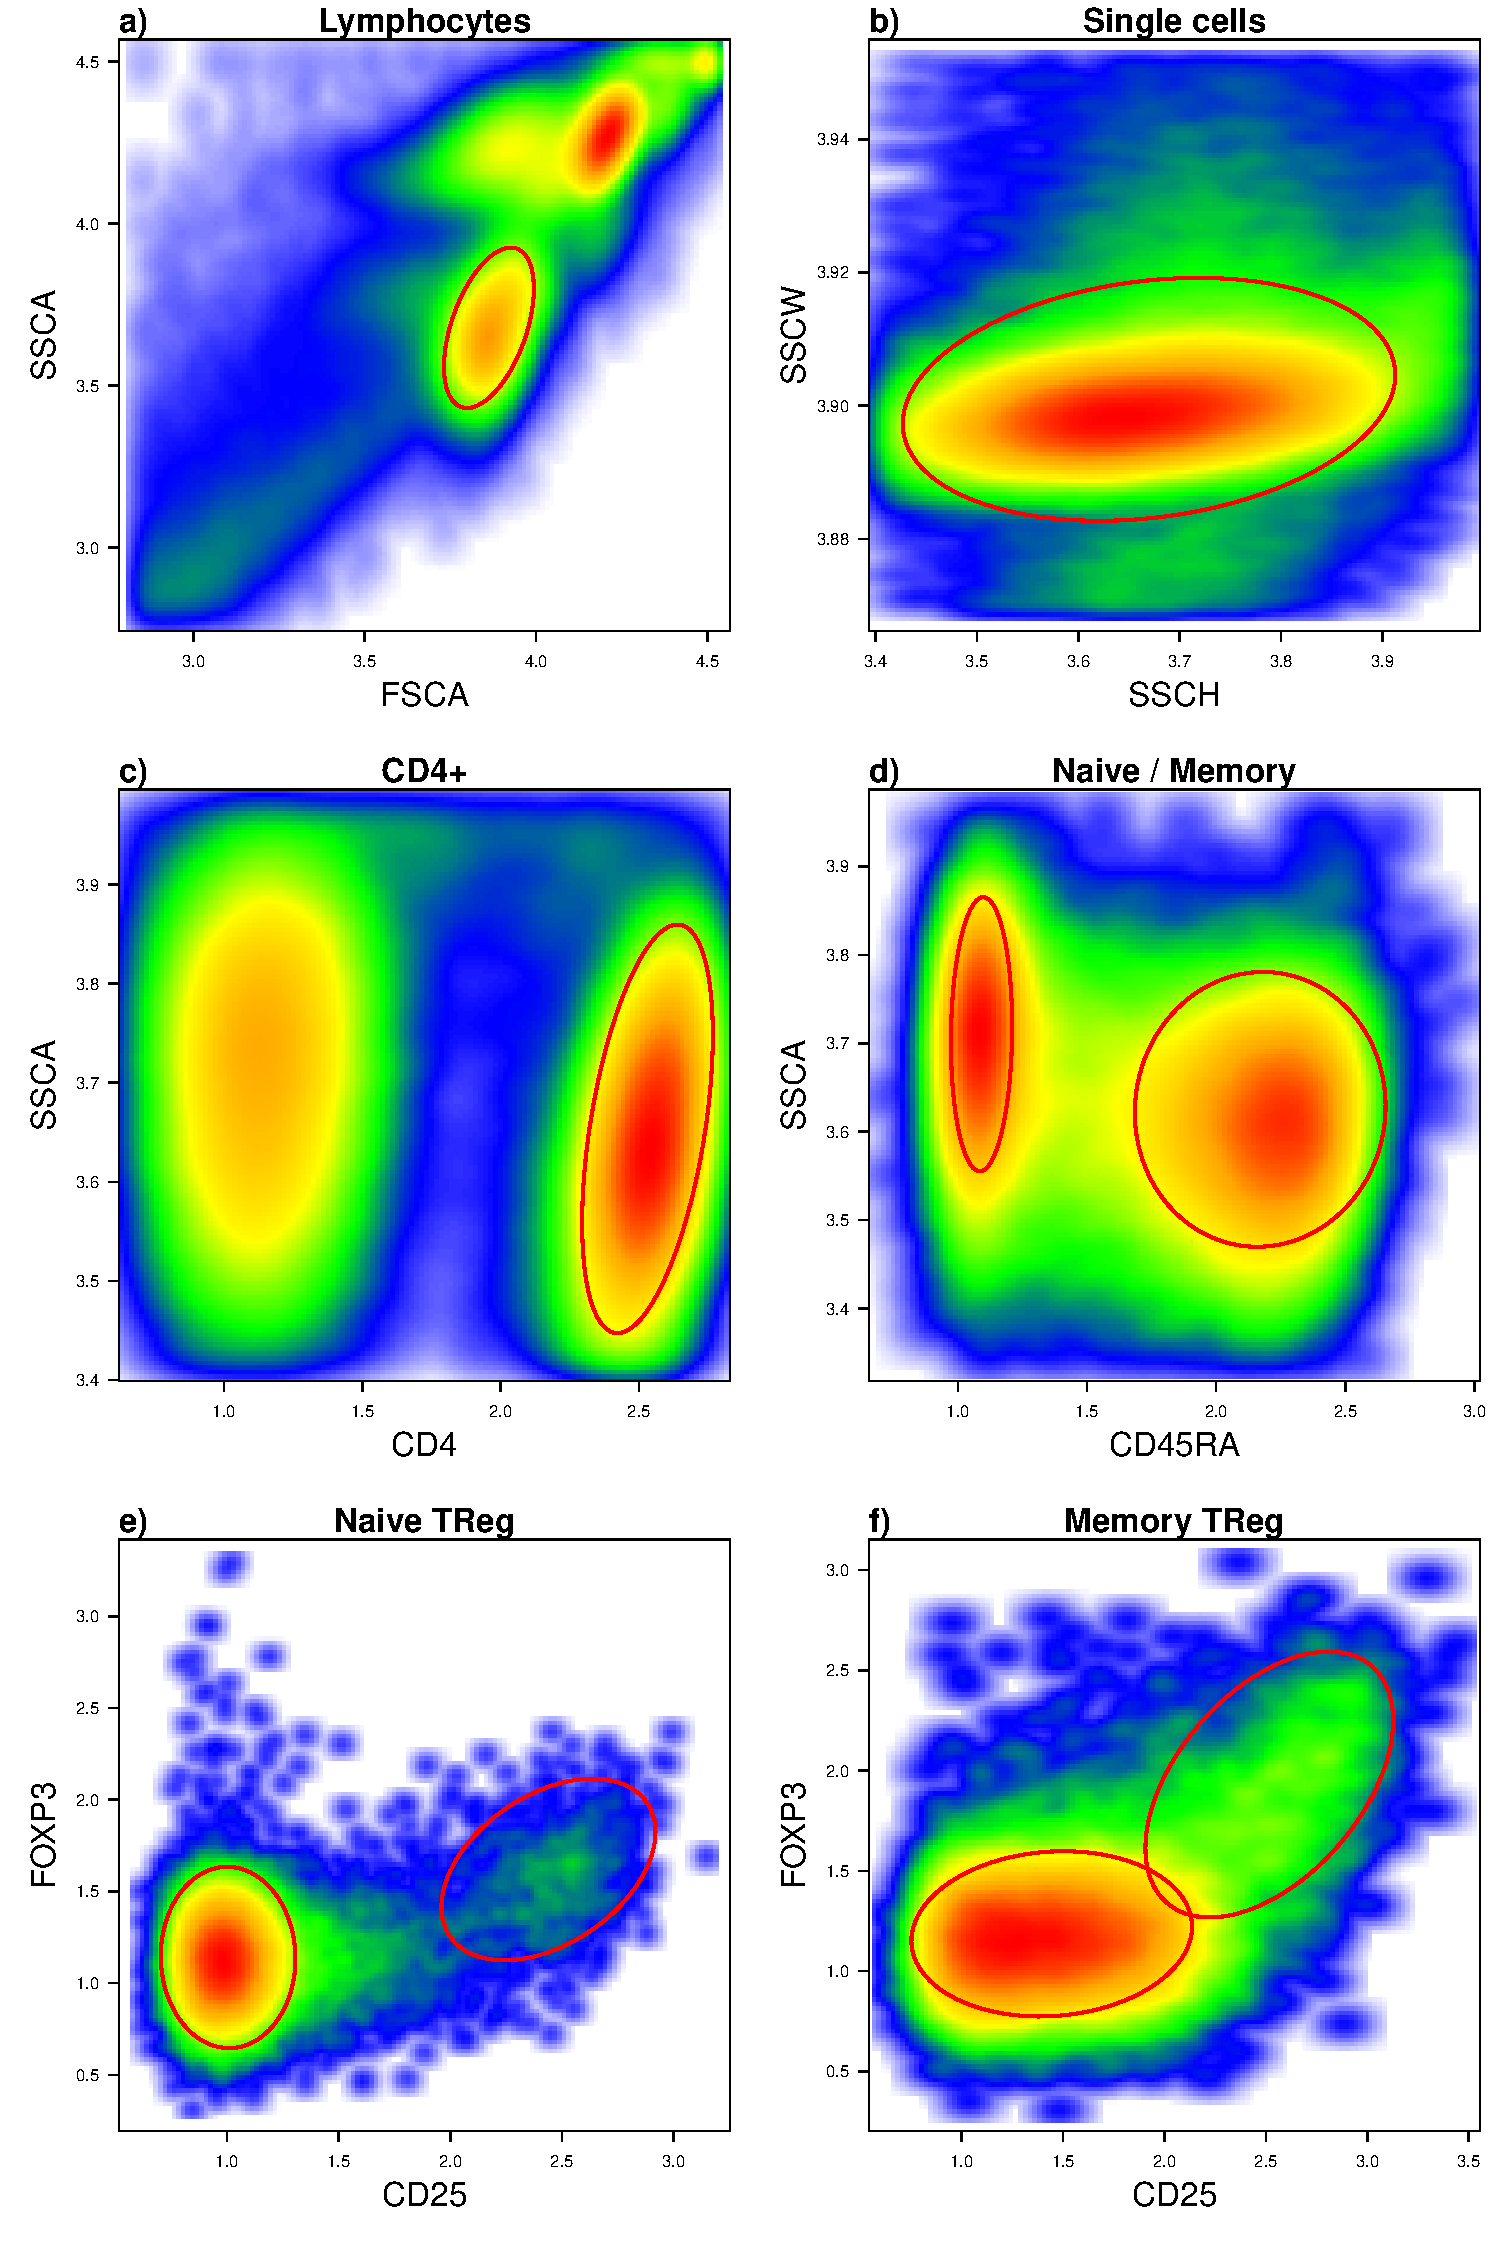
\includegraphics[scale=.25]{IL2/figures/manual-gating-CB00165D_01U_2012-11-29.pdf}
%\caption{Stimulated at 0.1 units of proleukin.}
%\end{subfigure}
%\begin{subfigure}[b]{.4\textwidth}
%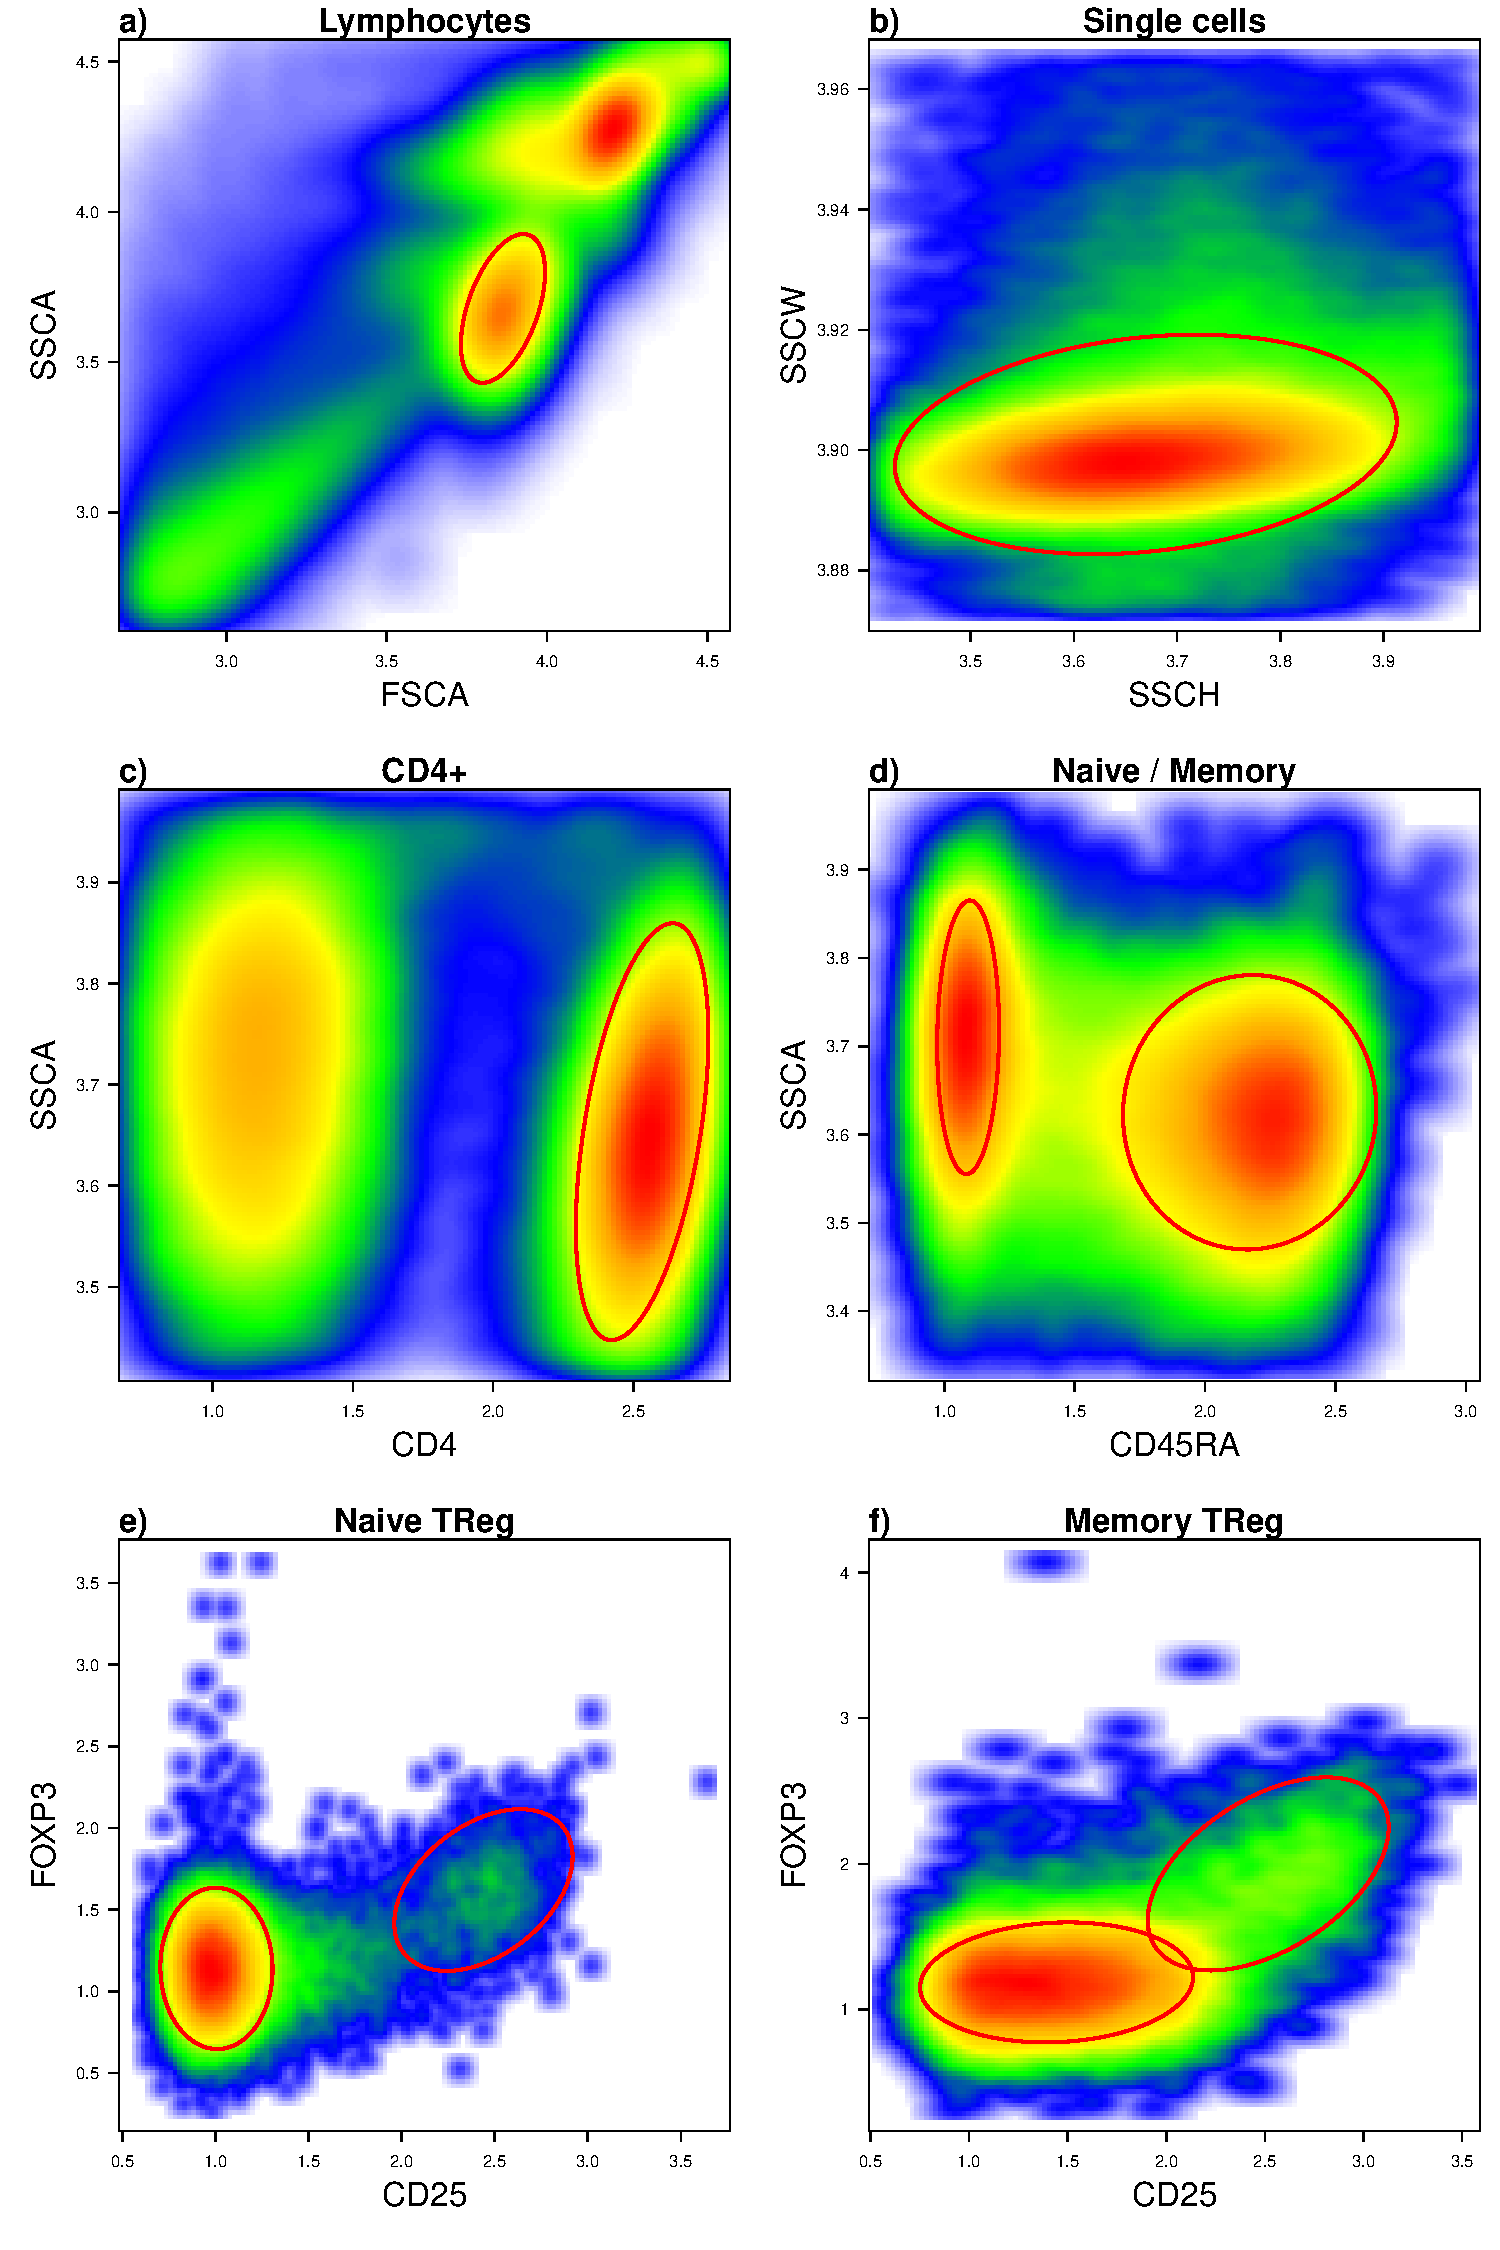
\includegraphics[scale=.25]{IL2/figures/manual-gating-CB00165D_10U_2012-11-29.pdf}
%\caption{Stimulated at 10 units of proleukin.}
%\end{subfigure}
%\begin{subfigure}[b]{.4\textwidth}
%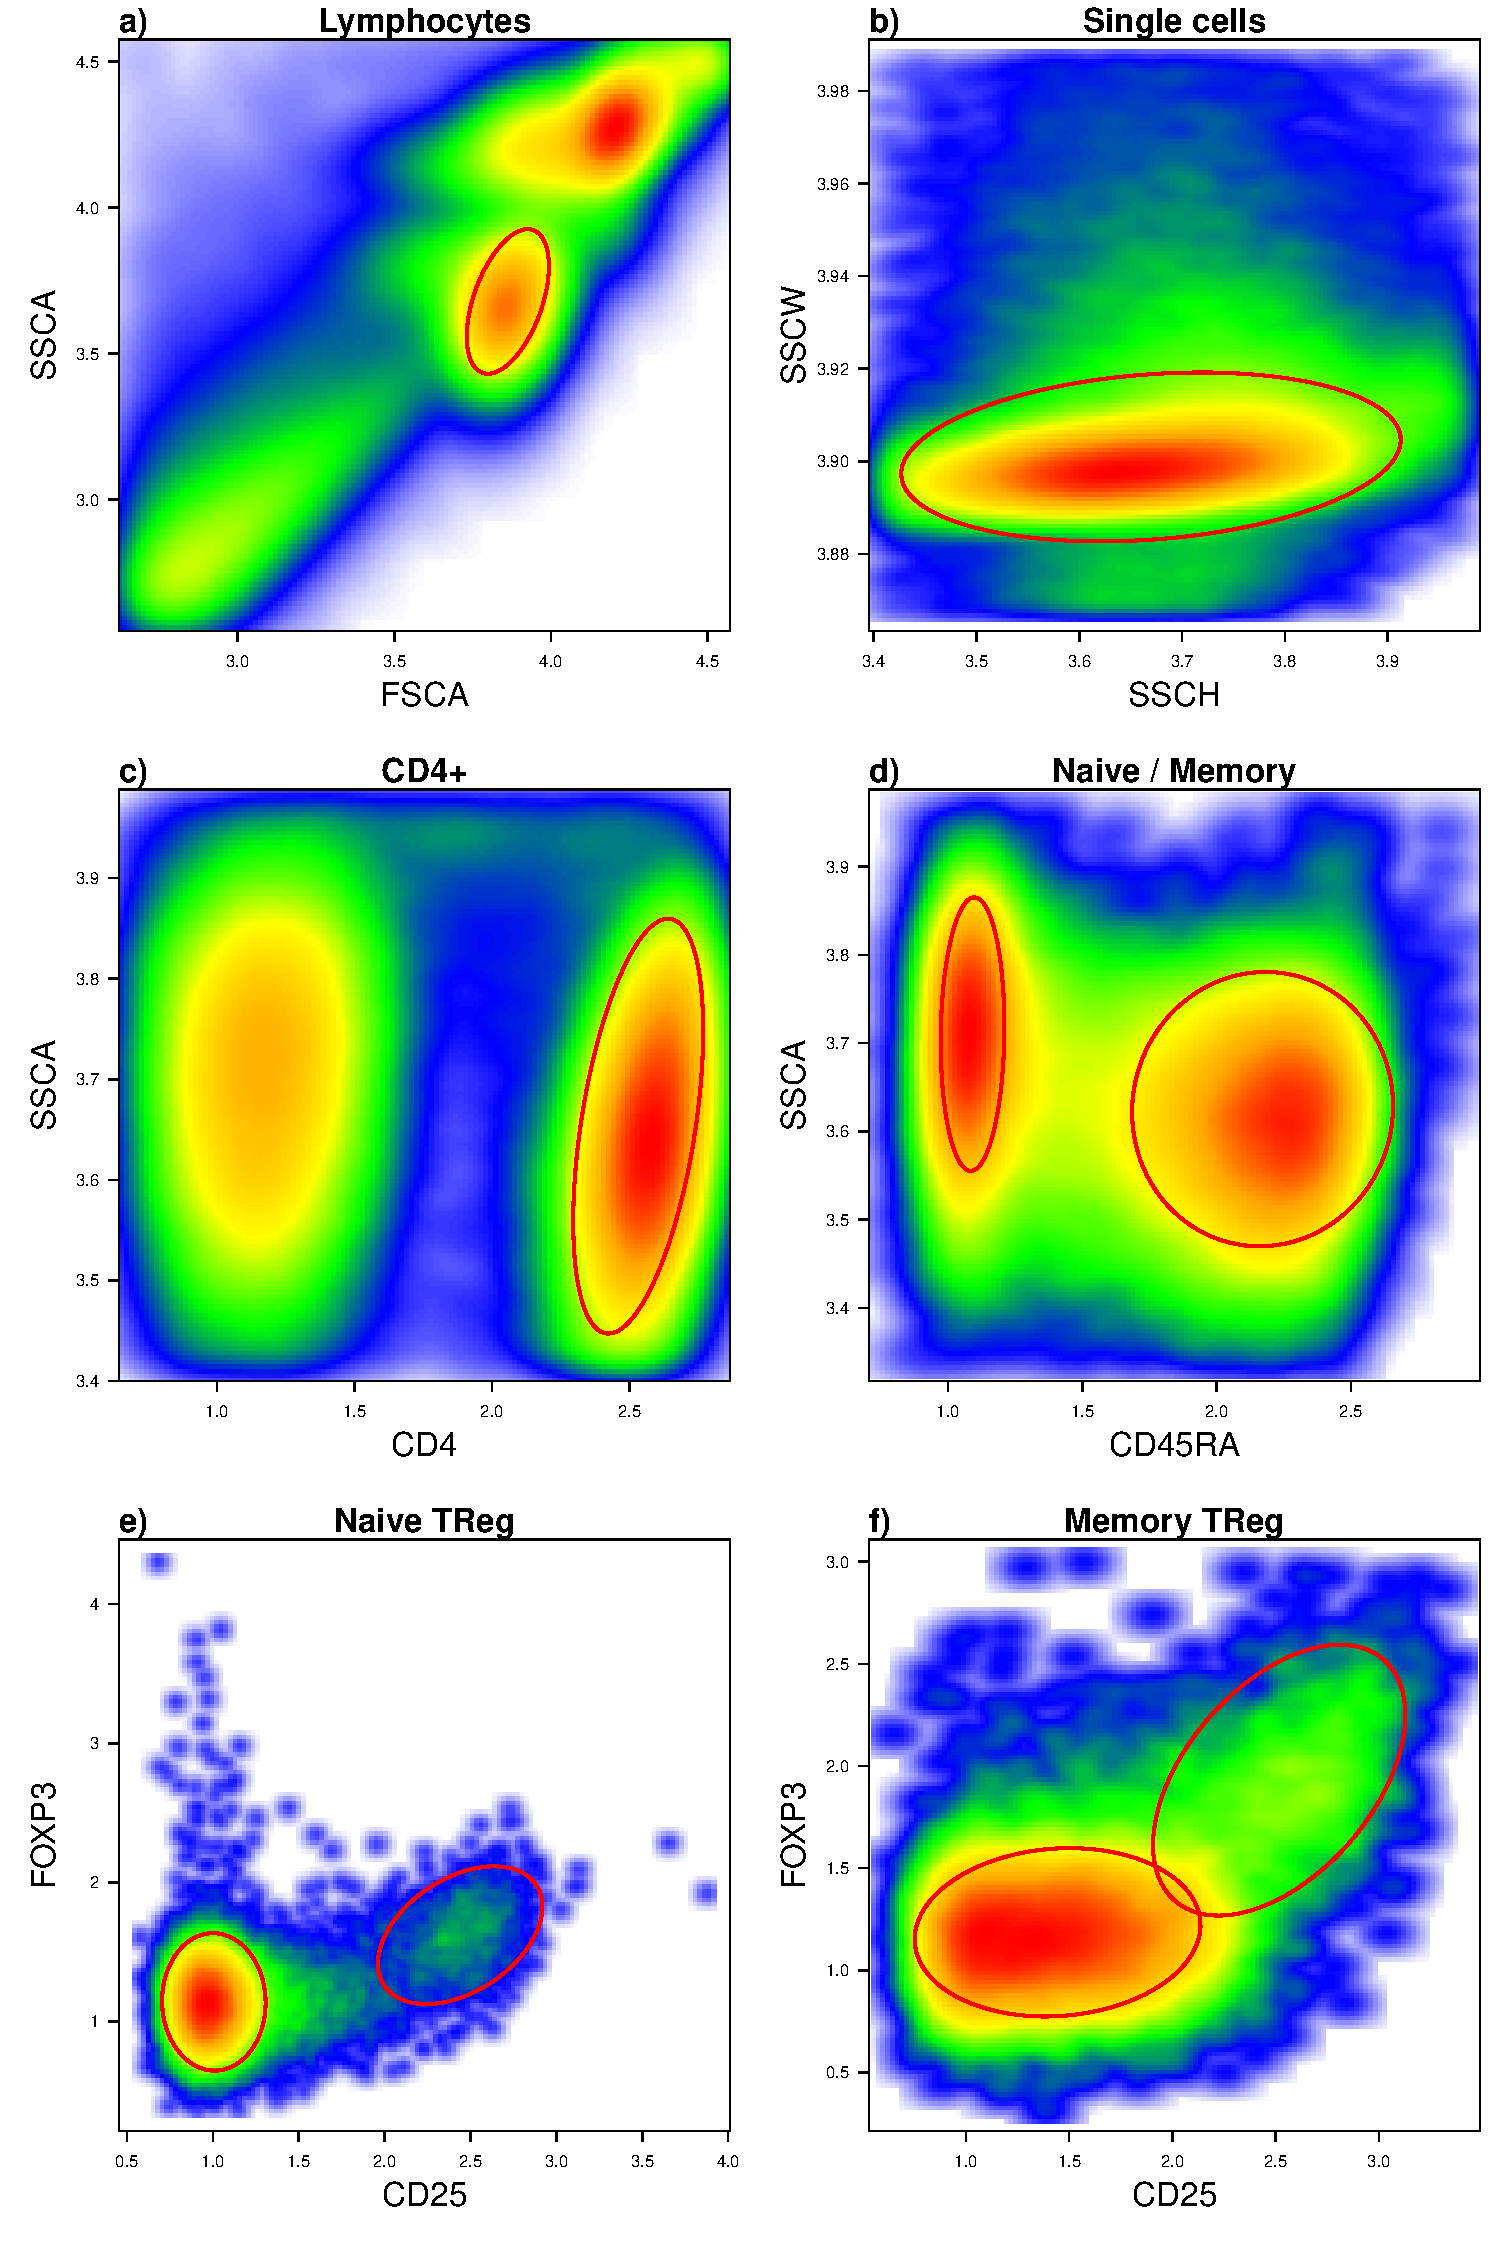
\includegraphics[scale=.25]{IL2/figures/manual-gating-CB00165D_1000U_2012-11-29.pdf}
%\caption{Stimulated at 1000 units of proleukin.}
%\end{subfigure}
\mycaption{figure:tony-cd4-gating}
{Gates applied across doses.}
{
Manual gating conducted using FlowJo by \contributor{Tony Cutler} to identify
naive effector (green ellipse) and regulatory T cells (blue ellipse) (e)
and memory effector (black ellipse) and regulatory T cells (red ellipse) (f).
%The same gates can be applied across doses (i, ii, ,iii, iv).
}
\end{figure}
Within each lymphocyte subset, the pSTAT5 distribution was measured, in each of the four samples stimulated at an increasing proleukin dose
(\Cref{figure:dose-effect-pstat5-cellsubsets}).  
As expected, the pSTAT5 distribution shifts progressively right for higher doses of proleukin, as more STAT5 is phosphorylated.
Of the four subsets, the most sensitive cells to proleukin are the smaller memory and naive regulatory T cell subsets (\Cref{figure:dose-effect-pstat5-cellsubsets} b and d),
then the memory effectors (\Cref{figure:dose-effect-pstat5-cellsubsets} a) and finally the naive effectors (\Cref{figure:dose-effect-pstat5-cellsubsets} c).
This correlates with the level of \protein{CD25} expressed by these cells.

%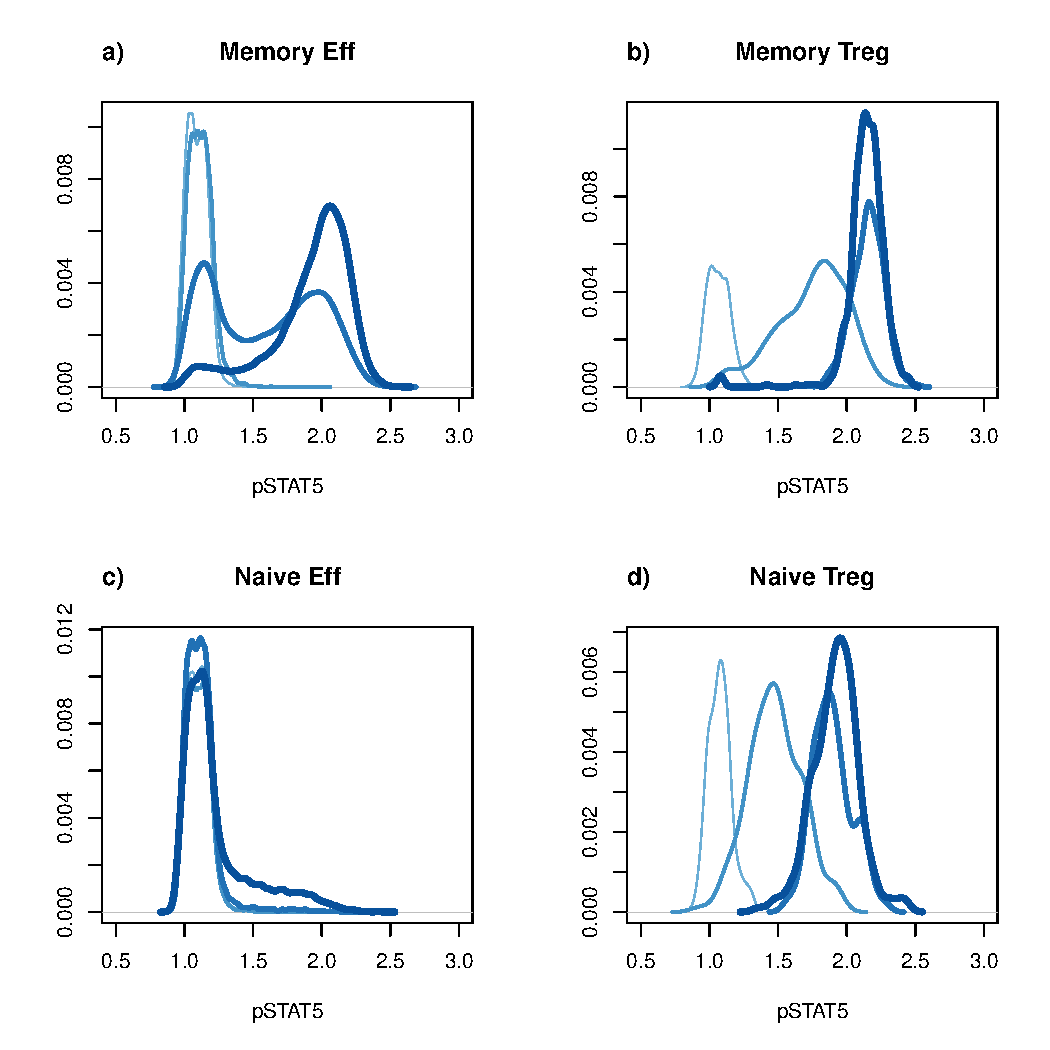
\includegraphics[scale=.45]{IL2/figures/dose-effect-pstat5-cellsubsets-density.pdf}
%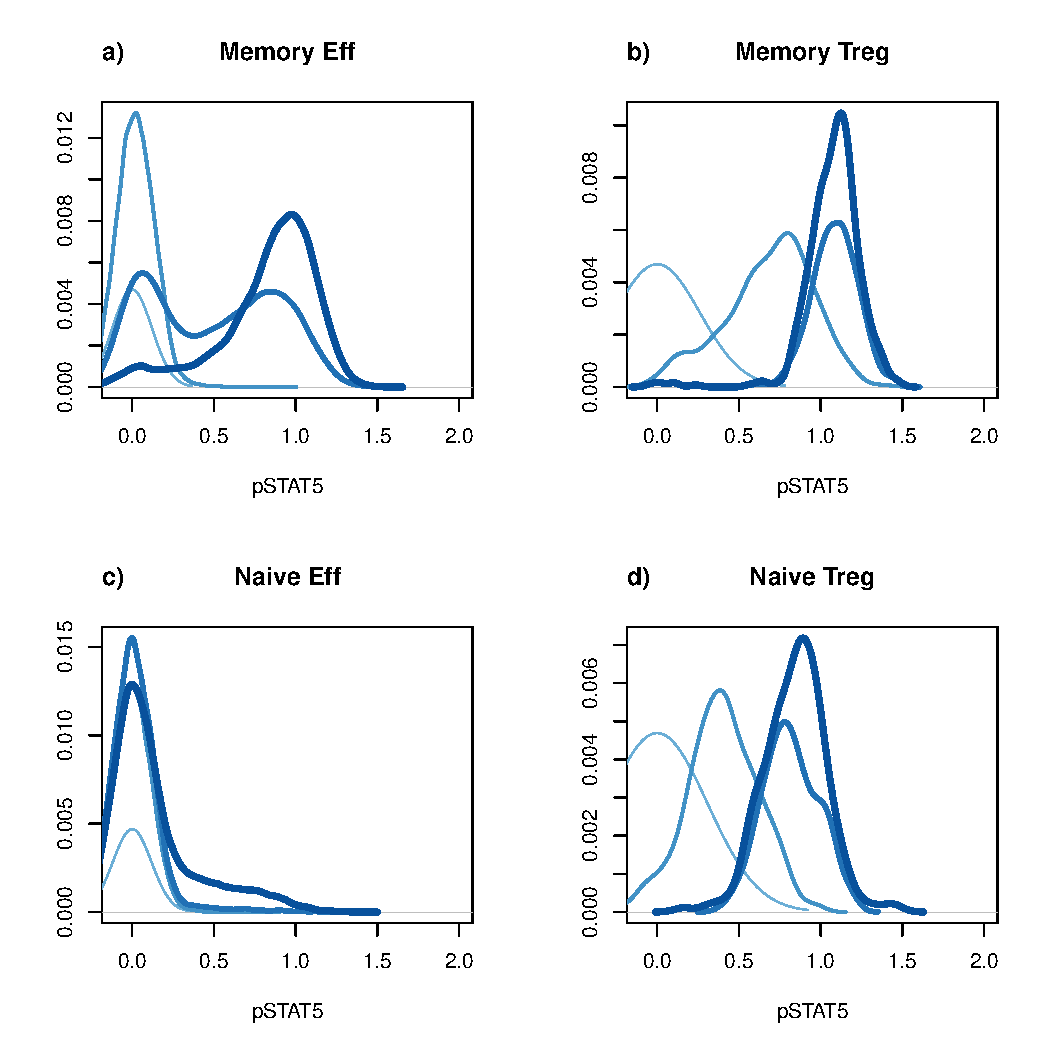
\includegraphics[scale=.45]{IL2/figures/dose-effect-pstat5-cellsubsets-density-baseline.pdf}
%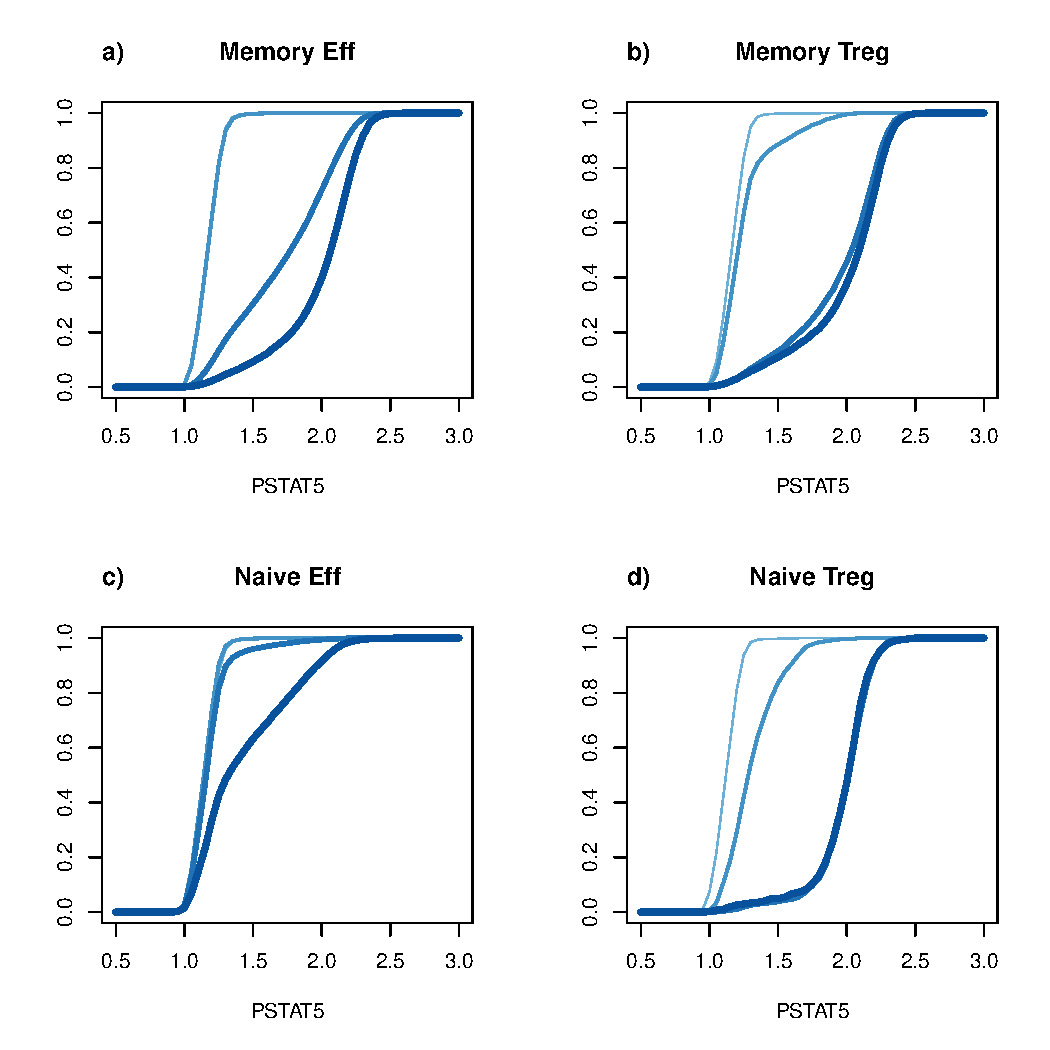
\includegraphics[scale=.45]{figures/dose-effect-pstat5-cellsubsets-ecdf-joined.pdf}
\myfigure{scale=.6}
%individual g
{dose-effect-pstat5-cellsubsets-density}
{ Distribution pSTAT5 in the manually gated cell subsets in the sample manually gated in \Cref{figure:tony-cd4-gating}. }
{
The thickness of the lines is representative of the four increasing doses of proleukin (0, 0.1, 10 and 1000 units).
The dose-response is most striking in the smaller Treg subsets with higher CD25 (b and d).
The dashed vertical line represents the 99th percentile of the pSTAT5 distribution in the resting sample,
which is used to define the pSTAT5\positive threshold.
}

Next \contributor{Tony Cutler}, assessed the repeatability of the pSTAT5 response by measuring the pSTAT5 \gls{MFI}
for each individual subset of lymphocytes tested.
However, this cell phenotype was poorly reproducible, since the location of the peaks was not stable across days as illustrated
by the sample shown in \Cref{figure:dose-effect-pstat5-cellsubsets-density-repeatability}.
%Furthermore, the \gls{MFI} is not a representative metric for bimodal distributions 
%However, one issue is that pSTAT5 MFI is not very representative for very bimodal or skewed distributions such
%as the memory effectors in \Cref{figure:dose-effect-pstat5-cellsubsets}.
%Also the resting pSTAT5, which represents the baseline pSTAT5, of the same cell subset may not be constant across days.  
%To address these issues, the percent of pSTAT5\positive cells was also assessed.
\myfigure{scale=.6}
%individual g
{dose-effect-pstat5-cellsubsets-density-repeatability}
{ pSTAT5 distribution in an individual on visit one (black) and visit two (red) clearly shows that pSTAT5 distribution is not stable across days in the four cell
subsets. }
{
In black, the pSTAT distribution on visit one and in red, on visit two.
%The thickness of the line represents the proleukin dose at which the sample was stimulated (0, 0.1, 10 and 1000 units).
The thinner lines are from the resting sample whereas the thicker lines are from the sample stimulated at 1000 units.
The vertical lines represent the pSTAT5\positive threshold set at the $99^{th}$ percentile of the pSTAT5 distribution in the resting sample.
}
This motivated \contributor{Tony Cutler} to instead use a threshold approach to define the ratio of cells which are pSTAT5\positive.
An idea similar to that applied in \Cref{chapter:il2ra} to define naive cells as CD25\positive.
%but the threshold is defined using the unstimulated sample rather than beads. 
%It is a good approach to use when the number of cells is small
%and is commonly used in populations with high CV.
However, here an internal threshold was used, namely
the threshold was defined to be the 99th percentile of the pSTAT5 distribution in the resting cell subset per sample.
Thus each each sample and cell subset had its own pSTAT5\positive threshold.
He presented his results in six of the ten repeated individuals for the four stimulated cell subsets,
memory effector (\Cref{figure:tony-memory-eff}),
memory regulatory T cells (\Cref{figure:tony-memory-treg}),
naive effector (\Cref{figure:tony-naive-eff})
and naive regulatory T cells (\Cref{figure:tony-naive-treg}).
For memory and naive Tregs (\Cref{figure:tony-memory-treg,figure:tony-naive-treg}), at the highest 1000 units dose,
practically all memory and naive tregs are pSTAT5\positive.
However, these cell populations show a significant response already at the lowest 0.1 units dose of proleukin.
Based on this observation, \contributor{Tony Cutler} selected the
memory and naive Treg pSTAT5 cell phenotype to be the percentage of pSTAT5\positive cells at the 0.1 units dose.
On the other hand, since memory effectors are less reponsive, 10 units was chosen as the representative dose.
For naive effectors, the least reponsive of the four cell subsets considered, the repeatability was assessed at the 1000 unit dose.
Tony assessed the repeatability with the coefficient of determination:
%instead of using the square of the Pearson correlation: 
\[
  R^2 = 1 - \frac{\sum_{i=1}^N (x_{i1}-x_{i2})^2}{\sum_{i=1}^N (x_{i1}-\overline{x_1})^2}
\]
where $x_{i1}$ is the phenotype of $i^{th}$ individual on the first day and $x_{i2}$
is the phenotype of the $i^{th}$ individual on the second day.
The coefficient of determination can take negative values if the correlation between $x_{i1}$ and $x_{i2}$ is very low.
Contrary to the Pearson correlation, used in the previous chapter, the coefficient of determination is sensitive to linear transforms.
%this is not correct because it's not symmetric
Even when using the percent of pSTAT5\positive cell phenotype,
the overall reproducibility across the four cell subsets was still poor,
with the more sensitive and smaller cell subsets,
naive and memory Tregs showing the worst correlation ($R^2=-0.16$ and $R^2=-0.82$), memory effectors showing slightly better correlation ($R^2=0.021$)
and finally the less responsive naive effectors showing good correlation ($R^2=0.7728$) (\Cref{figure:tony-repeatability}).
Tony then went on to test association with type 1 diabetes using a two-tailed paired t-test of 20 cases matched with 20 controls analysed on the same
day (\Cref{figure:tony-t1d-association}).
%how did he deal with repeats?
He also tested for association with \gene{IL2RA} SNP \snp{rs12722495}, and the
\gene{PTPN2} SNPs \snp{rs45450798} and \snp{rs478582} (plots not shown).
No significant association was detected either with disease nor with genotype.

\myfigure{scale=.5}
{tony-memory-eff}
{ The percent of pSTAT5\positive cells increases with proleukin dose in memory effectors,
but the measured response is not consistently repeatable (f, g). }
{
  Plot produced by Tony Cutler.
}
\myfigure{scale=.5}
{tony-memory-treg}
{ The percent of pSTAT5\positive cells increases with proleukin dose in memory tregs. }
{
  Plot produced by Tony Cutler.
  While at the highest proleukin dose of 10 and 1000 units, all memory tregs are consistently pSTAT5\positive,
  there is more discrepancy at the low dose of 0.1 units.
}
\myfigure{scale=.5}
{tony-naive-eff}
{ The percent pSTAT5\positive cells increases with proleukin dose in naive effectors. }
{
  Plot produced by Tony Cutler.
  Only \pct{40} of the naive effector cells are pSTAT5\positive even at the highest 1000 unit proleukin dose.
}
\myfigure{scale=.5}
{tony-naive-treg}
{ The percent pSTAT5\positive cells increases with proleukin dose in naive tregs. }
{
  Plot produced by Tony Cutler.
  While at the highest proleukin doses of 10 and 1000 units, all naive tregs are consistently pSTAT5\positive,
  there is more discrepancy at the low dose of 0.1 units.
}
\myfigure{scale=.75}
{tony-repeatability}
{ Repeatability in six individuals }
{
  Plot produced by Tony Cutler.
  The repeatability of the percent of cells which are pSTAT5\positive is assessed in effector memory and naive at the 10U and 1000U dose
  respectively, and in memory and naive regulatory T cells at the 0.1U dose.
  While the repeatability in the naive effector subset was good ($R^2=0.7728$), the repeatability in the other cell subsets is poor
  (memory effectors $R^2=0.021$, naive tregs $R^2=-0.16$ and memory tregs $R^2=-0.82$).

}
\myfigure{scale=.75}
{tony-t1d-association}
{ Association test of percent pSTAT5\positive in four cell subsets. }
{
  Plot produced by Tony Cutler.
  The association with T1D of the percent of cells which are pSTAT5\positive is assessed in effector memory and naive at the 10U and 1000U dose
  respectively, and in memory and naive regulatory T cells at the 0.1U dose.
  The association test is a two-tailed paired-t-test on 20 cases paired with 20 controls analysed on the same day (40 out of the available 96 individuals).
  No significant association is detected.
}

%\section{Automatic methods}
%\subsection{Normalisation of pSTAT5 improves repeatability}
\section{Reproducibility of pSTAT5 response within an individual}

Tony's preliminary results in the six repeated individuals suggested that the pSTAT5 MFI and percent pSTAT5\positive were poorly reproducible
cell phenotypes using the methodology and approach described, which consequently would give us little power to detect an association with disease status or genetics.
This motivated me to see if I could improve the repeatability of these cell phenotypes using normalisation.
%Furthermore, since these cell phenotypes were only defined at a single dose, I also defined new cell phenotypes to summarise the response across doses.
I evaluated the reproducibility of these cell phenotypes with different normalisation approaches.

\subsection{Normalisation approaches}

%I attempted to use normalisation to improve the repeatability of the proleukin response measure.
Here I describe the methods I considered.

\paragraph{Bead normalisation} 
In \Cref{chapter:il2ra}, I used beads to correct for day to day variation in the CD25 channel.
However for the stimulation data, beads in the Alexa-488 channel, the fluorochrome conjugated to pSTAT5 (\Cref{table:IL2-panels}),
%\Cref{chapter:il2ra}
did not adequately capture the short term variation in pSTAT5 (\Cref{figure:pstat5-beads}).  
%This suggests that for this experiment, flurorescent beads do not explain the day to day variation in the pSTAT5 MFI.
\begin{figure}[h]
    \centering
    %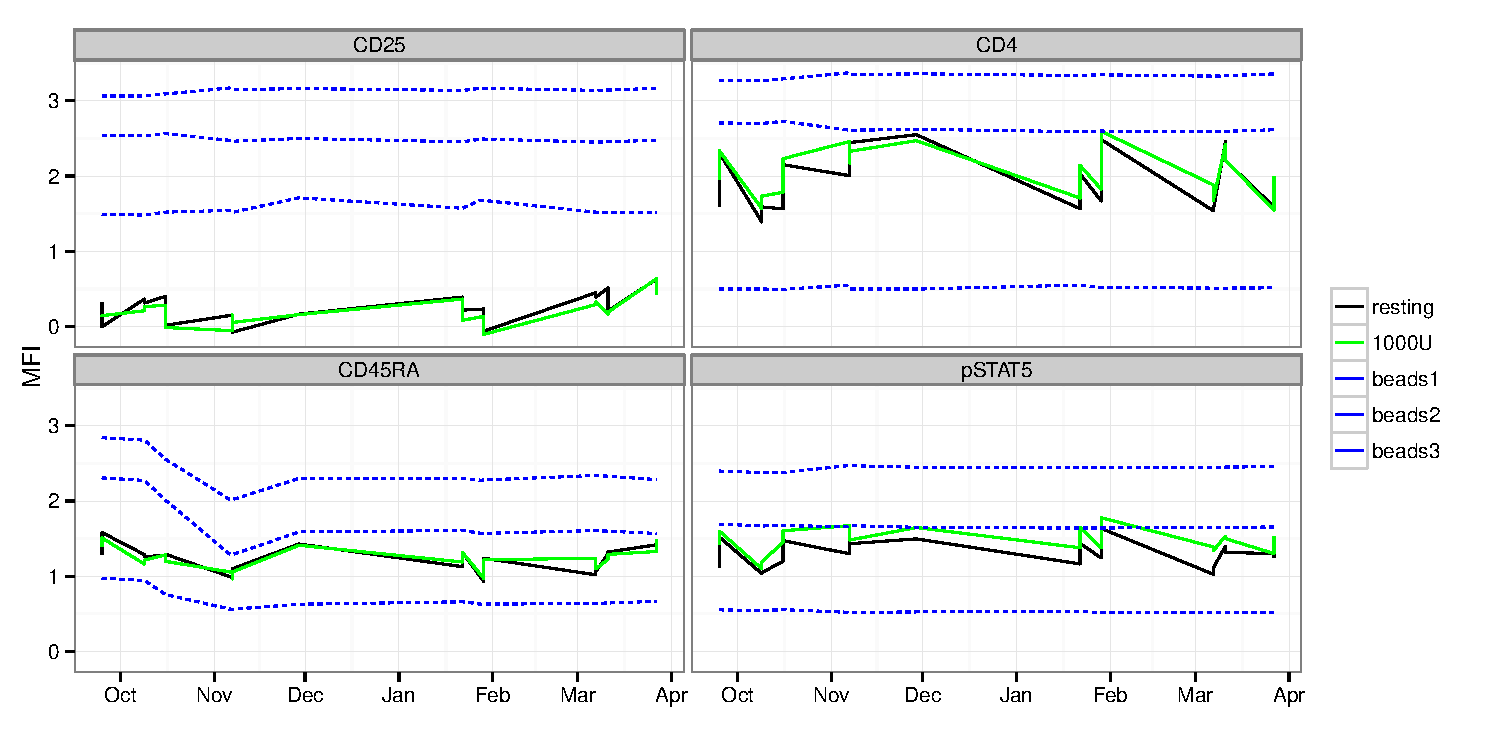
\includegraphics[scale=.5]{IL2/figures/beads.pdf}
    %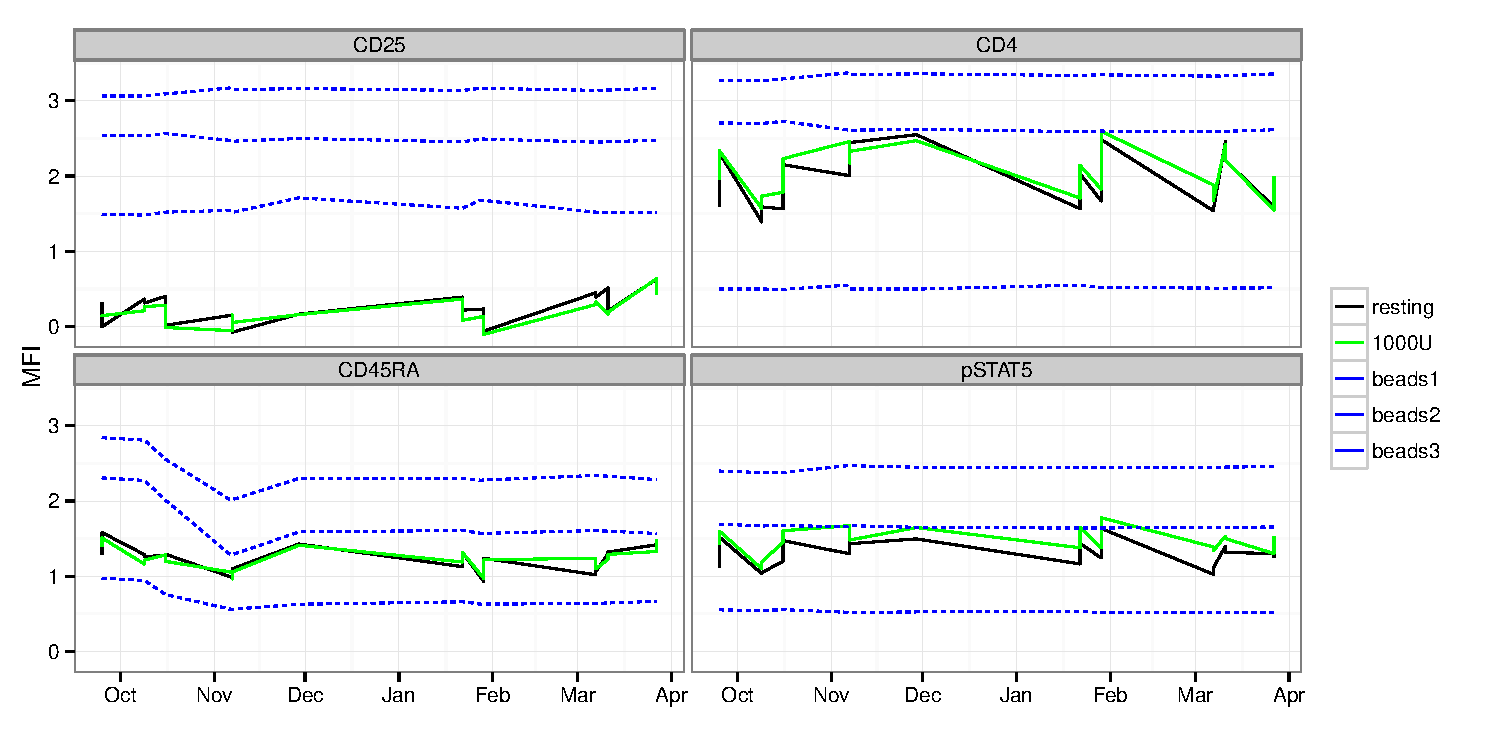
\includegraphics[scale=.5]{IL2/figures/beads.pdf}
    %\includegraphics[scale=.75]{figures/alexa488-beads.pdf}
    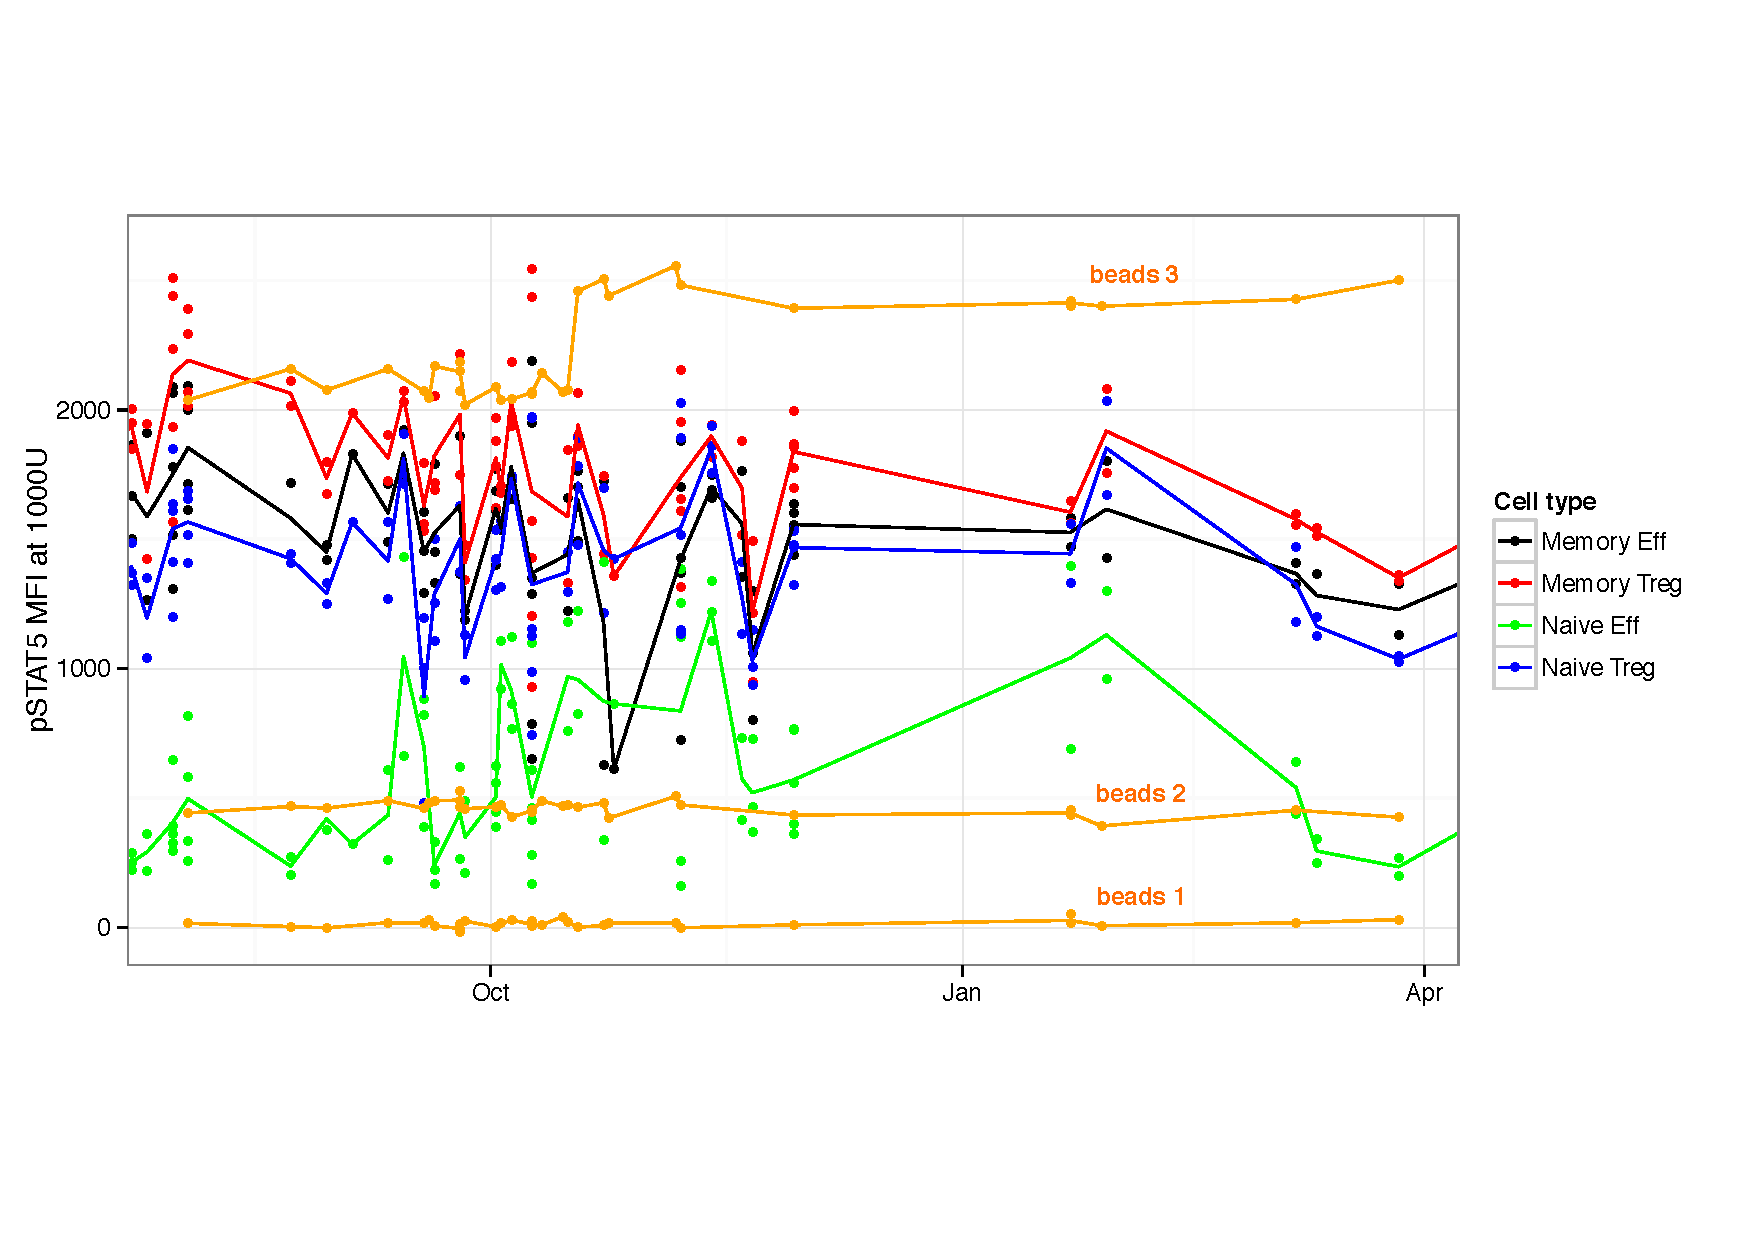
\includegraphics[scale=.6]{figures/pstat5-beads.pdf}
    \mycaption{figure:pstat5-beads}
    {Variation in sample MFI is not captured by variation in bead MFI.}
    {
      For the purpose of MFI normalisation, the fluorescence intensity of six-peak flow cytometry beads
      was measured in the Alexa 488 channel, the fluorochrome conjugated to the pSTAT5 marker.
      However, as illustrated by the loess lines, the beads are not appropriate for pSTAT5 normalisation,
      since the MFI of the three dimmest populations of beads (orange)
      does not capture the pSTAT5 MFI time variation in the four cell subsets.
      The pSTAT5 MFIs are obtained from samples stimulated at 1000 units of proleukin.
      
    }
\end{figure} 


\paragraph{ Correcting for baseline MFI }
One observation which can be drawn from \Cref{figure:dose-effect-pstat5-cellsubsets-density-repeatability} is that the
MFI of the pSTAT5 distribution in the resting sample is different across days.
If a cell population had a higher resting pSTAT5 MFI due only to day to day variability,
then one might expect that the pSTAT5 MFI in the stimulated population would also be higher.
%First I noticed that Tony had not corrected for baseline MFI.
I first attempted to account for the difference in resting pSTAT5 by subtracting the MFI of the resting population from the MFI of
the stimulated populations.
Since fluorescence intensity scales multiplicately, I also attempted to do the correction by dividing by the baseline MFI
or alternatively by subtracting the log transformed MFIs.
However, this did not appear to improve the repeatability significantly but instead just reduced the MFI by the same factor on both days
(\Cref{figure:pstat5-mfi-cellsubsets-repeatability}).
This suggests that the day to day variation in the resting sample MFI does not capture the variation in the stimulated population
.
\myfigure{scale=.75}{pstat5-mfi-cellsubsets-repeatability}
{ pSTAT5 MFI (black), background subtracted pSTAT5 MFI (red) }
{
  Correcting for the MFI in the resting sample does not appear to improve the repeatability significantly but instead just reducing the MFI by
  the same factor on both days.
  This suggests that the day to day variation in the resting sample MFI does not explain the variation in the stimulated population.
}

\clearpage

\paragraph{Nearest-neighbour joining}
%While using a different background MFI should account for differences in resting MFI,
%this assumes that the MFI difference is representative of the pSTAT5 shift.
%This may not be true for distributions which change modality.
One concern is that the difference in population cell counts across samples stimulated at different doses, may influence the accuracy of the MFI estimate.
Another concern is that since the pSTAT5 distribution is often bimodal in the cell populations considered, substracting the MFI may not be ideal.
Instead, a more correct approach would be to subtract the pSTAT5 fluorescence intensity for each resting cell.
One way of emulating this is to match each cell to its closest neighbour in the unstimulated sample.  
This was accomplished by joining samples on their core markers using the \gls{ANN} to the resting sample \citep{Jones:2011ez}
as implemented in the \Rpackage{RANN}.
This created a dataset of the same number of cells as the resting dataset, but where each cell now had a total of four functional pSTAT5 markers,
one for each stimulation dose.
At each cell it is now possible to assess the difference in pSTAT5 response between resting and stimulated states.
This is important because cells do not all have the same resting level of pSTAT5 (\Cref{figure:pstat5-baseline-relative}).
This approach presents a number of advantages.
Firstly, only the sample to which the other samples are joined needs to be gated.
Secondly, since the pSTAT5 response is relative to the baseline, it should be more robust to variation between days
and consequently, more reproducible than pSTAT5 fluorescence intensity.
Thirdly, since we have response at the cell-level, we can use methods
such as \gls{CART}, \gls{RF} and \gls{MARS} to do multivariate regression of pSTAT5 from core markers.
This could help identify cells which would have been missed from only examining core markers.
%However, even when we correct for the different baseline, the distance between the peak of the resting sample and the stimulated sample is not constant
%figure
%An advantage of this method is that number of cells per cell type is constant across doses.
%A disadvantage of this method is that the number of cells is very different of that all the cells are shifted then they will all be joined to closest neighbour
%which could be a single point.
%which will investigate in the second section.
%An alternative to this approach, would be to gate subsets in subsamples stimulated at different doses and subtract the background,
%however a clear advantage of this approach is that it allows for methods such as RF and MARS
The \gls{ANN} approach is valid without normalisation since the distributions of the core markers align across doses.
%(\Cref{figure:core-markers}).
%\Cref{figure:ann-join-0U-01U} confirms that the mapping of the clusters is correct across the nearest-neighbour mapping.
%When the between-dose variation on the core markers is negligeable,
%If we assume that the within-tube variation is negligeable, then a simpler solution is possible:
%each cell in the unstimulated subsample is joined to its closest neighbouring cell (in terms of its core markers) in a stimulated subsample.
%This assumes that the core markers are fairly stable across samples, which is usually the case in ex-vivo stimulated.
%The joining results is also not affected by any euclidean distance preserving transform, so the FCS data can be transformed before or after the \gls{ANN} joining.
%Another important check is to see whether the joining is sensitive to the transform.
%We find that we get the same results whether we join before or after the transform.
%\myfigure{scale=.3}{dose-effect-core-markers}{Dose-effect on core markers in ungated sample.} { Increasing doses represented by lines of increasing thickness.  The distributions align well across doses.  }
However, using this nearest-neighbour joining method, the repeatability of the cell phenotypes pSTAT5 MFI (\Cref{figure:nn-pstat5-mfi-cellsubsets-repeatability})
and the percent of pSTAT5\positive (\Cref{figure:pstat5-pos-cellsubsets-repeatability}) are not substantially improved.


%
%\myfigure{scale=.3}{ann-join-0U-01U}
%{ Nearest neighbour join on core markers of ungated resting sample with ungated sample stimulated at 0.1 units. }
%{
%All clusters lie on the y=x line which suggests that the largest clusters are correctly matched across samples.
%}
%
\myfigure{scale=.5}{pstat5-baseline-relative}
{ pSTAT5 intensity across the four proleukin doses, before (a) and after (b) per-cell baseline pSTAT5 subtraction in the ungated sample.}
{
  An important proportion of cells are already saturated for pSTAT5 (high baseline) in the resting sample (a).
  Correcting for the per cell pSTAT5 baseline, shows the true proportion of cells which responds to proleukin within this sample (b).
}
%
\myfigure{scale=.75}{nn-pstat5-mfi-cellsubsets-repeatability}
{ Repeatability of pSTAT5 MFI in the nearest-neighbour joined (black), nearest-neighbour background subtracted (red). }
{
  %nearest-neighbour joined samples (black)
  %nearest-neighbour joined samples baseline corrected (red)
  Background subtraction does no substantially improve the repeatability of the pSTAT5 MFI phenotype.
}
%
\myfigure{scale=.75}{pstat5-pos-cellsubsets-repeatability}
{ Repeatability of percent pSTAT5\positive in the individual samples (black), nearest-neighbour joined (red) and nearest-neighbour joined samples baseline corrected (blue). }
{
}
%\myfigure{scale=.75}{pstat5-mfi-auc-celltypes}
%{ pSTAT5 MFI for each normalisation method.  }
%{
  %The solid lines represent the median.
  %The shaded areas represent the 25th and 75th percentile.
  %The doses at which most of the variation occurs are 1000 units for naive effectors (green),
  %10 units for memory effectors (black), 0.1 units for memory (red) and naive (blue) regulatory T cells.
  %%a) The dose-response curve for each cell type in all samples.
  %%b) The medians dose-response curve across all samples for each cell type.
%}
%\myfigure{scale=.7}{pstat5-pos-auc-celltypes}
%{ Percent pSTAT5\positive for each normalisation method. }
%{
  %The solid lines represent the median.
  %The shaded areas represent the 25th and 75th percentile.
  %The doses at which most of the variation occurs are 1000 units for naive effectors (green),
  %10 units for memory effectors (black), 0.1 units for memory and naive regulatory T cells.
  %%a) The dose-response curve for each cell type in all samples.
  %%b) The medians dose-response curve across all samples for each cell type.
  %%There are many samples which stand out as outliers and a few of them have been misgated.
%}
%
%\myfigure{scale=.5}{pstat5-auc-boxplots-celltypes.pdf} { Influence of normalisation method on pSTAT5 area under curve. } { In red the normalisation using the peak alignment in CD4\positive lymphocytes, in blue the normalisation using peak alignment in lymphocytes. }
%\begin{figure}[h]
    %\centering
    %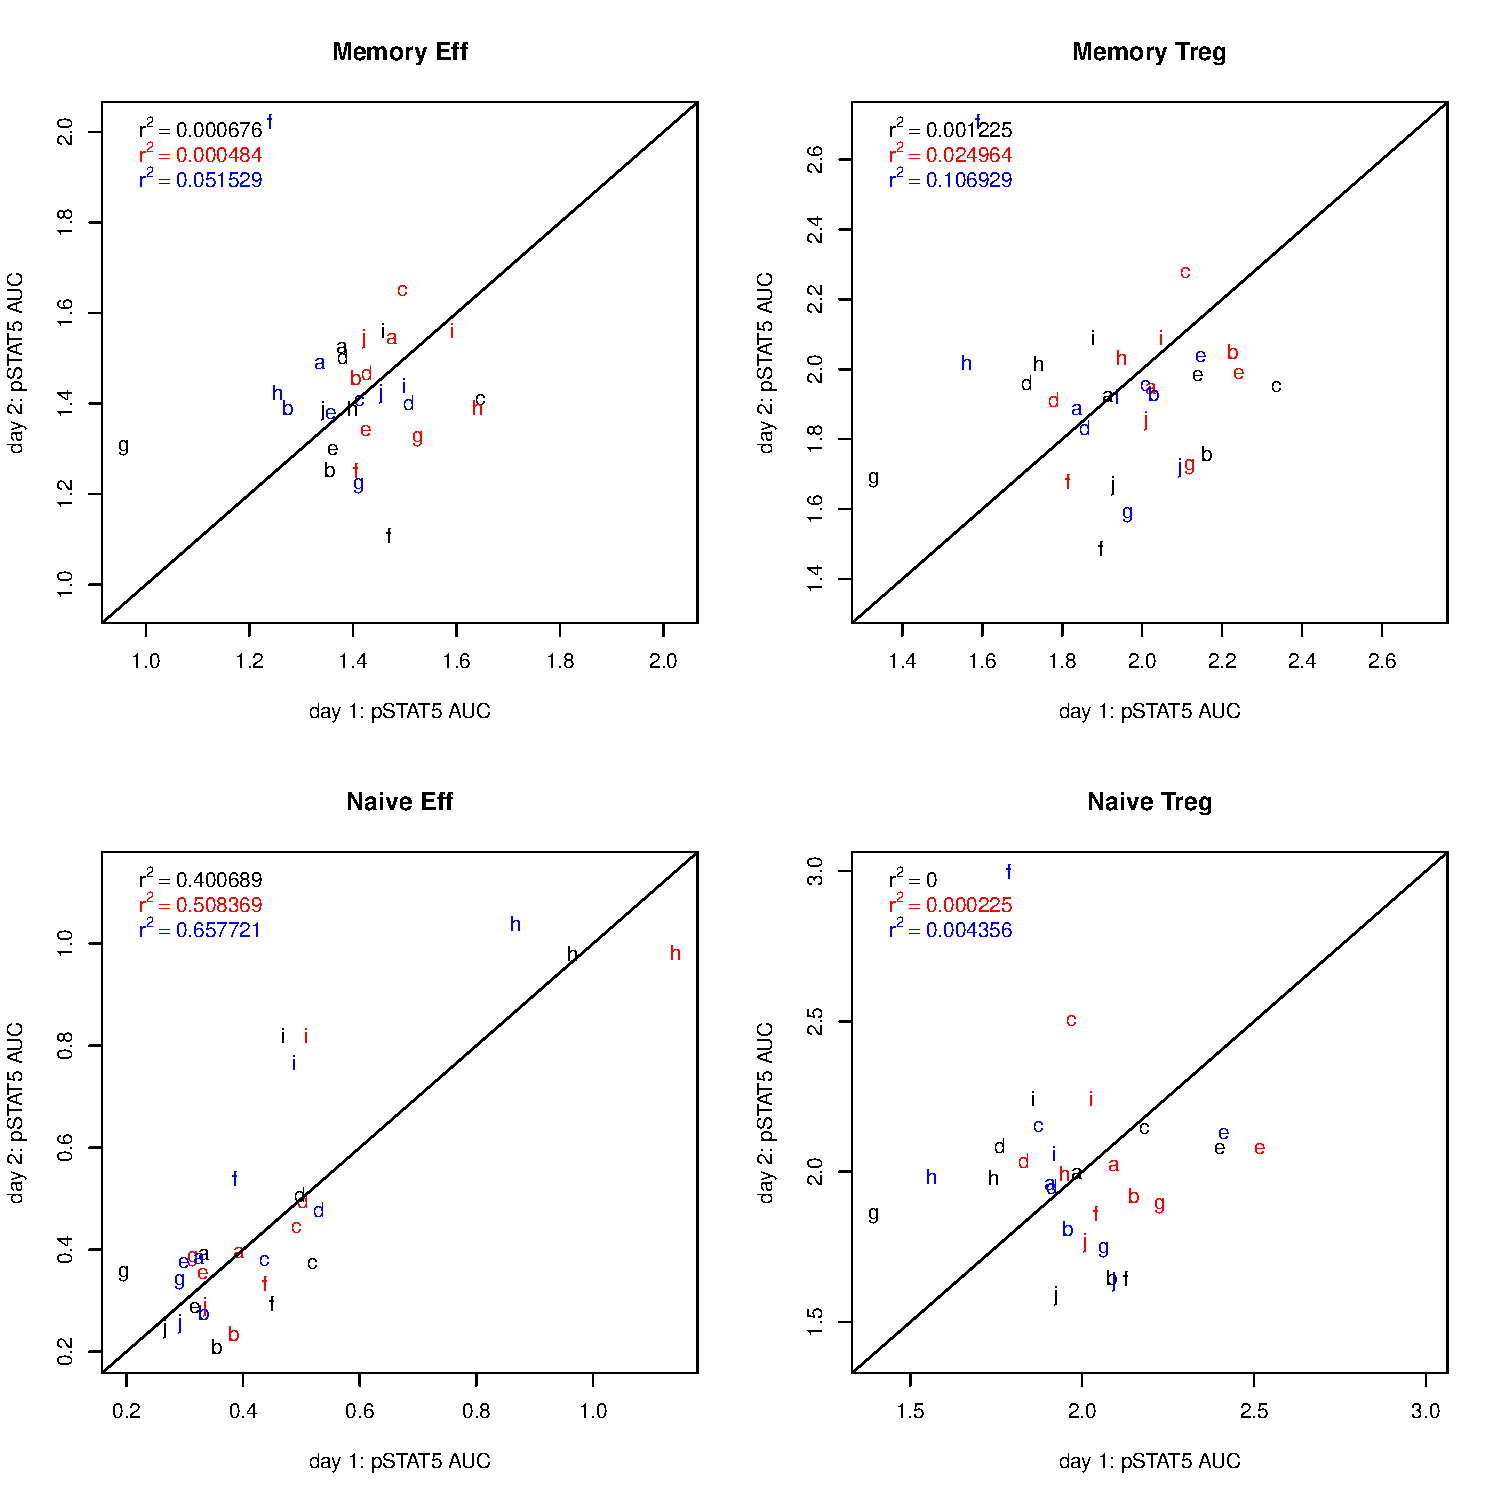
\includegraphics[scale=.5]{IL2/figures/pstat5-auc-repeatability-celltypes.pdf}
    %\mycaption{figure:pstat5-auc-repeatability-celltypes}
    %{ Influence of normalisation on the repeatability of the pSTAT5 area under the curve. }
    %{ In red the normalisation using the peak alignment in CD4\positive lymphocytes, in blue the normalisation using peak alignment in lymphocytes. }
%\end{figure}
\clearpage



\subsection{Repeatability}


For all ten repeated samples, the Pearson correlation squared $r^2$ of the MFI was assessed at the four increasing doses, in the four cell subsets,
for the raw (\Cref{figure:repeatability-PSTAT5-MFI}a),
baseline corrected (\Cref{figure:repeatability-PSTAT5-MFI}b),
nearest-neighbour joined (\Cref{figure:repeatability-PSTAT5-MFI}c)
and nearest-neighbour baseline corrected (\Cref{figure:repeatability-PSTAT5-MFI}d).
The repeatability of the percent pSTAT5\positive across doses gives a different pattern depending on the cell type
but at the highest dose it appears that the least responsive naive effector cells yield the best
repeatability (\Cref{figure:repeatability-PSTAT5-pos}).
Suprisingly, the memory regulatory T cells have the highest repeatability at the 0.1 unit dose.
The repeatability of the naive regulatory T cell phenotype is poor at all doses.  
The NN joining does not significantly improve the repeatability (\Cref{figure:nn-pstat5-mfi-cellsubsets-repeatability}).
No normalisation approach stands out as improving the repeatability.

\myfigure{scale=.5}
{repeatability-PSTAT5-MFI}
{
  Repeatability of pSTAT5 MFI measured as Pearson correlation squared ($r^2$) per dose per cell type.
}
{
  On subtracting the baseline, the repeatability of the naive effector subset is improved but not in the other cell subsets.
} 
\myfigure{scale=.5}
{repeatability-PSTAT5-pos}
{
  Repeatability of the percent of pSTAT5\positive as Pearson correlation squared ($r^2$) per dose per cell type.
}
{
  Only the pSTAT5 in the naive effector subset stimulated at 100U shows good repeatability across all normalisation methods.
  %While the repeatability of the percent pSTAT5\positive is more reproducible.
}

%
%\hspace{-2cm}
%\begin{figure}[h]
%\centering
%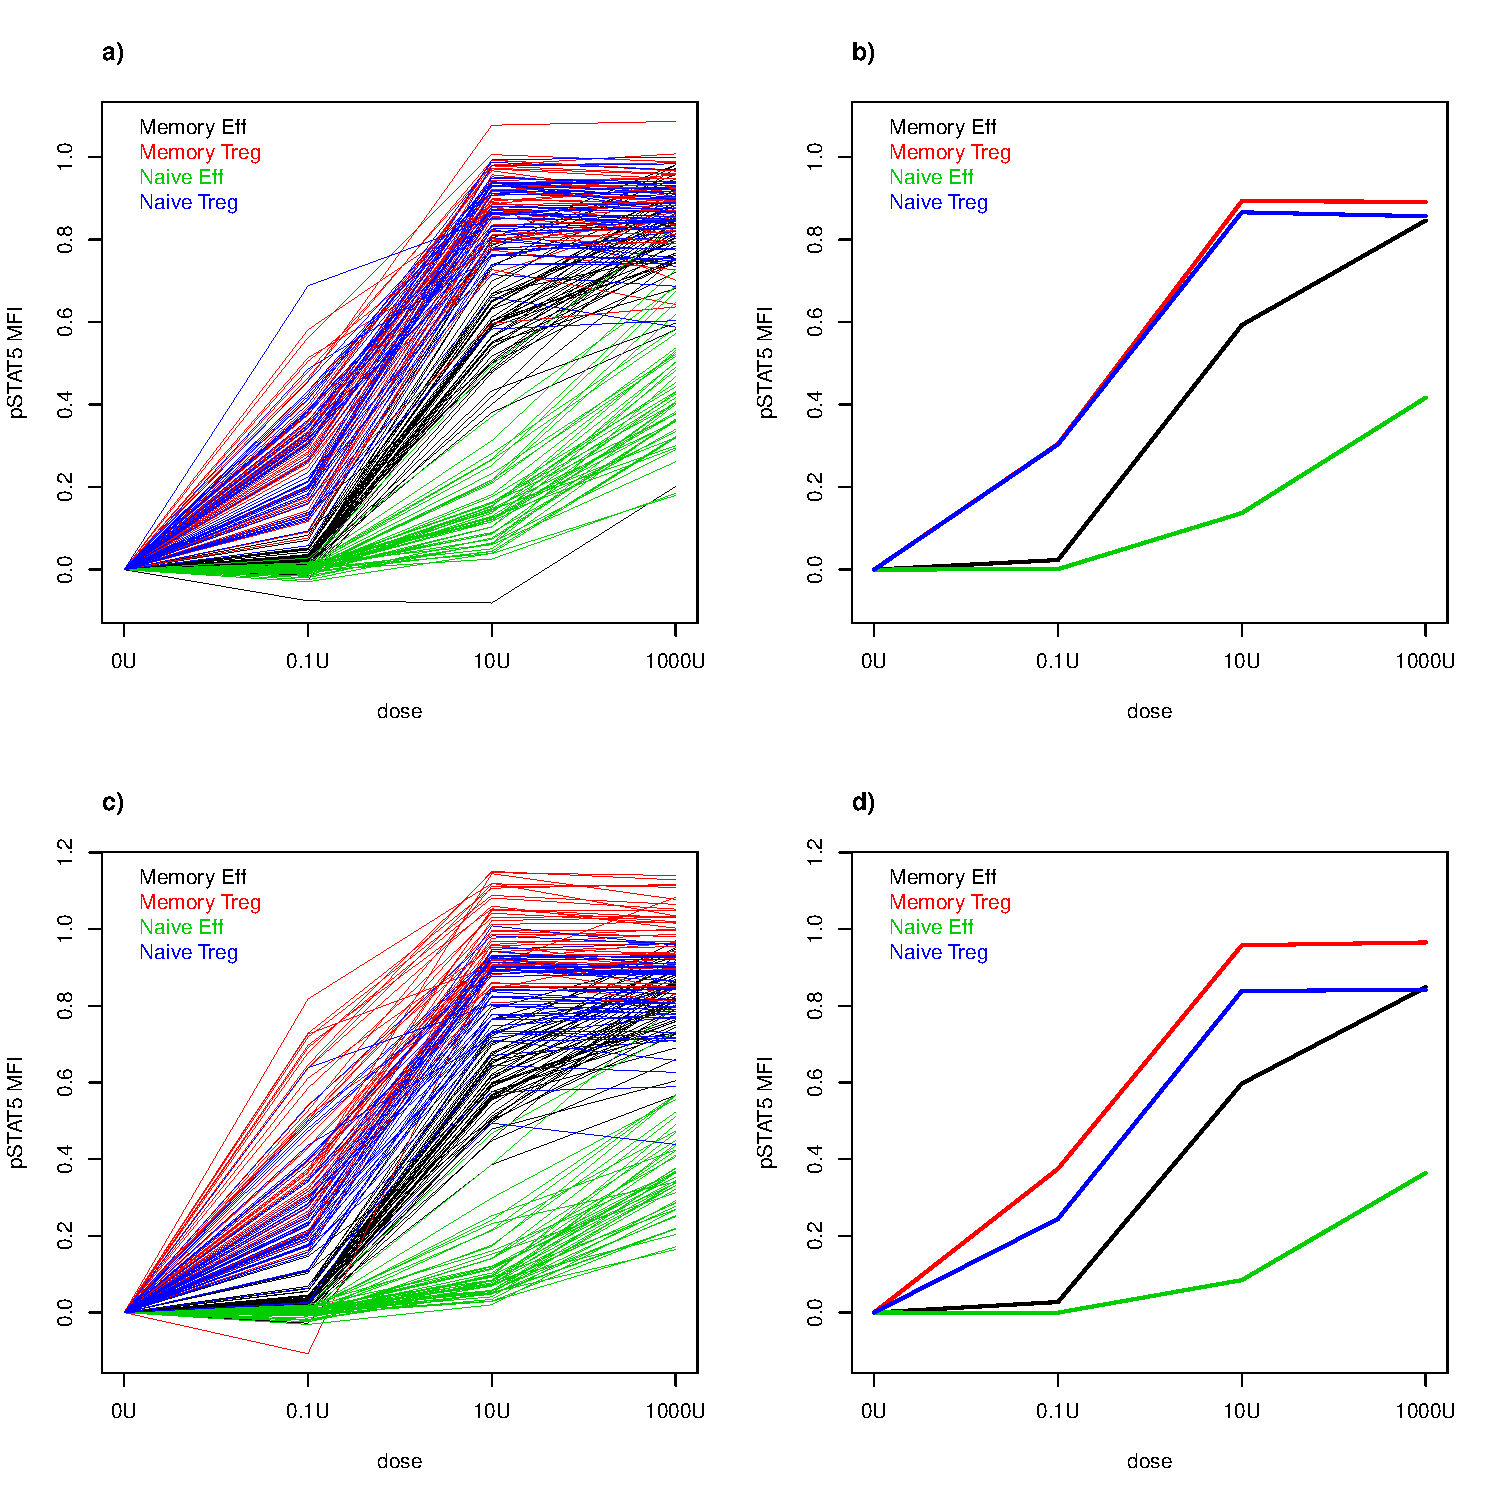
\includegraphics[scale=.4]{IL2/figures/pstat5-response-cellsubsets-manualgates.pdf}
%\caption{ \label{figure:pstat5-response-cellsubsets-gate}
%Fixed gates (a and b), magnetic gates (c and d).
%The response is measured in terms of baseline relative pSTAT5 MFI.
%a) The dose-response per cell-type in each sample obtained from manual gating with fixed gates.
%Note the outstanding memory effector sample is due to poor gating of the memory populatin in that particular sample.
%%CB01500E
%This in part due to the gate position but also because that sample does not have a clear memory population.
%b) The median dose-response per cell-type obtained from manual gating with fixed gates.
%}
%\end{figure}
%

%\section{pSTAT5 response metrics}
%\section{pSTAT5 response in the manually gated cell subsets} 
%\section{Joining samples on core markers using approximate nearest-neighbour}

%\hspace{-2cm}
%\begin{figure}[h]
%\centering
%%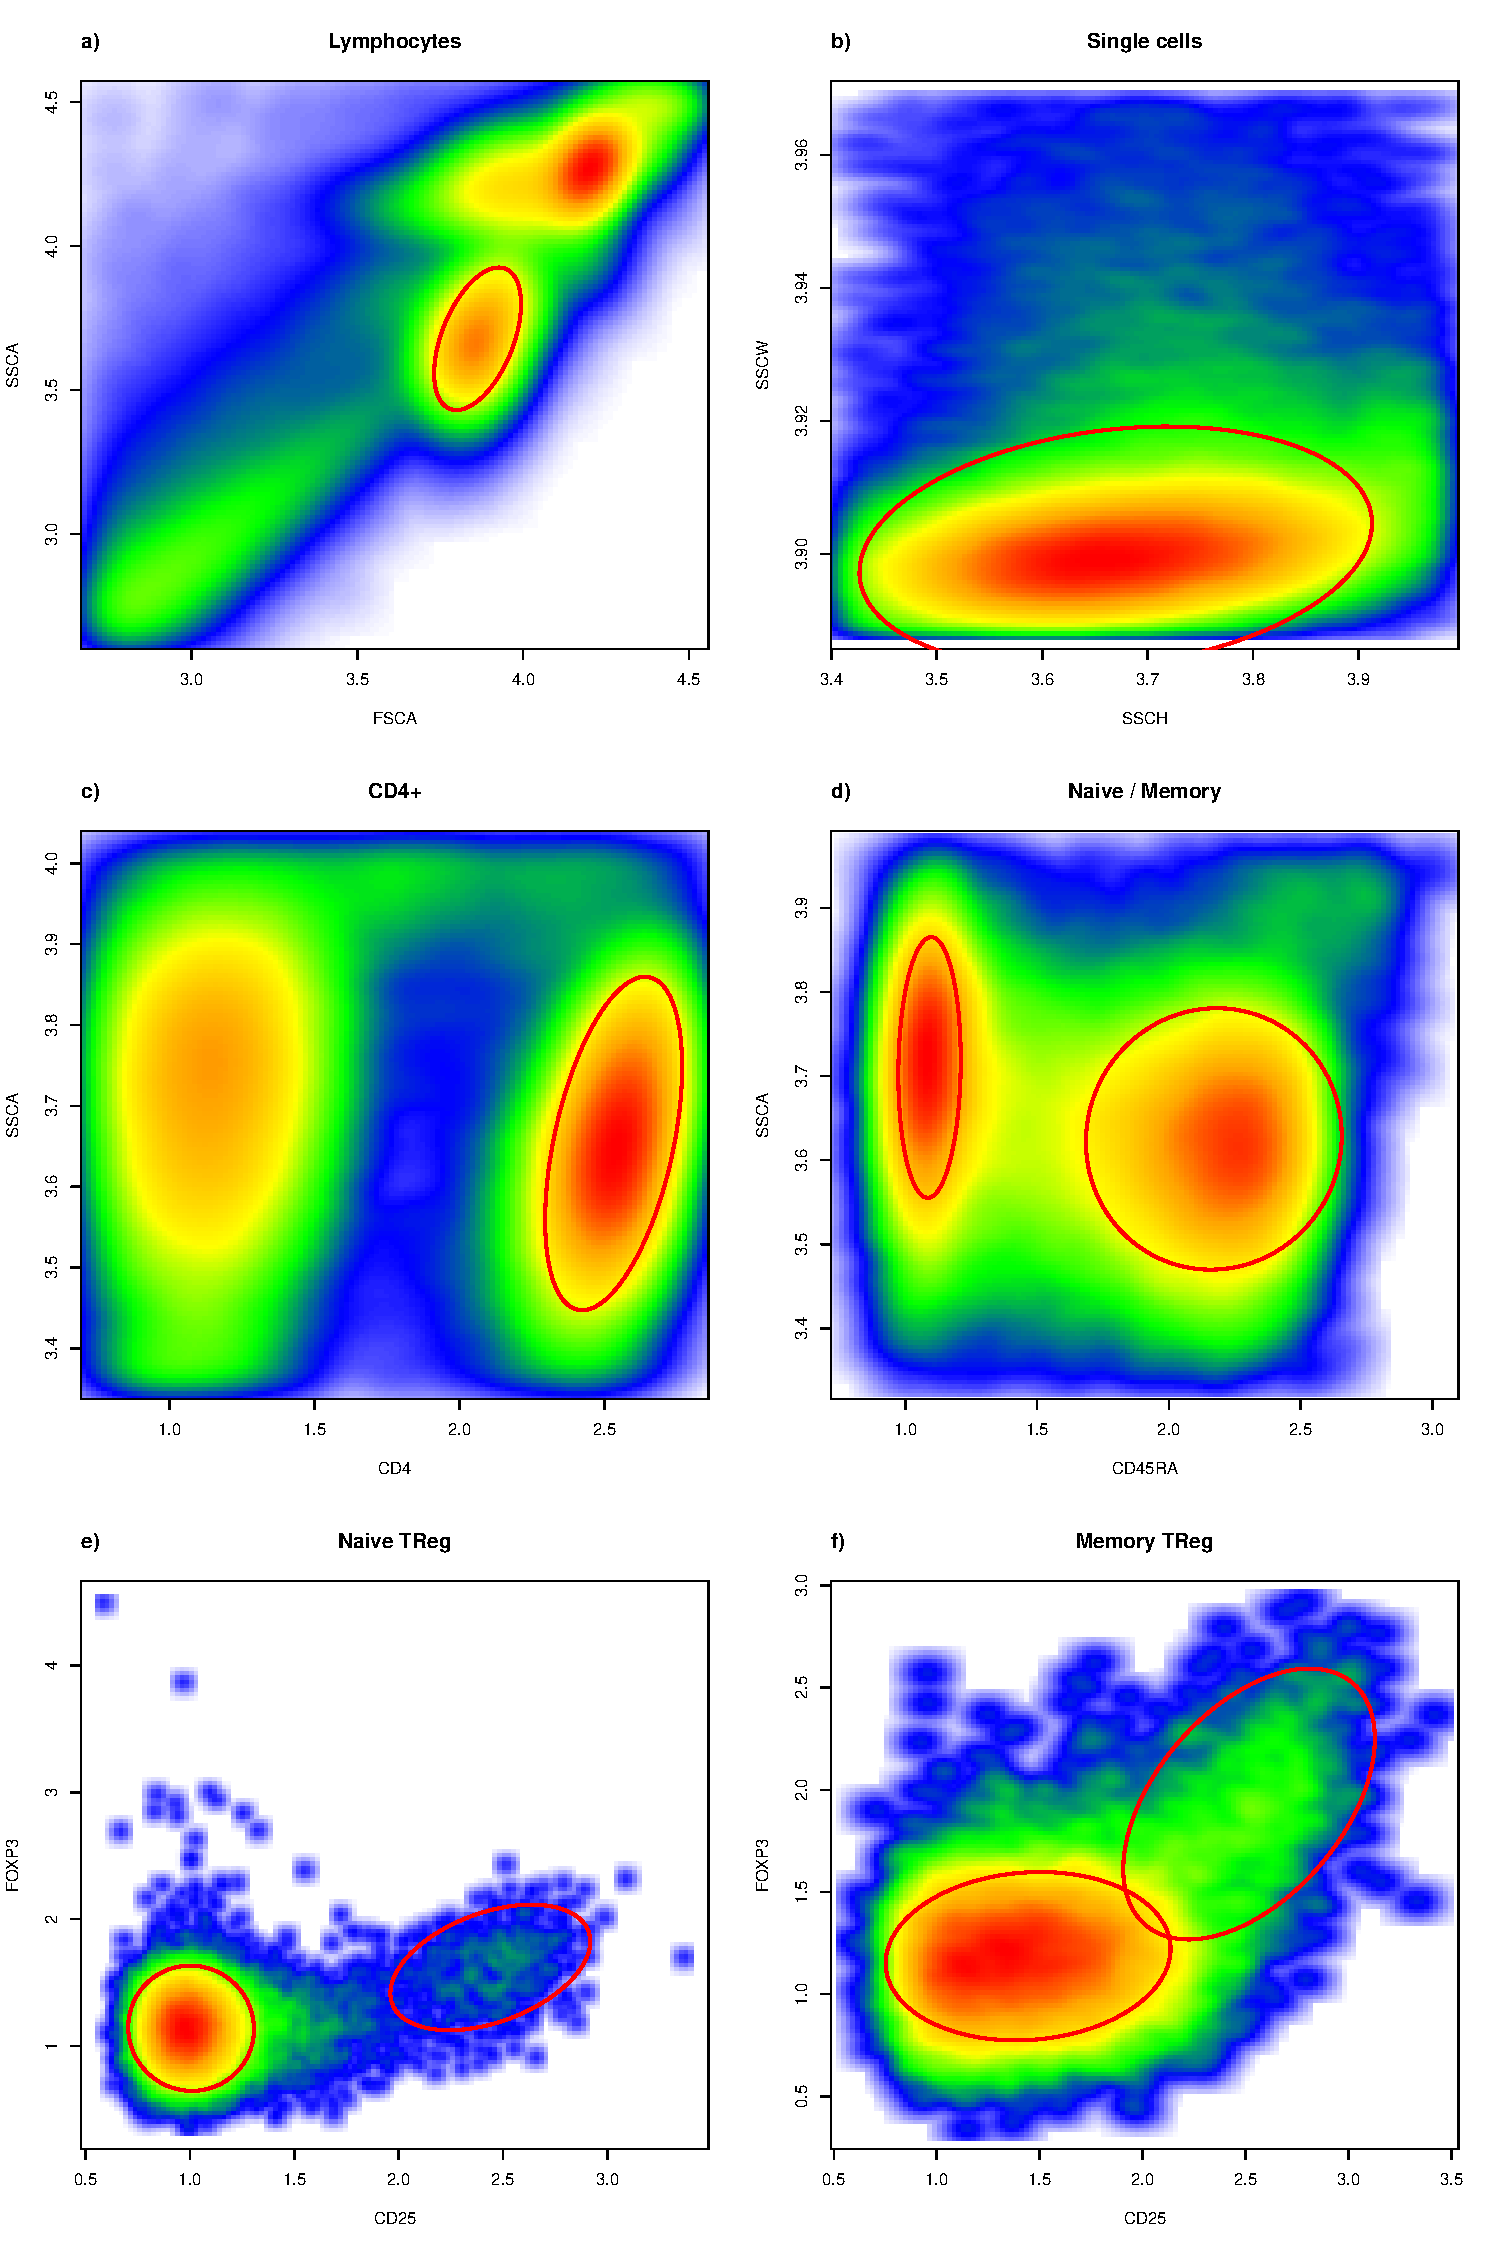
\includegraphics[scale=.5]{figures/manual-gating.pdf}
%\begin{subfigure}[b]{.4\textwidth}
  %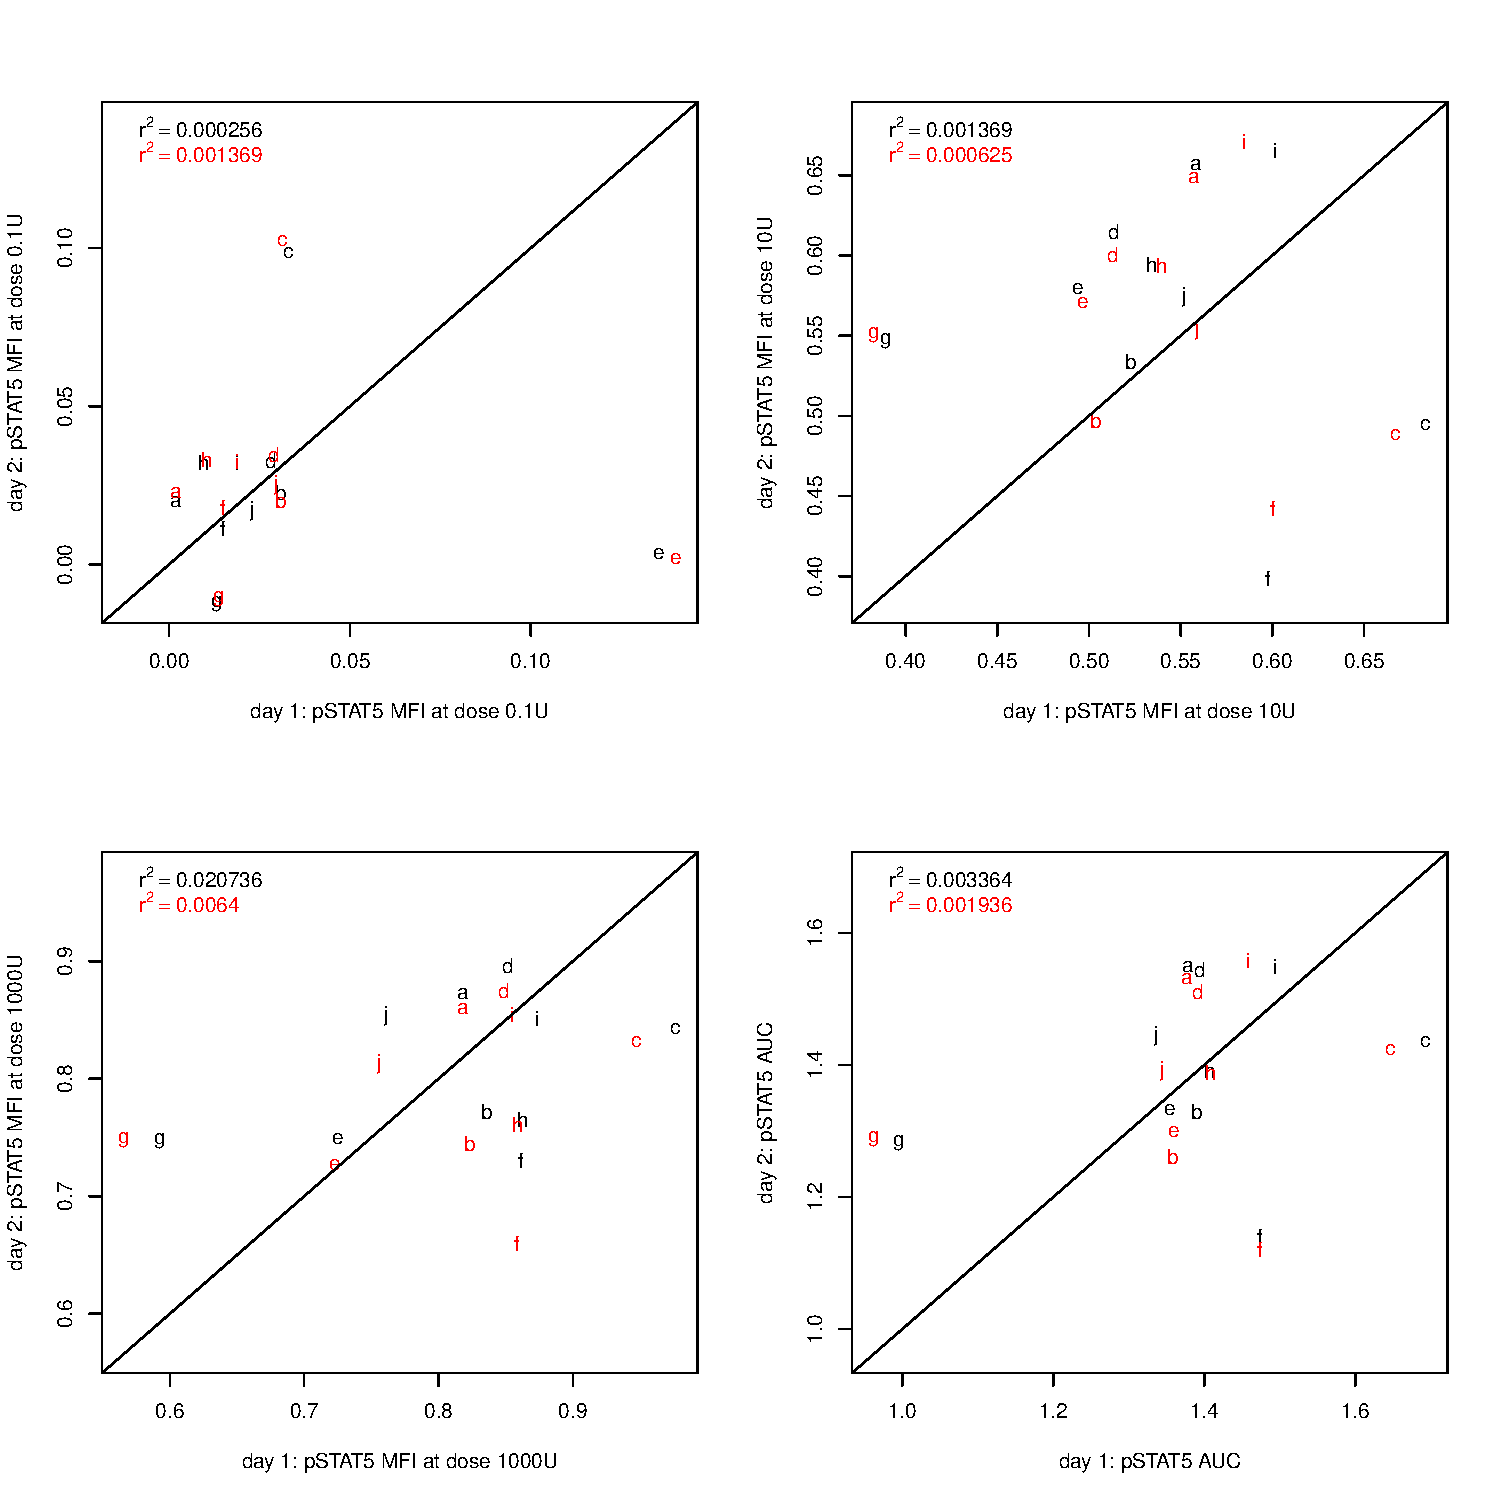
\includegraphics[scale=.25]{IL2/figures/repeatability-pstat5-mfi-Memory-Eff.pdf}
%\caption{Memory Effector}
%\end{subfigure}
%\begin{subfigure}[b]{.4\textwidth}
  %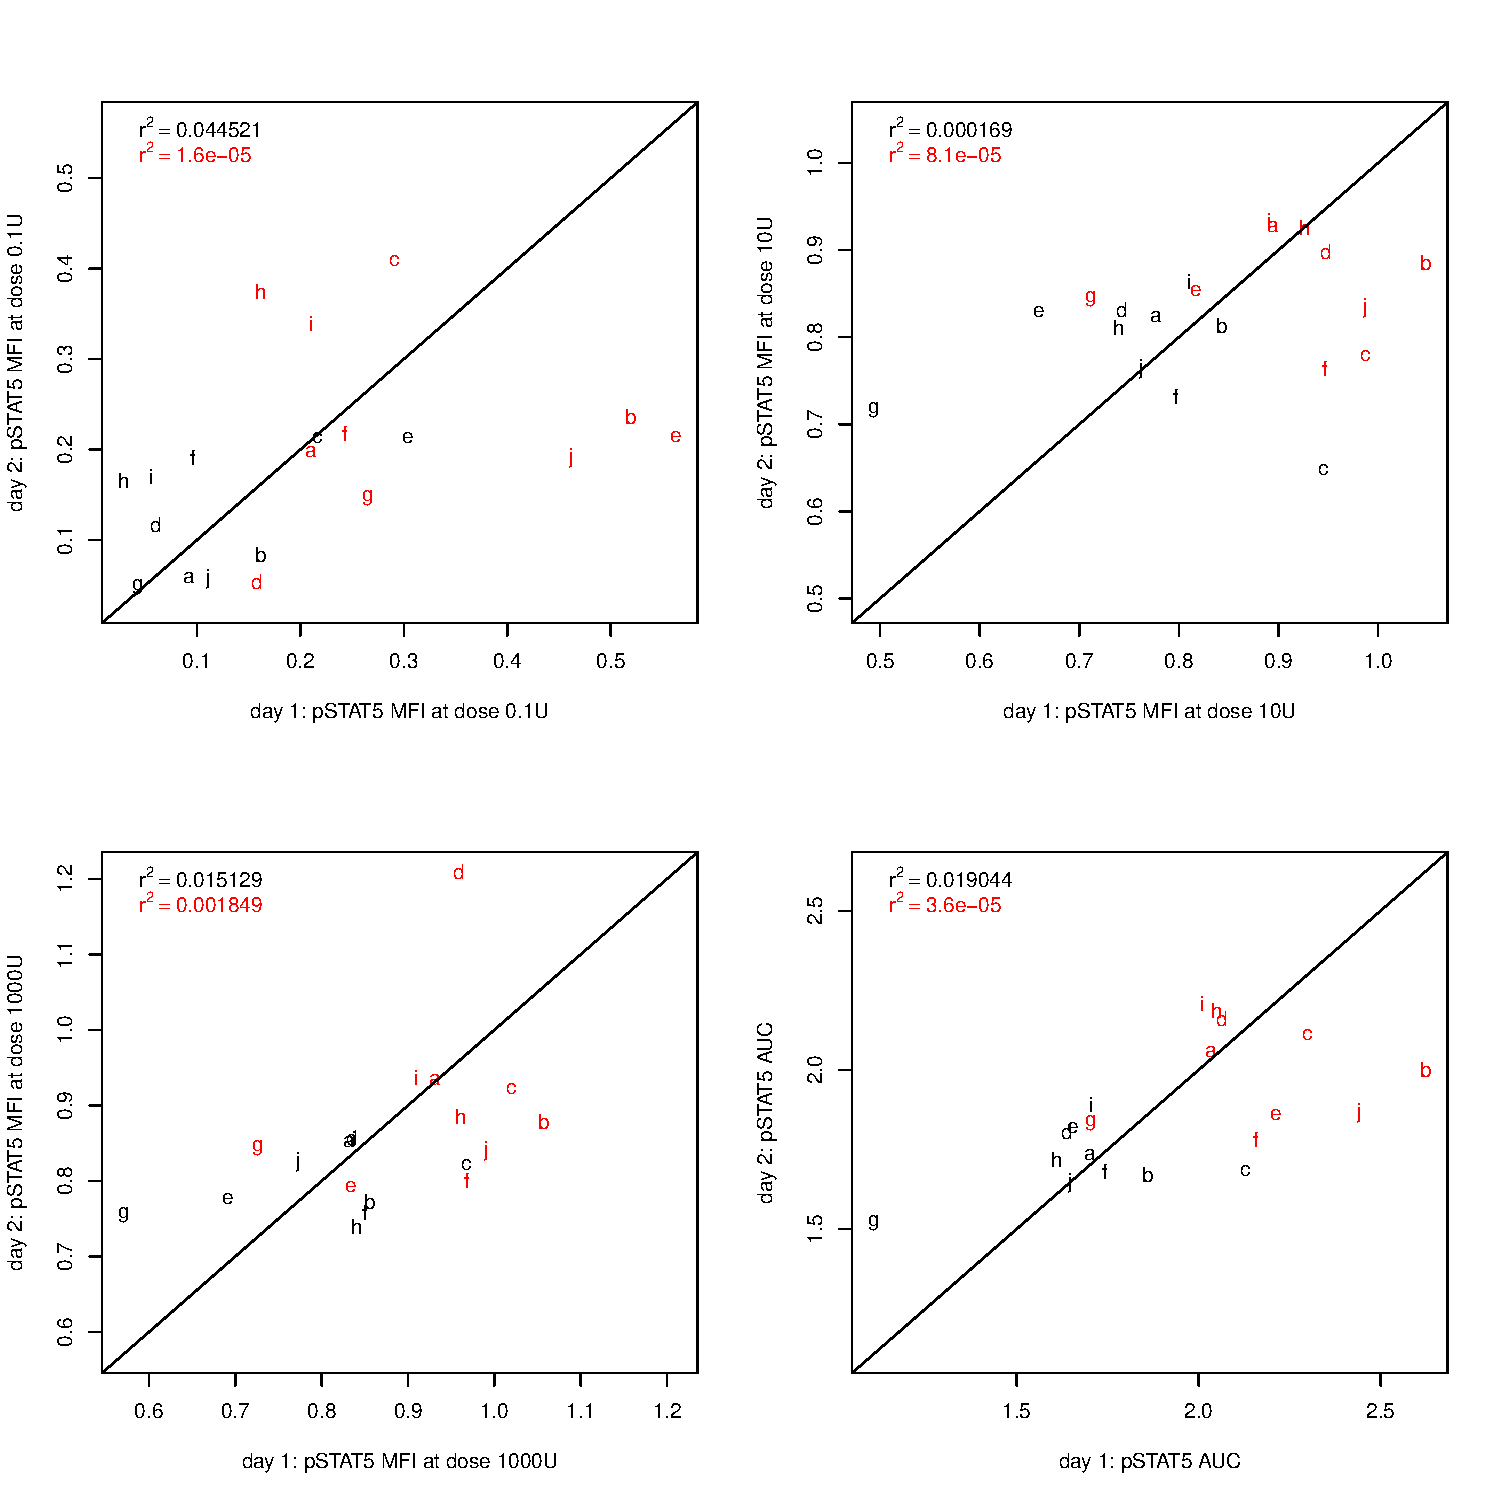
\includegraphics[scale=.25]{IL2/figures/repeatability-pstat5-mfi-Memory-Treg.pdf}
%\caption{Memory Treg}
%\end{subfigure}
%\begin{subfigure}[b]{.4\textwidth}
  %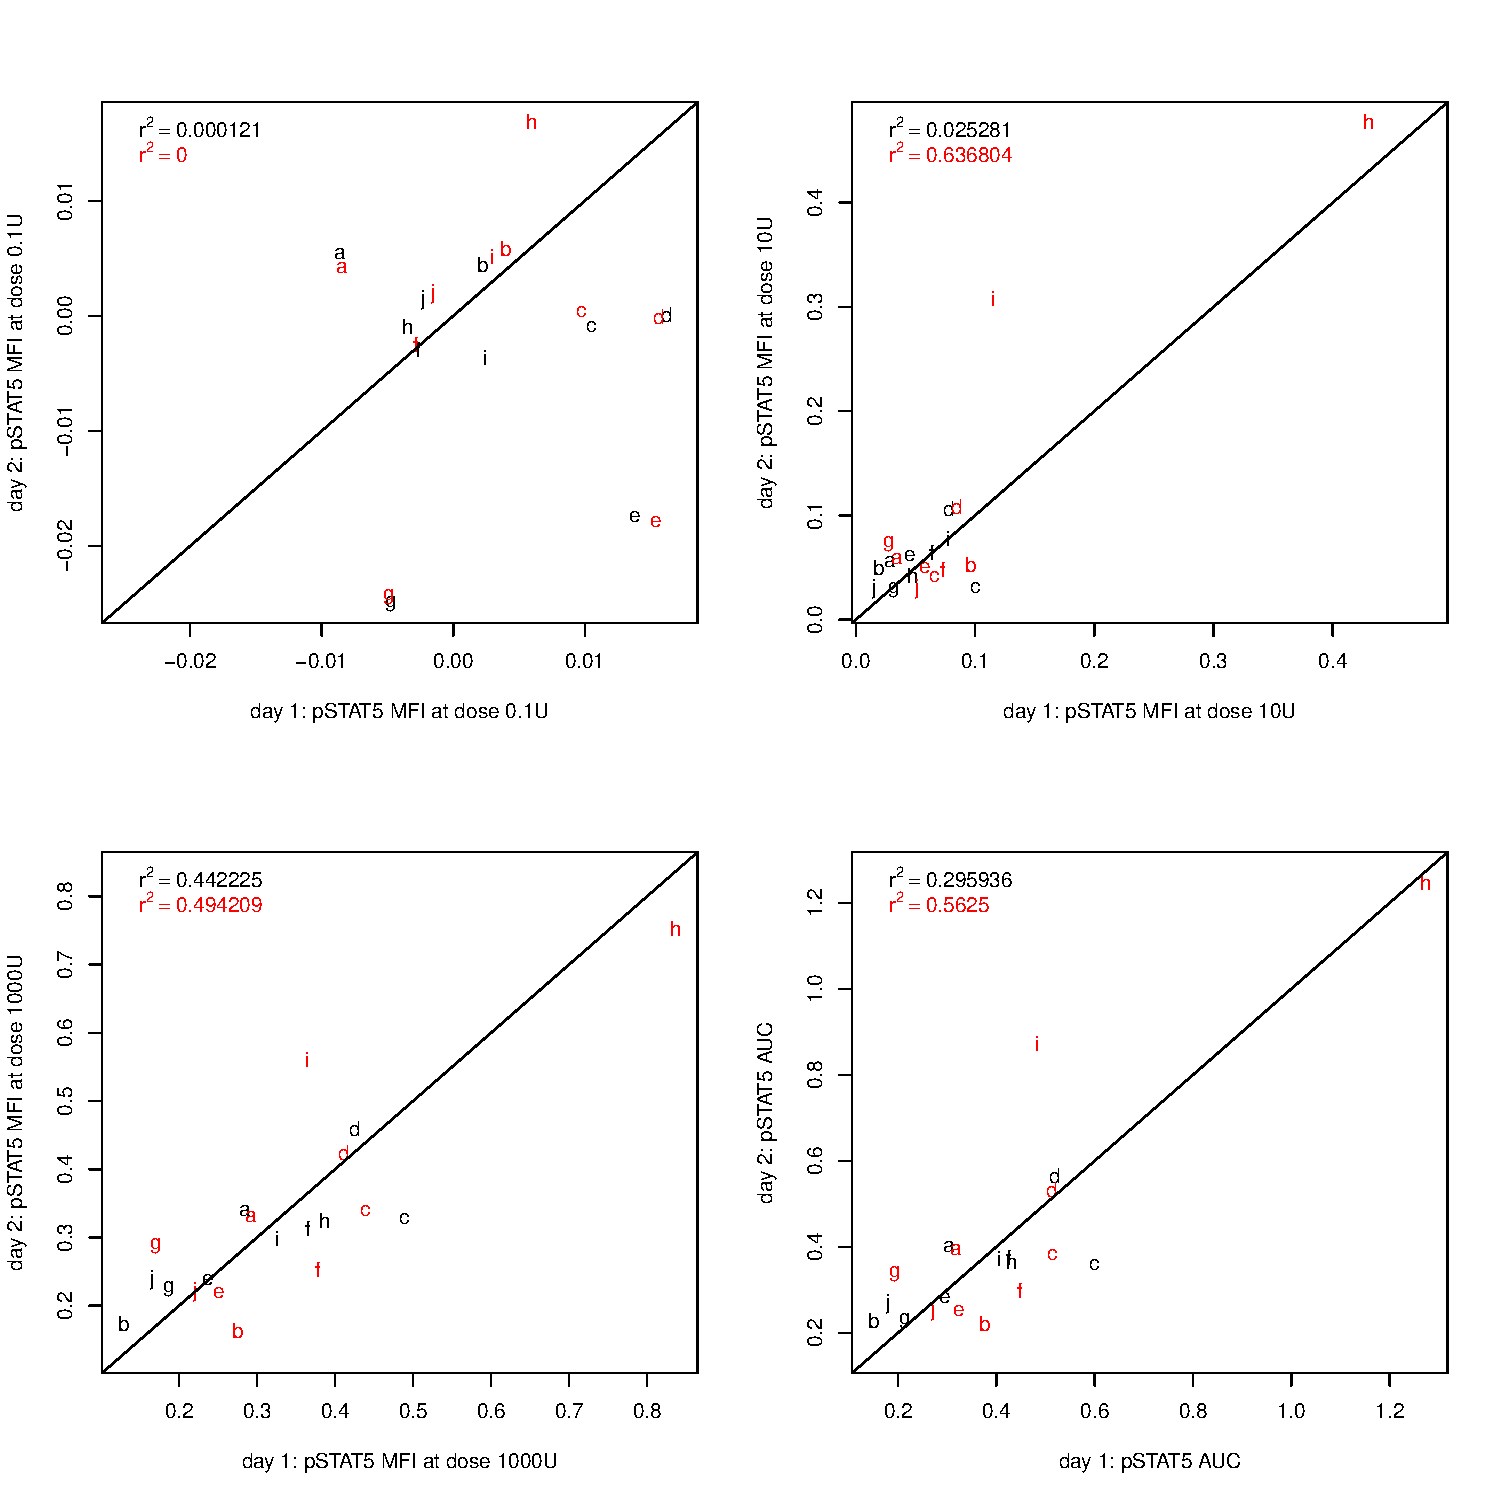
\includegraphics[scale=.25]{IL2/figures/repeatability-pstat5-mfi-Naive-Eff.pdf}
%\caption{Naive Effector}
%\end{subfigure}
%\begin{subfigure}[b]{.4\textwidth}
  %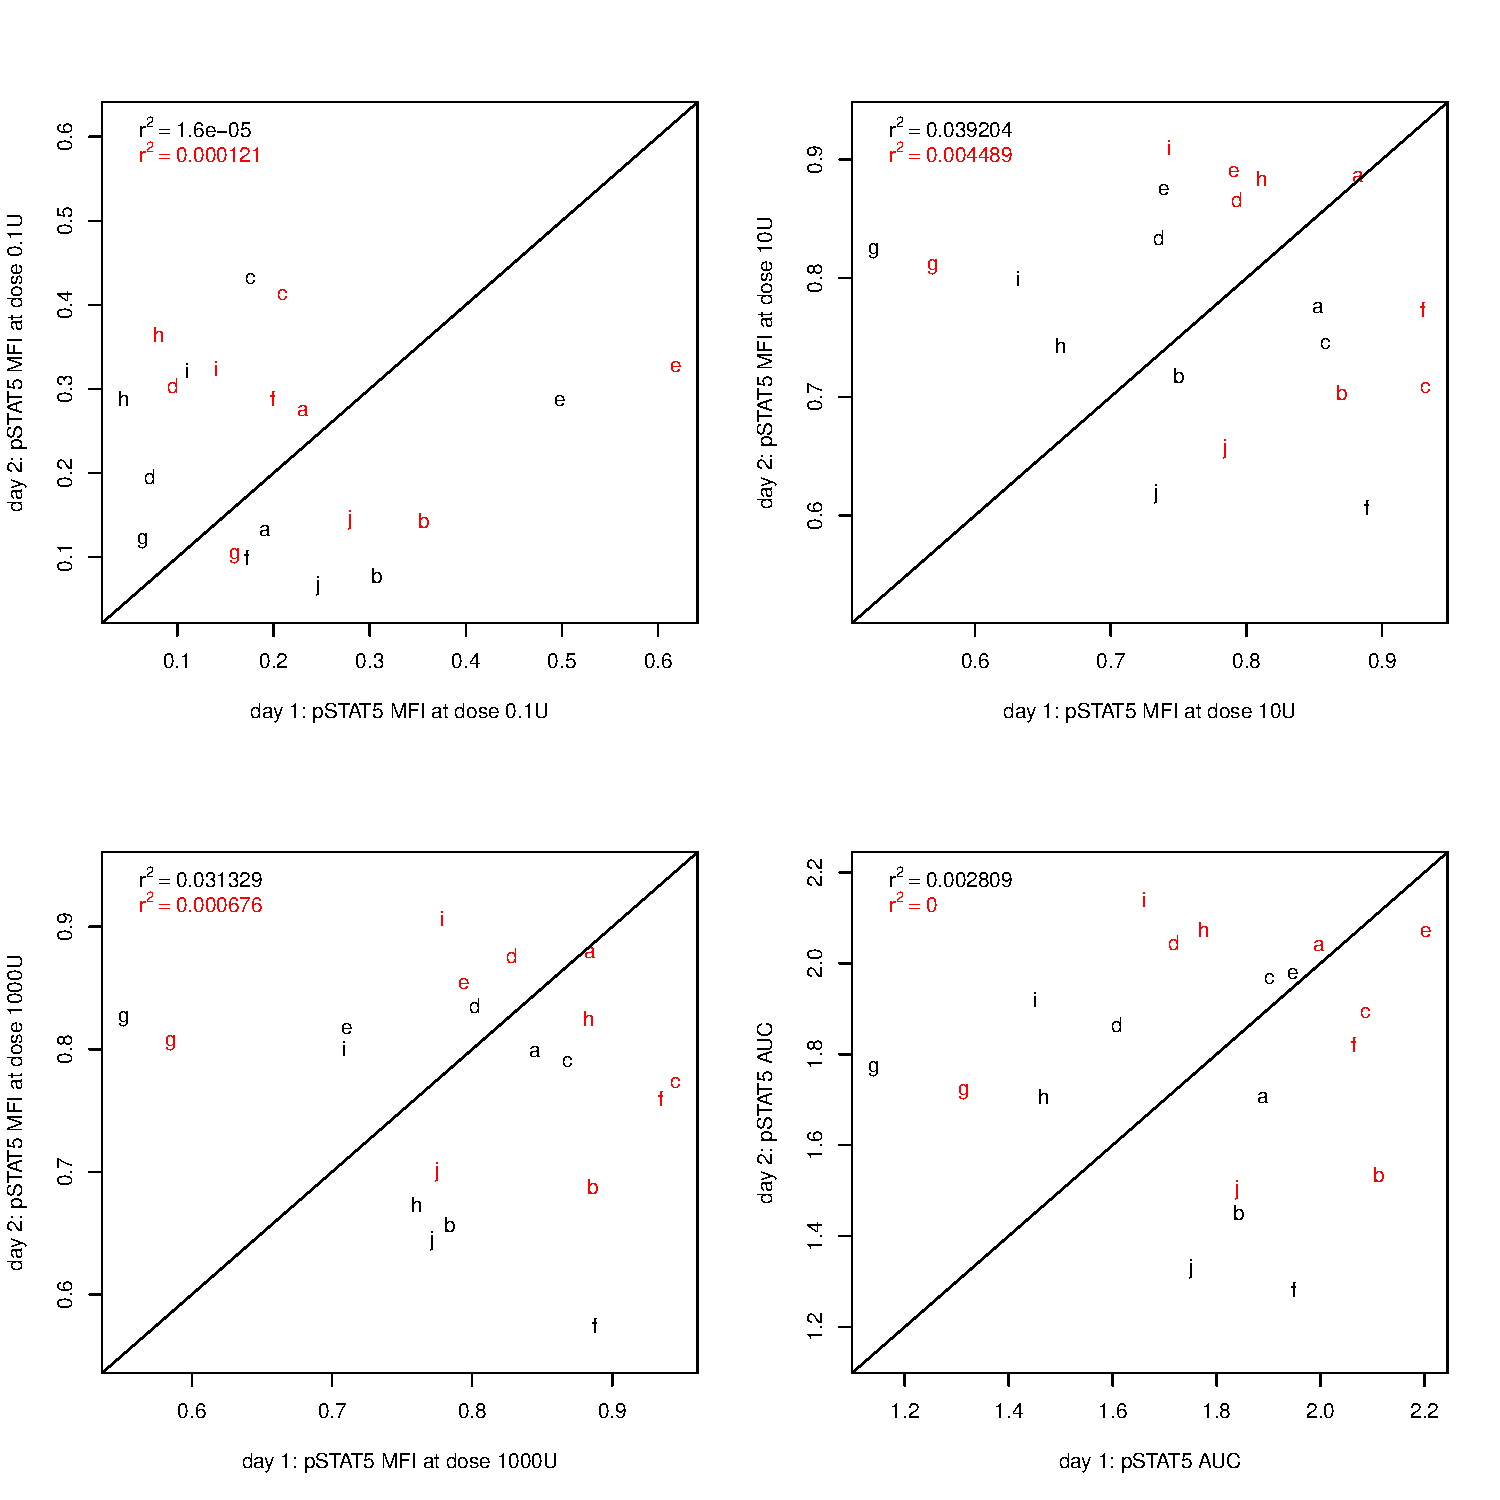
\includegraphics[scale=.25]{IL2/figures/repeatability-pstat5-mfi-Naive-Treg.pdf}
%\caption{Naive Treg}
%\end{subfigure}
%\caption{
%\label{figure:repeatability-gating}
%In black manual gates, in red magnetic gates.
%The AUC is the area under the dose response curve.
%}
%\end{figure}
%

%In the manual analysis conducted by Tony Cutler, he found that he could identify individuals which were low or high responders.
%This leads us to hypothesise that within one individual the response to \emph{IL-2} on day 1 should be comparable to the response to \emph{IL-2} on day 2.

%One method we have tried is based on the assumption is that in the ungated data, the bottom and top percentile of the pSTAT5 distribution do not respond to \emph{IL-2} and so can be used as reference points.  This is effectively a quantile normalisation method aligning the bottom and top percentile across doses.

%However we found that this normalisation method d is not true in CD4+ lymphocyte gated data.  
%Certain normalisation methods make assumptions about the shape of the data.
%The actual choice of normalisation depends on the characteristics of the data we wish to compare.
%Certain normalisation methods such as quantile normalisation are not appropriate since they assume the distributions have the shame shape.


%\begin{figure}[h]
%%
%%#simulated data
%%x0 <- mixtools::rnormmix(1000, mu=c(1,6), lambda=c(.3,.7))
%%x1 <- mixtools::rnormmix(1000, mu=.9*c(1,6)+2, lambda=c(.5,.5), sigma=c(2,2))
%%d0 <- density(x0)
%%d1 <- density(x1)
%%l0 <- extract.landmarks(x0,max.lms=2, bw=d0$bw)
%%l1 <- extract.landmarks(x1,max.lms=2, bw=d1$bw)
%%m <- lm(l0$lms ~ l1$lms)
%%x1.norm <- cbind(1,x1)%*%coefficients(m)
%%l1.norm <- extract.landmarks(x1.norm,max.lms=2)
%%#before align
%%pdf('~nikolas/GoogleDrive/PhD/Thesis/IL2/figures/simulation-peak-align-noise.pdf')
%%plot(d0,xlim=c(-3,11),main='', xlab='')
%%points(l0$lms, l0$dens, pch=20, cex=2)
%%lines(d1, lty=2)
%%points(l1$lms, l1$dens, pch=20, cex=2)
%%#after peak align
%%lines(density(x1.norm), lty=2, col='red')
%%points(l1.norm$lms, l1.norm$dens, pch=20, cex=2, col='red')
%%dev.off()
%%
    %\centering
    %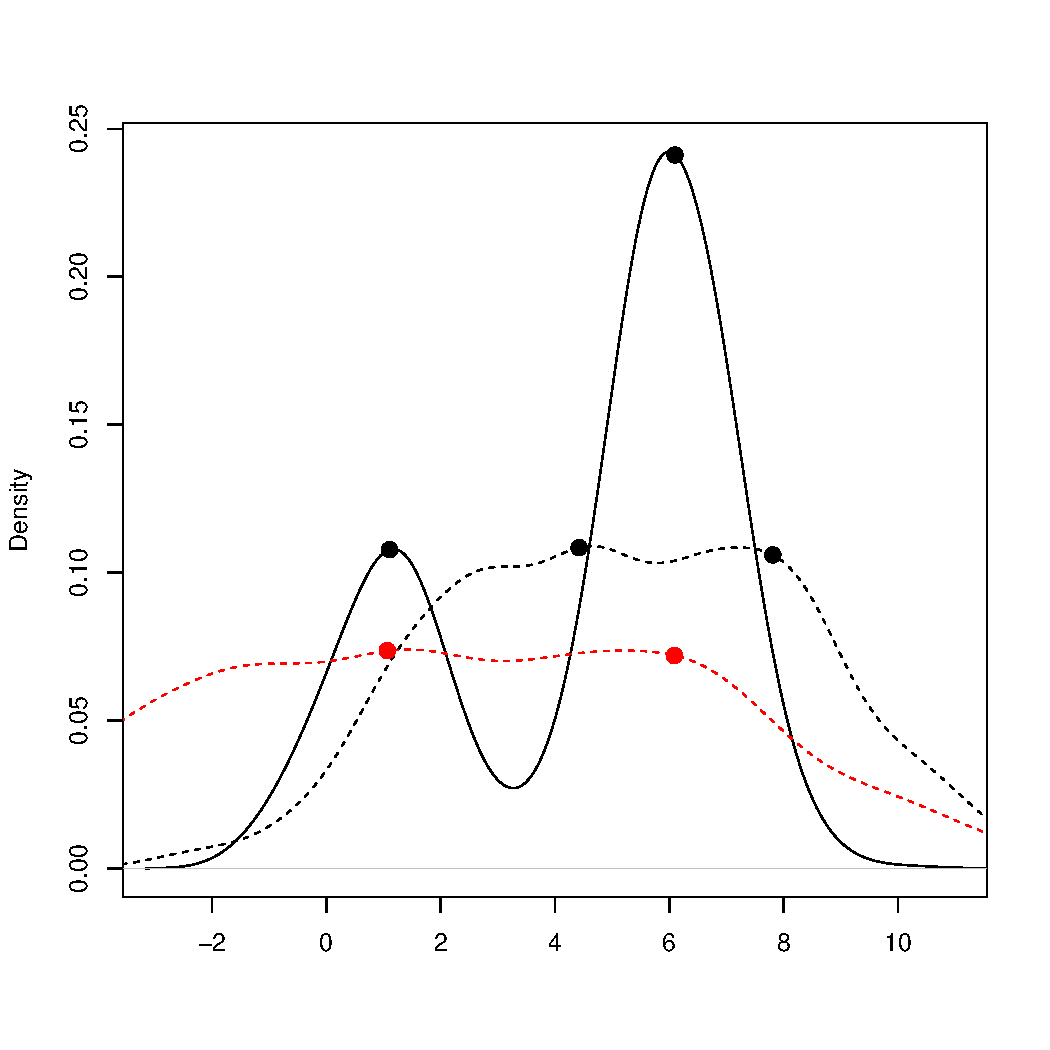
\includegraphics[scale=1]{IL2/figures/simulation-peak-align-noise.pdf}
    %\caption{  \label{figure:simulation-peak-align-noise}  In solid black line represents the density function obtained from $1000$ draws from a mixture of two normal distribution
    %with means $\mu_0=(1,6)$, standard deviations $\sigma_0=(1,1)$ and mixing proportions $\tau_0=(.3,.7)$.
    %The dashed black line represents the density function obtained from $1000$ draws from a mixture of two normal distribution
    %where $\mu_1 = 0.9 \mu_0 + 2$, standard deviations $\sigma_0=(1,1)$ and $\tau_1=(.5,.5)$.
    %The red dashed line represents the transformation using peak alignment. }
%\end{figure}
%

%%e <- lapply(flat.rep.fcs[names(flat.rep.fcs)[1:4]], function(x) ecdf(lgcl(getChannels(x, 'pstat5'))))
%%d <- lapply(flat.rep.fcs[names(flat.rep.fcs)[1:4]], function(x) density(lgcl(getChannels(x, 'pstat5')),bw=.1))
%%d.f <- lapply(d, function(d) splinefun(d$x,d$y))
%%y.max <- max(sapply(d, function(d) d$y)) 
%%e <- lapply(lymph[names(lymph)[1:4]], function(x) ecdf(lgcl(getChannels(x, 'pstat5'))))
%%d <- lapply(lymph[names(lymph)[1:4]], function(x) density(lgcl(getChannels(x, 'pstat5')),bw=.1))
%%d.f <- lapply(d, function(d) splinefun(d$x,d$y))
%%y.max <- max(sapply(d, function(d) d$y)) 
%%#pdf('~nikolas/lymph-dose-effect.pdf',width=10,height=5)
%%pdf('~nikolas/ungated-dose-effect.pdf',width=10,height=5)
%%par(mfrow=c(1,2))
%%x <- seq(-.5, 3, length.out=20000)
%%plot(x, e[[1]](x), col='white', xlab='pSTAT5', xlim=c(-.5,3), ylab='') 
%%mapply(function(e,lwd,lty) lines(x,e(x),lwd=lwd,lty=lty),e,seq(1,2.5,.5),c(1,2,2,1))
%%legend('topleft',doses, lwd=seq(1,2.5,.5), lty=c(1,2,2,1))
%%plot(x, d.f[[1]](x), col='white', xlab='pSTAT5', xlim=c(-.5,3),ylim=c(0,1),ylab='') 
%%mapply(function(d,lwd,lty) lines(x,d(x),lwd=lwd,lty=lty),d.f,seq(1,2.5,.5),c(1,2,2,1))
%%legend('topleft',doses, lwd=seq(1,2.5,.5), lty=c(1,2,2,1))
%%dev.off() 
%%pdf('~nikolas/ungated-lymph-dose-effect.pdf')
%%par(mfrow=c(1,1))
%%x <- seq(-.5, 3, length.out=20000)
%%plot(x, d.f[[1]](x), col='white', xlab='pSTAT5', xlim=c(-.5,3),ylim=c(0,1),ylab='') 
%%d <- lapply(flat.rep.fcs[names(flat.rep.fcs)[c(1,4)]], function(x) density(lgcl(getChannels(x, 'pstat5')),bw=.1))
%%d.f <- lapply(d, function(d) splinefun(d$x,d$y))
%%y.max <- max(sapply(d, function(d) d$y))
%%mapply(function(d,lwd,lty) lines(x,d(x),lwd=lwd,lty=lty),d.f,c(1,2.5),1)
%%d <- lapply(lymph[names(lymph)[c(1,4)]], function(x) density(lgcl(getChannels(x, 'pstat5')),bw=.1))
%%d.f <- lapply(d, function(d) splinefun(d$x,d$y))
%%y.max <- max(sapply(d, function(d) d$y))
%%#r <- mapply(function(a,b) length(a)/length(b), lymph[1:4], flat.rep.fcs[1:4])
%%mapply(function(d,lwd,lty) lines(x,d(x),lwd=lwd,lty=lty,col='red'),d.f,c(1,2.5),1) 
%%legend('topleft',doses[c(1,4)], lwd=c(1,2.5), lty=1)
%%dev.off()
%%lymph <- sapply(flat.rep.fcs, function(x) { cd4 <- lgcl(getChannels(x, 'cd4')); return(x[2 <  cd4 & cd4 < 2.75,]) })
%%

\subsection{Association of pSTAT5 response with type 1 diabetes}

I tested the association with T1D at each dose as well as for the area under the curve.
%Having improved the reproducibility of the cell phenotype with normalisation via peak alignment,
%we are now in a position to test the original hypothesis of whether type 1 diabetics show a reduced response to proleukin in those cell subsets.
I accounted for repeated individuals and day of analysis by including them as random effects in a linear mixed effects model as applied in \Cref{chapter:il2ra}.
%\Cref{chapter:il2ra}.
%\contributor{Hui Guo} also attempted a stratified boostrapping to compute the variance for a paired-test
%Using the paired design, we also control for sex and day of analysis.  
%Having not identified a significant association, this now brings us to the next question of whether there are other
%cell subsets besides the ones which we are gating which are sensitive to proleukin, and in particular low doses of proleukin?
%Unsuprisingly, given the small sample size and the poor reproducibility of the assay,
No T1D association was detected with the pSTAT5 MFI 
(\Cref{figure:pstat5-mfi-t1d-celltypes,figure:nn-pstat5-mfi-t1d-celltypes})
nor with the percent pSTAT5\positive
(\Cref{figure:pstat5-pos-t1d-celltypes,figure:nn-pstat5-pos-t1d-celltypes})
cell phenotypes in the four cell subsets considered.

%\begin{figure}[h]
    %\centering
    %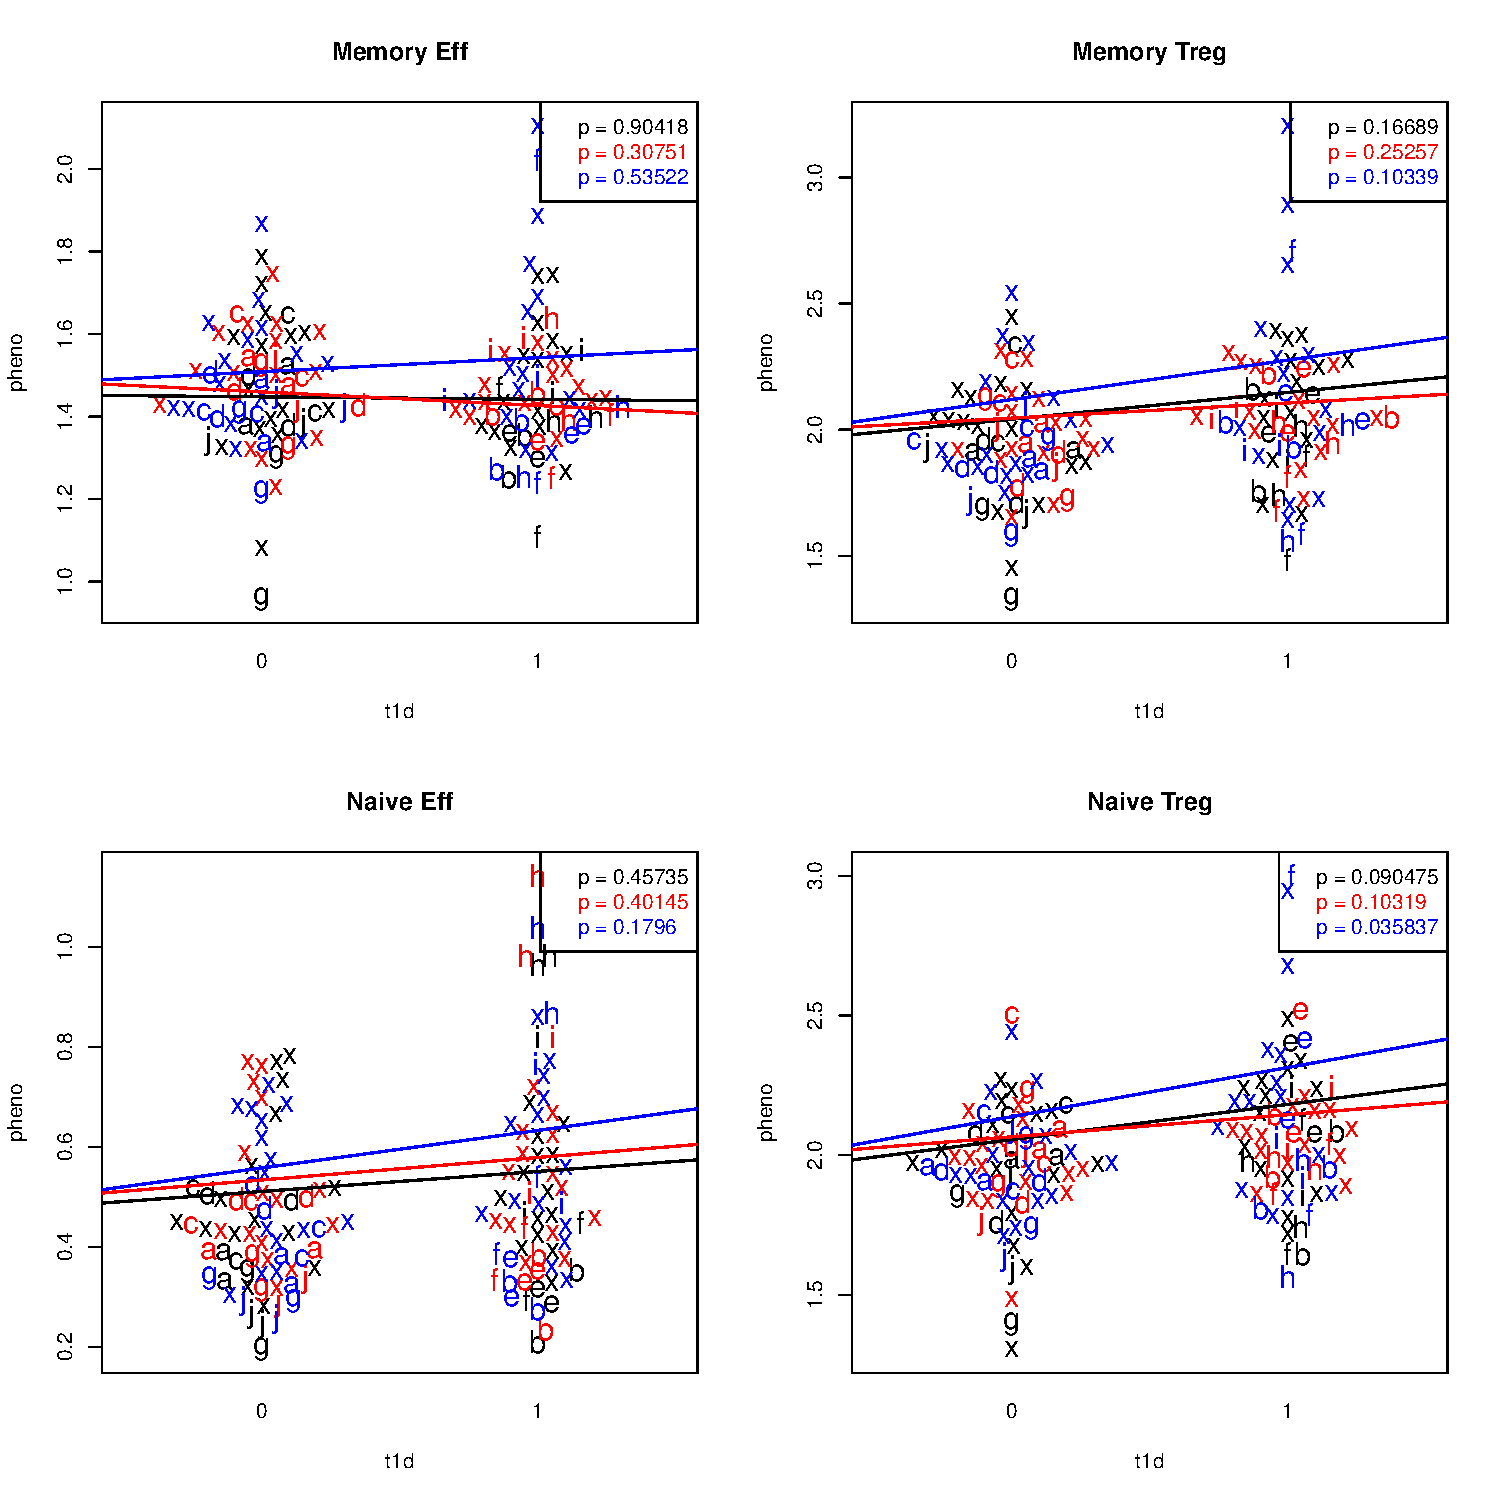
\includegraphics[scale=.5]{IL2/figures/pstat5-auc-t1d-celltypes.pdf}
    %\mycaption{figure:pstat5-auc-t1d-celltypes}
    %{ Influence of normalisation on the association of pSTAT5 area under the curve with type 1 diabetes in the four cell subsets. }
    %{ }
%\end{figure} 

% pSTAT5 MFI
%\hspace{-2cm}
\myfigure{scale=.7}{pstat5-mfi-t1d-celltypes}
{ Association test of pSTAT5 MFI with T1D. }
{ }
\myfigure{scale=.7}{nn-pstat5-mfi-t1d-celltypes}
{ Association test of pSTAT5 MFI, after nearest-neighbour normalisation, with T1D. }
{ }
{ }

% pct pSTAT5+
\myfigure{scale=.7}{pstat5-pos-t1d-celltypes}
{ Association test of percent pSTAT5\positive with T1D. }
{ }
\myfigure{scale=.7}{nn-pstat5-pos-t1d-celltypes}
{ Association test of percent pSTAT5\positive, after nearest-neighbour normalisation, with T1D. }
{ } 


\section{Response in the whole sample}

%\begin{figure}[h]
    %\centering
    %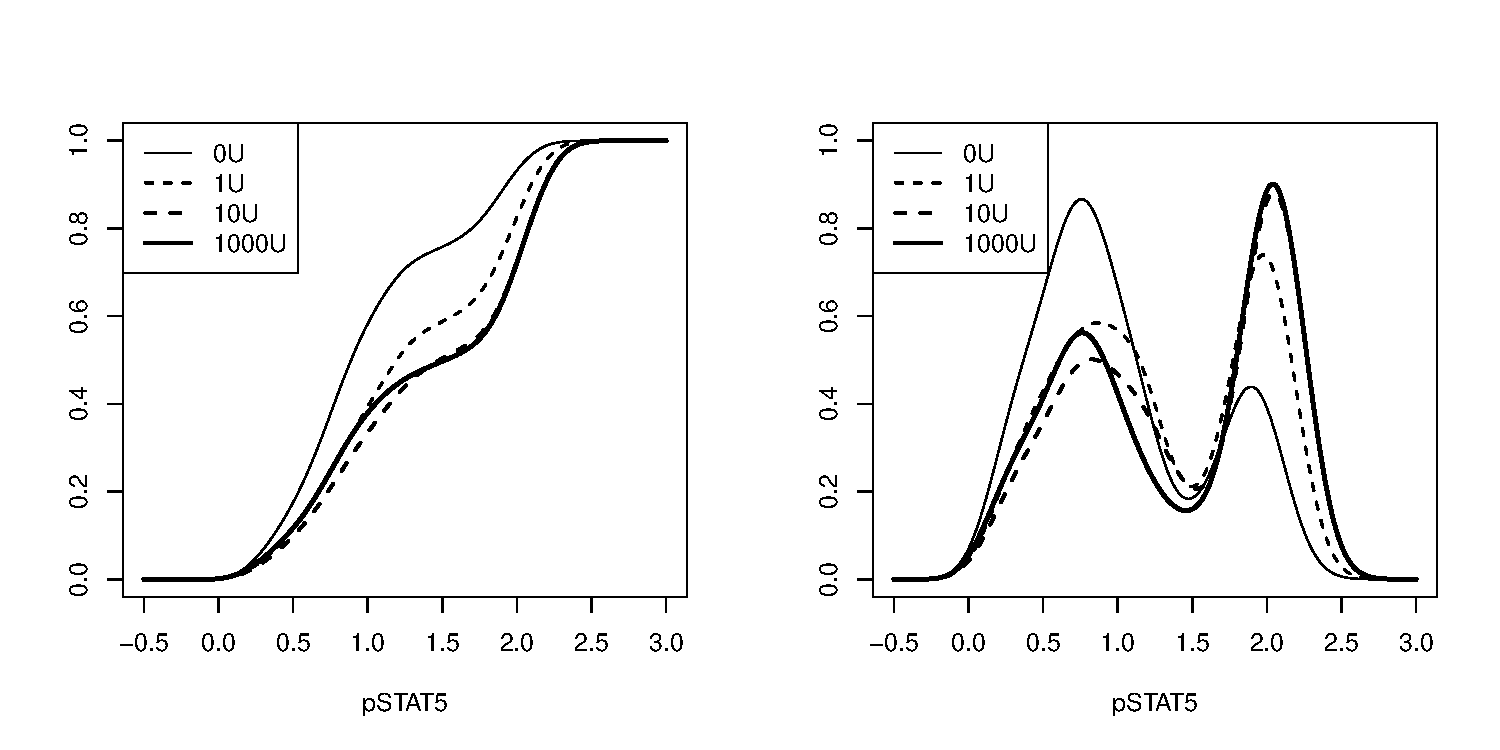
\includegraphics[scale=.5]{IL2/figures/ungated-dose-effect.pdf}
    %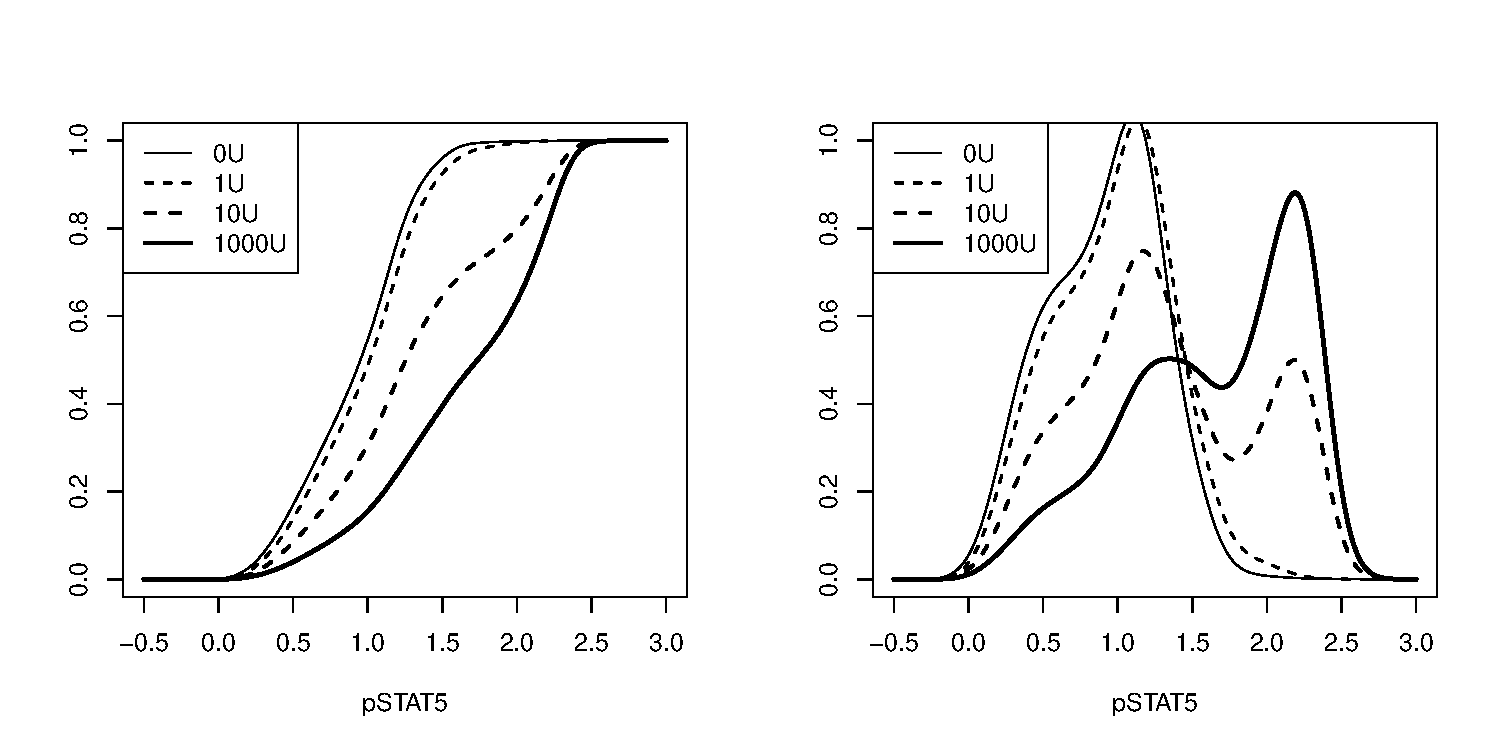
\includegraphics[scale=.5]{IL2/figures/lymph-dose-effect.pdf}
    %\mycaption{figure:dose-effect}
    %{Dose effect.}
    %{
        %On the left the cumulative density function obtained from individual a on day 1 across 4 increasing doses.
        %On the right the density function.
        %The top two figures are from the ungated sample.
        %The bottom two figures are from a CD4 range gate.
        %We observe that in the unstimulated sample the distribution is already bimodal 
        %and that upon stimulation the location of the peaks does not change much but that the height changes greatly.
        %Contrary to the ungated data, the pSTAT5 distribution in the CD4 gated sample now appears unimodal when resting or stimulated
        %at the lowest 1U dose.  At the higher doses we start seeing a bimodal distribution.
        %In the ungated sample, the location of the activation peak seems to align somewhat with that of the activation peak.  }
%\end{figure}
%
%In \Cref{figure:dose-effect} we observe that at the lowest 0.1U dose there seems to be a much more stronger relative repsonse
%in the whole sample than in the lymphocyte subset which suggests that there exist other cells beside CD4\positive lymphocytes
%which are also responsive to low doses of IL-2.  
%However the relative difference in response between 10U and 1000U seems much more important in lymphocytes than in the whole sample
%suggesting that the non-CD4\positive lymphocytes in the whole sample reach saturation at 0.1U.
%Also since the resting sample sample displays a shoulder this suggests a mixture of resting and already semi-activated lymphocytes.

DILT1D and other clinical trials of IL-2 have largely focused on lymphoyctes. %CD4\positive cells.
However, biologists know that any cell which carries high levels of any of the trimeric components of the IL-2 receptor,
alpha (CD25), beta (CD122) or gamma (CD132), should respond to IL-2, however
due to limitations on binding affinity of the CD122 antibody and the number of fluorochromes per tube,
they cannot all be included as part of every flow experiment.  
%Plus at low doses of IL-2 the CD25 chain is the most important
%Also the gamma chain is expressed by all cells and so not specific
This study of \emph{ex vivo} stimulated whole blood offers a chance to explore potentially new cell subsets responsive to IL-2.
To increase my chances of characterising unstudied cells subsets, I will be using the more complete marker panel containing CD3, CD8
and CD56 (\Cref{table:IL2-panels}) which is only available in a subset of samples.
%Given the markers used in this study, I was interested in finding out if I could identify other cell subsets which are sensitive to proleukin.
%We are interested in identifying and classifying cell subsets by their sensitivity to proleukin.  
When assessing the dose-response to stimulation in a flow cytometry sample,
the classic approach is to gate cell populations in each sample based on their core markers,
and then assess the response of the functional marker in the gated subset.
This approach may miss other dose-responsive cell populations which are not included in the gating.
%This might be solved by exhaustive gating
Here I will first explore approaches to visualise the pSTAT5 dose-response in the whole sample,
then I will consider automated gating methods which use the pSTAT5 response to guide the identification of cell subsets.
%While the manual gating inspired approach is the established method, it suffers from a major drawback:
%it relies on prior knowledge of the number of cell populations and consequently misses the pSTAT5 response in uncharacterised cell subsets.




\subsection{Visualising response in whole sample}

Reseachers working in low dimensional data typically begin with visualisation.
This is also important in high dimensional data but needs more innovative approaches.
I wanted to visualise the dose-response in the whole sample.
%\Gls{MDS} methods can give us an two-dimensional representation of a higher dimensional data set from a distance matrix.
Dimensionality reduction methods can give us a two-dimensional representation of a higher dimensional data set from a distance matrix.
%There are well established linear ones such as \gls{PCA} but also nonlinear ones such as \gls{ISOMAP} \citep{Tenenbaum:2000jp}.
These methods are particularly popular for datasets with less data points but more dimensions than flow cytometry,
as generated by mass cytometry technologies such as CytoF.
In mass cytometry datasets, more emphasis is given on uncovering cell lineages and progressions rather than discrete cell populations.
Most of these methods require computation of the complete pairwise distance matrix,
but some like \gls{PCA} use the covariance matrix instead to apply a linear transform.
%Stochastic neighbour embedding attempts to preserve the proximity of objects in higher dimensional space by using probabilistic mapping of higher dimension space to lower dimension.  A drawback is that the mapping is impossible to retrieve, which is why component methods like PCA and ICA are more interpretable.  
However, information is lost when considering only the first two components of a linear projection.
Therefore, there is considerable interest in developing methods which capture both the local and global structure of the data,
so that points which lie close in higher-dimensional space lie close in two-dimensional space.
%\gls{ISOMAP} \citep{Tenenbaum:2000jp}.
%SPADE is a methods which was developed with this objective.
\acrfull{SPADE} for example represents the data as a \acrfull{MST}, the shortest path that connects all points in a network \citep{Simonds:2011jh}.
%The visualisation requires downsampling requires downsampling.
%A soft approach to downsampling, is to downweight points in high-density regions
SPADE proceeds by first calculating the density at each data point in each of the FCS file.
The number of points is then reduced by preferentially removing 
points with high local density while preserving lower density ones,
with the objective of making the density more uniform across the sample,
so that it has less influence on the clustering.
Once the number of points has been suffciently reduced in each FCS file, the samples are pooled and hierarchical clustering is applied
on the reduced dataset.
The overall number of clusters can then be selected by cutting the resulting dendogram at the required height.
The default parameter is 300 clusters.
These clusters are then joined using the \acrfull{MST} algorithm for the purpose of visualisation.
Once the MST has been defined, the points which were discarded in the first step are added back and assigned to their closest cluster.
The same spanning-tree is then drawn for each FCS file with the size of the nodes representing the number of data points assigned to each node
in each file.
The tree nodes are coloured according to the functional marker, here pSTAT5, which was not used in its construction.  

I first ran \gls{SPADE} on the core surface markers, CD25, CD3, CD4, CD45RA, CD56, CD8 and FOXP3,
on the manually gated lymphocyte subset (excluding doublets).
The resting and stimulated at 0.1, 10 and 1000 units of proleukin,
tubes from an individual were downsampled and pooled for the clustering.
The desired number of cluster was set to 500.

in order to investigate how the manual gates map to the \gls{MST} representation.
\Cref{figure:spade-output}

\Cref{figure:spade-celltypes}

However, the generated \gls{MST} requires some annotation in order to understand where the different cell types lie.
This usually involves considering the colouring of the tree according to each marker individually.
Clearly this approach is not pratical.
I also found that the mapping of the manual gates to the MST was not intuitive,
since cell types defined by the manual gates were spread across several nodes and branches of the tree.
Theres was also overlap with different manually gated cell types (\Cref{figure:spade-celltypes}).
This makes it difficult for biologists to interpret the \gls{MST}.
Furthermore, SPADE requires pooling samples across days for construction of the \gls{MST}, which is not adviseable given that the core
markers are not stable in ungated data across batches because of debris.

While the MST representation of the data is visually appealing, it is hard to interpret.

However the underlying agglomerative clustering which is used to build the MST, gives good coverage of the whole markers space.
This allows the pSTAT5 distribution to be assessed per cluster.
Since the clusters are defined by pooling all downsampled tubes, and then upsampling them per tube,
their sizes tends to change depending on the tube.
Clusters whose proportion changes significantly between tubes are likely to be debris.
The other criterion to consider is the fold change of the pSTAT5 MFI in each cluster.
a feature of SPADE which proves useful is the downsampling and agglomerative clustering which aims to identify lower density clusters.
The pSTAT5 distribution can be assessed in each of these clusters.

If pSTAT5 were to be included the clustering, then the size of the nodes would reflect the change in pSTAT5 activation and so it would be
difficult to distinguish whether the noise of the pSTAT5 influences more the size of the node.



An alternative to clustering aross samples, is to use binning instead to partition the marker space into regions containing roughly the same number of
events across tubes. Hence, the binning is finer in regions of high density and coarser in regions of low density.
This is another approach of achieving a uniform density to the method of downsampling.
The original univariate approach, known as probability binning, was first applied to flow cytometry by \citet{Roederer:2001tz}
as a method for comparing if samples were significantly different.

The approach was extended to multiple dimensions with
so called flow cytometric fingerprinting as implemented in
the \BioConductor{flowFP},
by using multidimensional volumes (usually hypercubes) \citep{Rogers:2008ij,Rogers:2009ff}.

%it also used by kd trees
%in the form of frequency difference gating,
%a binary space partitioning technique in which data is iteratively partitioned along the median.


%flowBin
%Software to combine flow cytometry data that has been multiplexed into multiple tubes with common markers between them, by establishing common bins across tubes in terms of the common markers, then determining expression within each tube for each bin in terms of the tube-specific markers.


The \BioConductor{flowBin} package uses this process to join samples on common markers across tubes and then to determine the expression within each bin of tube specific markers.
This binning can be used to identify regions where the proportion of events changes significantly between samples
or as a measure to determine the distance between two flow cytometry samples.
%However, the binning process is obviously sensitive to noise so methods which are point centric rather than based on regions are preferred.

If left untransformed, the forward and side scatter bare a lot of influence on the clustering since they typically very large ranges.
Furthermore, scatter is not amenable to logarithmic scaling since, unlike fluorescence, it does not scale multiplicatively.
To remedy this I considered the following two options, either first cluster on the side and forward scatter using mixture models
and then run spade on each scatter cluster individually,
or, scale the scatter so that it appears on a similar scale as the fluorescence.
%It is also unclear to me whether scatter should feature in the density estimation and clustering.
%This is a general problem when trying to include variables of a very different nature.
%In cell biology is size more important than surface marker intensity?
%The challenge is that on one hand we have a covariate that scale multiplicately (fluorescence) and on the other
%we have a covariate that scales linearly.
An advantage of the first approach is that it removes many spurious events which are likely to be noise and so more spade clusters are
dedicated to relevant events.
%scatter clusters can be examined in closer detail.
The disadvantage is that certain of the events which are filtered based on scatter may be biologically relevant.
Hence I tried and compared the output of both approaches.

\myfigure{scale=.75}{spade-lymphocytes-pstat5mfi}
{pSTAT5 coloured \gls{MST} generated by applying \gls{SPADE} on lymphocytes (k=1000).}
{
  The \gls{MST} was constructed from running \gls{SPADE} on the core surface markers,
  CD25, CD3, CD4, CD45RA, CD56, CD8 and FOXP3, in the manually gated lymphocyte subset, of four samples from one individual,
  stimulated at increasing doses of proleukin.
  As the proleukin dose is increased more clusters in the tree are illuminated, as the pSTAT5 MFI increases in various cell subsets.
  The size of each node in the tree is representative of the number of cells which are assigned to that cluster. 
}


\myfigure{scale=.65}{spade-lymphocytes-celltypes}
{(a) pSTAT5 MFI in lymphocyte \gls{MST} when stimulated at 1000 units of proleukin (b) mapping of cell types defined by manual gates, memory effectors (black), memory regulatory T cells (red), naive effectors (green) and naive regulatory T cells (blue), to \gls{MST} obtained in \Cref{figure:spade-pstat5mfi}}
{
  Certain nodes of the tree contain a mixture of cell types which complicates the interpretation.
  Also the different manually gated cell types do not segregate to different branches but are spread across the tree.
}

\myfigure{scale=.65}{spade-lymphocytes-cd56bright}
{ Considering non-gated cells, a reponsive cell subset within lymphocytes is identified which is not assigned to any manual gate.  }
{
%A subset of cells, delineated in purple, clusters in one of the branches which does not overlap with any of the manual gates as seen in \Cref{figure:spade-celltypes}b.
%Projecting these cells back to intensity space it surfaces that they are CD4\negative which explains why they were not included in the manual gating.
%They are also CD45RA\negative and high for CD25 which explains why they respond to proleukin.
}

\myfigure{scale=.75}{spade-notlymphocytes-pstat5mfi}
{pSTAT5 MFI coloured \gls{MST} generated by applying \gls{SPADE} on cells which fall outside of the lymphocyte gate.}
{
  %The \gls{MST} was constructed from running \gls{SPADE} on the core surface markers,
  %CD25, CD3, CD4, CD45RA, CD56, CD8 and FOXP3, in cell which do not belong to the lymphocyte gate, of four samples from one individual,
  %stimulated at increasing doses of proleukin.
  %As the proleukin dose is increased more clusters in the tree are illuminated, as the pSTAT5 MFI increases in various cell subsets.
  %The size of each node in the tree is representative of the number of cells which are assigned to that cluster. 
  %No nodes in the tree appear to be brightly illuminated which suggests that the pSTAT5 response is low or not detectable using SPADE.
}
%

\myfigure{scale=.75}{spade-notlymphocytes-response}
{None-lymphocyte cell which respond to low doses of proleukin, tend to lie close to the lymphocyte cluster (black).}
{
  %The \gls{MST} was constructed from running \gls{SPADE} on the core surface markers,
  %CD25, CD3, CD4, CD45RA, CD56, CD8 and FOXP3, in cell which do not belong to the lymphocyte gate, of four samples from one individual,
  %stimulated at increasing doses of proleukin.
  %As the proleukin dose is increased more clusters in the tree are illuminated, as the pSTAT5 MFI increases in various cell subsets.
  %The size of each node in the tree is representative of the number of cells which are assigned to that cluster. 
  %No nodes in the tree appear to be brightly illuminated which suggests that the pSTAT5 response is low or not detectable using SPADE.
}
%

%\myfigure{scale=.75}{scatter-gating4}
%{ }
%{ }


\subsection{Binary recursive partitioning of pSTAT5 response with regression trees} 

The previous approach uses the core markers to cluster the data, and then attempts to identify clusters which have a high pSTAT5 response.
%This yields a baseline relative response per cell which provides additional information which can be used in the gating.  
%Here I suggest another approach of identifying responsive cells by recursive partitioning on the core marker space with a \gls{CART} on the pSTAT5 response.
Instead since I am looking to identify cell subsets which respond to proleukin,
a natural solution would be to use \acrfull{CART} so that the variance in the pSTAT5 response is used to guide the clustering on the core markers.
%Using the nearest neighbour joining approach described in the previous section, it is possible to assess the 
The \gls{CART} proceeds by considering each core marker coordinate as a potential splitting point.
The splitting point which minimises the deviance, the sum of the within branch variance of the response variable,
is selected and the data is split between the left and the right branch.
This process is applied recursively until some minimum leaf node size is reached.
The tree can then be pruned to a certain number of leaf nodes where each leaf node represents a partition obtained by applying the cuts
defined along the branch.
%The result is that a sample is recursively partitioned on its core marker space.
On a given ungated sample, partitioning on side and forward scatter using pSTAT5 stimulated at 1000 units as the response,
I obtain the clustering in \Cref{figure:pstat5-response-decision-tree},
when the tree is pruned to the best three subsets.
This suggests that based on side and forward scatter the lymphocyte cluster is the most responsive cluster to proleukin.
However, if the pSTAT5 of the sample stimulated at 0.1 or even 10 units is used as the response, then the same algorithm
fails to partition the data, since very few cells respond to lower doses of proleukin.
\myfigure{scale=.45}{pstat5-response-decision-tree}
{ \gls{CART} on side and forward scatter identifies three subsets. }
{
The regression tree obtained from recursive partitioning of side (SSCA) and forward (FSCA) scatter against the pSTAT5 response at 1000U (a).
The tree was pruned on the best three subsets.
The values at the terminal node are the expected pSTAT5 response.
Running classification tree on SSCA and FSCA, shows most of the pSTAT5 response comes from within the lymphocyte cluster (red) whereas
the black and green cluster are not as responsive.
Under these constraints, the recursive partitioning of pSTAT5 confirms that the lymphocyte cluster is the most sensitve to proleukin
of the other two clusters.
} 
Furthermore, when the algorithm is ran on all core markers without pruning, 
the returned partitioning is very different depending on the sample, as illustrated on
two samples in \Cref{figure:two-sample-decision-tree}.
Although the number of partitions in \Cref{figure:two-sample-decision-tree}.a and \Cref{figure:two-sample-decision-tree}.b
match, the CART on sample (b) splits on CD3 and CD4 while the CART on sample (a) splits on forward scatter.
This illustrates a drawback of the CART which is prone to overfitting and consequently does not generalise well across samples.
\myfigure{scale=.5}{two-sample-decision-tree}
{ Partition tree obtained in two different sample from running CART on all core markers against pSTAT5 response at 1000U. }
{
  While both trees agree on the initial partitioning on CD25 and further partitioning on CD45RA in the first branch,
  the partitioning in the second branch is done on different markers and so not comparable.
}


%However trying to recreate the second step of the manual gating on side scatter and CD4 does not identify the CD4\positive cluster
%but instead partitions on side scatter.
%This requires some supervision to recreate the manual gating because the splits are not what the manual gating does.
%Trimming the tree does not garantee that the expected clusters are returned
%If left unsupervised and unpruned, the number of clusters returned is 

%Classification and regression trees are the most interpretable but risk overfitting the data and may not generalise to other samples.
%However here, overfitting is not a concern as provided cells can be identified in each sample individually which can then be checked by a human.

%\hspace{-2cm}
%\begin{figure}[h]
%\centering
%\includegraphics[scale=.4]{figures/CB01494Y_2013-01-29.pdf}
%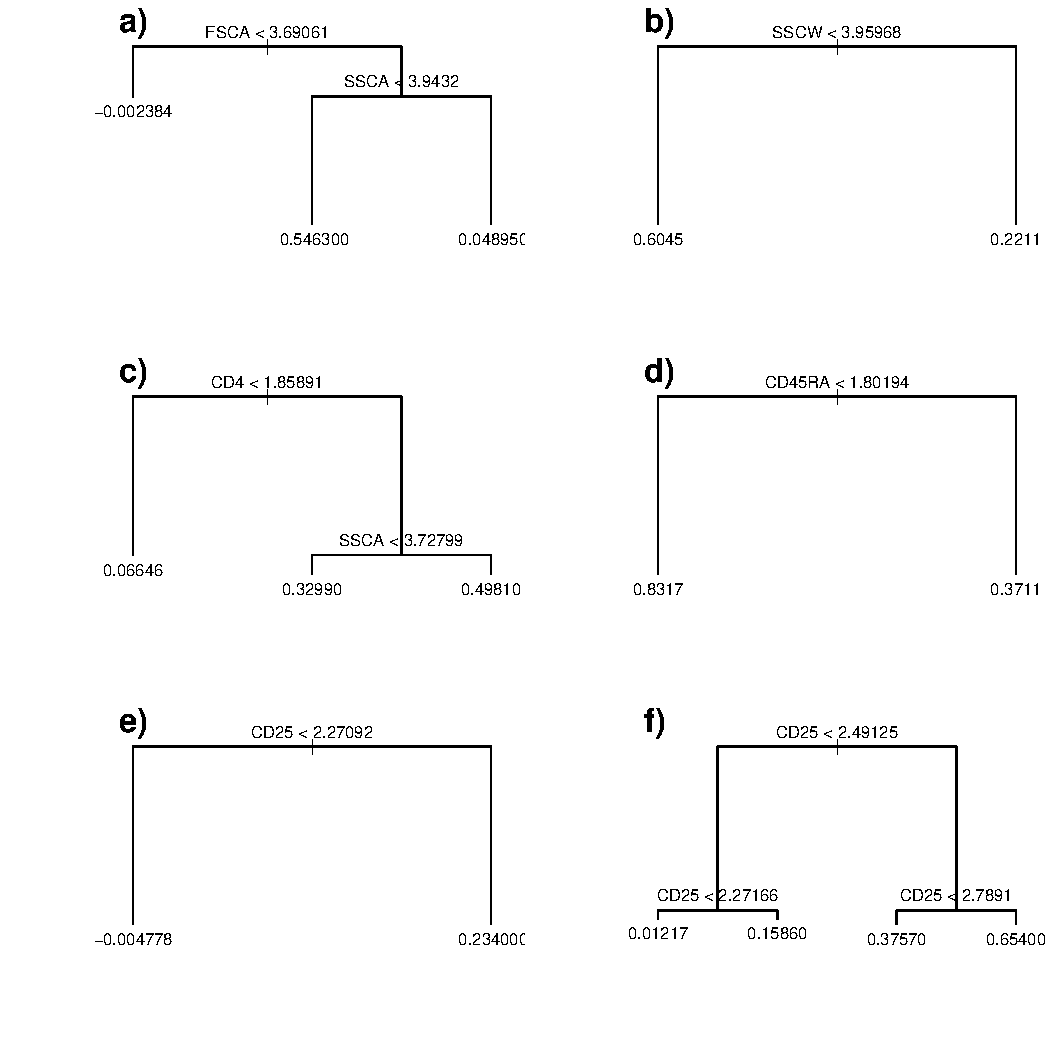
\includegraphics[scale=.4]{figures/tree-CB01494Y_2013-01-29.pdf}
%\mycaption{figure:supervised-cart}
%{ Emulating the manual gating with a regression tree. }
%{
  %For each combination of two markers used in the manual gating, a regression tree is applied to the pSTAT5 response and the relevant split is selected
  %on the marker used in manual gate.
  %The values at the leaf nodes are the expected pSTAT5 response.
  %Note that the tree tends to overdivide the datasets compared to the manual gating since the trees are unpruned.
  %The ellipses are drawn from the mean and covariance of the clustered data.
%}
%
%\end{figure}


\subsection{Identification of low-dose sensitive cells by recursively applying a two component mixture model on pSTAT5}

The CART approach seeks the core marker split point which minimises the deviance of the response variable.
This approach discriminates, based on side and forward scatter, the lymphocytes as the most responsive cluster
when stimulated at the highest 1000 unit dose of proleukin.
Unfortunately, it is not sufficiently sensitive to detect the small proportion of cells which are responsive to lower doses of proleukin.

In order to address this issue, I developed an approach based on the theory that by recursively subsetting responding cells at decreasing doses of proleukin,
it should be possible to identify cells which respond to the lowest proleukin dose.
%As at the highest dose of proleukin, 1000 units, the pSTAT5 distribution appears bimodal, while at lower doses the response peak is less discernable.
%In the ungated sample the majority of cells are non-responsive even at the highest dose.
The algorithm, as illustrated in \Cref{figure:pstat5-rpart}, proceeds by first dividing cells as low responders and high responders on pSTAT5 response at 1000U 
by fitting a two-component \gls{GMM}.
The responder population (in green) is then further divided into low and high by fitting the \gls{GMM} on the pSTAT5 response at 10U.
This process is then repeated in the pSTAT5 response stimulated at the lowest doses of 0.1 units.
Cells which consistently appear in the high group are the most sensitive.
This hierarchical approach draws some similarity to the recursive partitioning using \gls{CART} except that the splitting decision depends only
on applying a two-component \gls{GMM} to the pSTAT5 distribution rather than selecting a core marker value on which to do the split.
Also, at each step, the pSTAT5 at a lower dose is considered to discover cells which respond to the lowest dose of proleukin.
The process is entirely driven by the bimodality of the pSTAT5 distribution.
The clustering on the core markers is only applied right at the end to identify subsets of cells.




Successive univariate clustering on response is not an obvious approach to multivariate data analysis but proves to be useful in identifying potentially interesting cells.
One drawback of this approach is that since the scatter and core markers don't influence the gating, some cleaning of the reported cells is required to eliminate
debris and doublets.

I find that, while many of the cells identified using this approach fall within the CD4 gate,
certain highly-sensitive cells cluster in other subsets \Cref{figure:new-cell-subset}.
Excluding doublets on the basis of side scatter width,
and examining the remainder on other channels these cells appear to be monocytes (from discussion with \contributor{Marcin Pekalski} and \contributor{Tony Cutler}),
although additional markers would be required to better characterise these cells.
%Monocytes are the largest of the leukocytes and are part of the innate immun system
Importantly, these cells would have been missed by manual gating since they are not lymphocytes.
This approach could potentially be extended to identify cells which respond to low doses of proleukin.


\hspace{-2cm}
\begin{figure}[h]
\centering
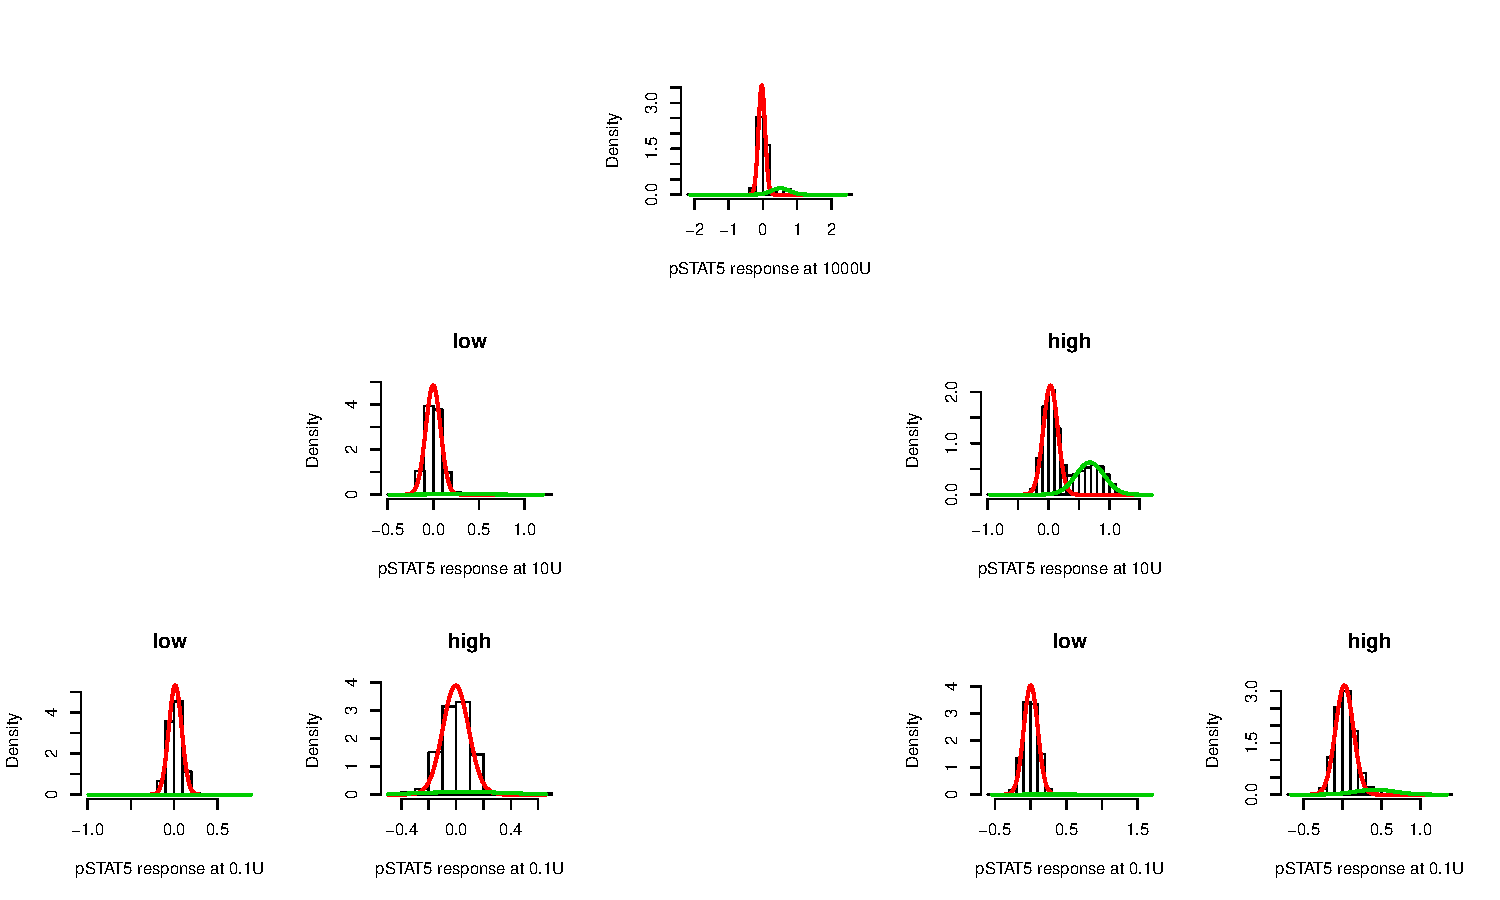
\includegraphics[scale=.5]{IL2/figures/pstat5-rpart.pdf}
\mycaption{figure:pstat5-rpart}
{ Recursive partitioning of pSTAT5 response into low (red) and high (green) populations to identify cells responsive to the lowest dose of proleukin. }
{
In the ungated sample the majority of cells are none responsive even at the highest dose.
Cells are divided as low responders and high responders on pSTAT5 response (i.e baseline subtracted) at 1000U 
within responders further divide on low/high on pSTAT5 response at 10U
repeat on pSTAT5 response at 0.1U
cluster ones which are consistently high, these are the most sensitive cell populations 
}
\end{figure}


\hspace{-2cm}
\begin{figure}[h]
\centering
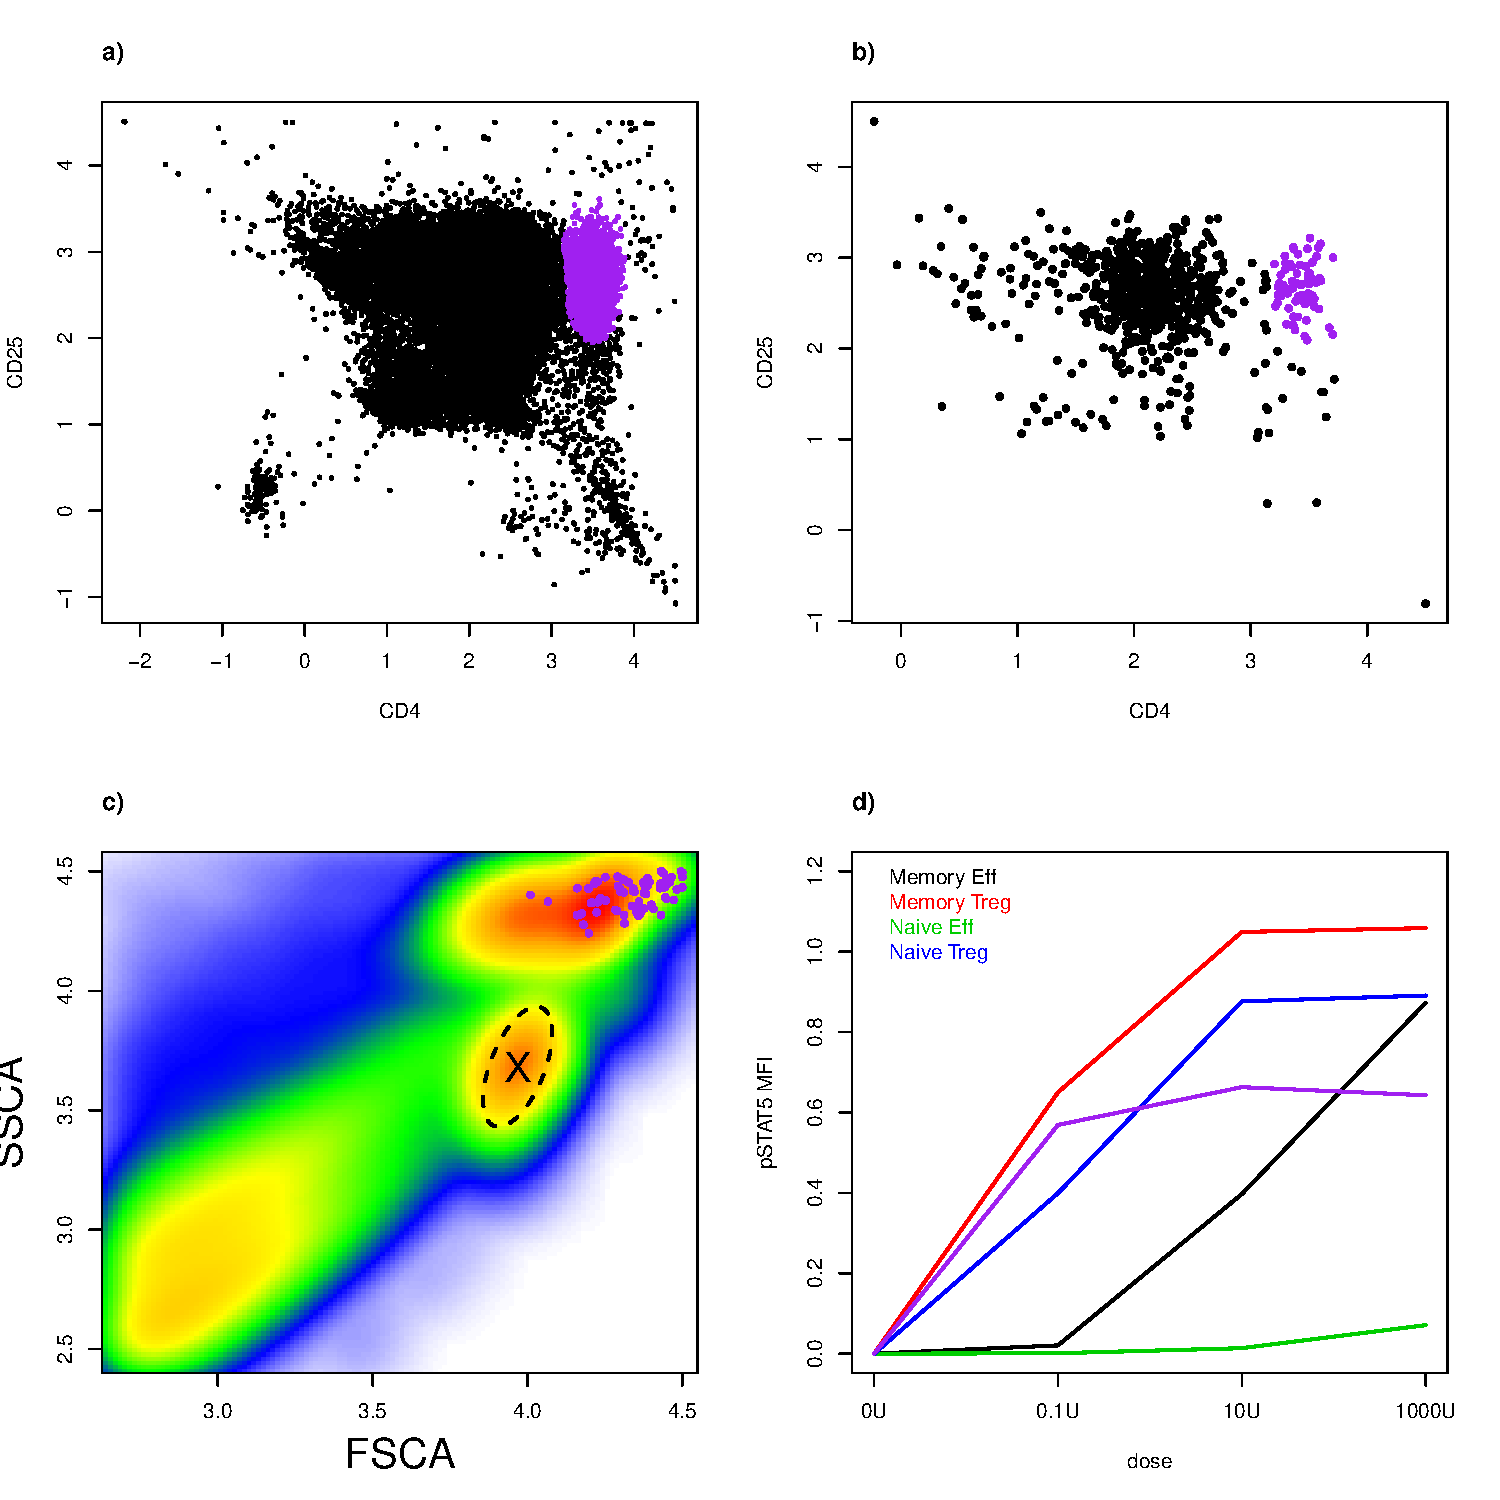
\includegraphics[scale=.5]{figures/new-cell-subset.pdf}
\mycaption{figure:new-cell-subset}
{ Identification of low-dose sensitive non-CD4\positive lymphocyte population through recursive partitioning of pSTAT5 response. }
{
  By pooling all high-responsive cells on CD4 and CD25, we identify a cluster of cells high on CD4 (a).
  This cluster of cells is identifiable in a single sample (b).
  According to forward and side scatter, these cells are unlikely to be lymphocytes, as defined by the dashed lines (c).
  These cells show high-sensitivity to low-doses of proleukin but rapidly reach saturation (d).
  This is probably because they have high resting pSTAT5 levels.
  
}
\end{figure}




\section{Discussion}

\subsection{Comparison with previous studies}
%\subsection{Repeatability of pSTAT5}
%\subsection{Association of pSTAT5 with T1D}

The Long et al study was in a small number of individuals 66 cases and 125 controls and the reproducibility of the phenotypes was not assessed.
\contributor{Tony Cutler}, on the other hand, found that the response of the fluoresence intensity of pSTAT5 to stimulation was poorly reproducible in the various cell subsets
examined.  I attempted to improve on the reproducibility of the fluorescence intensity by using single-cell background correction and peak normalisation.
One reason why the pSTAT5 MFI is not reproducible in memory effector cells is because the pSTAT5 distribution is not unimodal.
In naive and memory regulatory T cells, the pSTAT5 distribution is unimodal but the peak shift on stimulation is not reproducible.
\contributor{Tony Cutler} claims that this is because the titration is too fine and noisy so that there is a lot of uncontrolled variation in the proleukin doses.
This motivated counting the percent of cells whose pSTAT5 fluorescence is greater than the 99th percentile of the pSTAT5 distribution in the unstimulated sample.
Since this phenotype was found to be slightly more reproducible, it was used to test the association with T1D in the four cell subsets, memory, naive, effectors and Tregs.

%They "barcode" multiple samples including 2 controls with a combination of 2 fluorescent dyes,
%pool them and stimulate in one tube with a dose of IL-2 then run through the protocol and then run on the flow.
%The samples are then deconvoluted on the flow by flourescence. I think they then "normalise" on the 2 internal controls.


%No significant associations were found which puts back into question the results of the Long et al study.

Also of concern is that the Long et al dose is too high for the studied cell subsets.
Our dose range is from 0, 0.1, 10 and 1000 U/ml, whereas theirs was 100U/ml 
We find that pSTAT5 Tregs are maximally stimulated by 10 U/ml and near maximum at 0.1U/ml,
which is in contrast to Long et al in which maximum stimulation was not achieved at 100U/ml.
One difference is that Long et al used frozen \gls{PBMC}, while we used fresh blood.
\cite{Dendrou:2009dv} showed that the repetability of a cell phenotype can be compromised with frozen samples
and this difference may explain the difference in response in the two studies.
%We had the same unit measure of IL-2 i.e U/ml.
%They also used Proleukin or equivalent.



%Tony
%I started getting some interesting data with the ND diabetics which in the end flattened to a null result.
%We initiated the LS diabetic study to see 1.
%If we could see the same findings we were initially observing in the ND diabetics and 2.
%Whether there was any relationship between IL-2 sensitivity and duration of disease.
%You could think that some events might only occur close to diagnosis.


%Such cell are of great interest because current clinical trials which administer doses of IL-2 in the hope of increasing T-reg frequency

\subsection{Normalisation of pSTAT5}

Several normalisation methods were attempted to make the pSTAT5 dose-response phenotype more reproducible.
%Of which correcting for resting pSTAT5
However none were able to substantially improve the repeatability.
Unsuprisingly given the small dataset and the poor repeatability, no significant association was detected with dose-response
and disease status.
The conclusion is that this assay is unlikely to be appriopriate for this sort of analyses.


\subsection{ Automatic methods of identifying dose-responsive cell populations }

I have attempted three methods of identifying dose-responsive cell populations.
The main distinction is that the first relies on pooling across doses, while the second and first does nearest neighbour joining to obtain a single sample
containing as many events as the base sample.

The first uses the established spade method which uses density-dependent downsampling to uniformly probe the core marker space.
This idea of uniformising the density has also been explored with probability binning.
With this approach I was able to assess the response at the four proleukin doses.
One drawback of this methods is that each cluster and especially larger clusters in regions of high density, may contain both dose-responsive and none responsive cells,
which could obfuscate the identification of these cells.

The second method I explored was to use the pSTAT5 response to guide the binary recursive partitioning of the core marker space using cart.
Using this approach on side and forward scatter, the lymphocyte population was consistently identified as the most responsive cell population in all samples
stimulated at 1000 units.
However I found that applying this method on all markers across samples would yield different recursive partitioning schemes on different markers.
The alternative to cart which avoids overfitting is random forests.

The third approach I attempted was applied with the objective of identifying highly sensitive dose-responsive cells.
These are cells which would respond at the lowest dose of proleukin.
By recursively splitting the bimodal pSTAT5 distribution in a sample at decreasing doses of proleukin, the hope was to identify cells which respond to low doses of proleukin.
Using this method certain a subset of highly responsive cells was identified which had been lied very close to the lymphocyte gate based on side and forward scatter.
The disadvantage of this approach however is since the core markers do not feature in the identification of cell subsets, there is no garantee that the identified
dose-responsive cells represent a homogeneous subset.  This is why it was necessary to pool across samples in order to 

The methods described in this chapter can be applied to identifying dose-responsive cells in stimulation experiments.
Although spade suggests the mst as a visualisation tool, it is not necessarily the most representative representation of the data since
established cell types do not necessarily cluster in the branches.
Furthermore it can be misleading since the layout is arbitrary and the branching is not always meaningful.
Spade contains an element of stochasticity in its downsampling so that running spade twice on the same data does not give the same tree.
In my opinion, the true value of spade as applied to automatic gating or exploration of the dose-response in these datasets,
lies in the downsampling and agglomerative clustering steps which allow for probing of the entire marker space.
Furthermore, the raw data used to create the mst visualisation can been used to represent the data in a number of ways using established
MDS methods which rely on the distance matrix computation.

Another advantage of the spade approach over the other two described methods is that it does not rely on joining samples on nearest-neighbour.
Since pooling effectively averages the signal across samples it is less sensitive to debris.
Nearest neighbour joining can run into trouble if certain subsets are not present across all samples, as this can lead to mapping to the wrong subset
or certain subsets not beeing represented.
Nearest neighbour is advised if the total number of events varies greatly between samples.
Also if the location of cell subsets differs significantly then this can also lead to joining to the wrong subsets.
One way of assessing whether samples are significanly different is to use probability binning on in the context of spade to identify clusters whose proportion
varies greatly between samples.  Generally when pooling within batches this does not seem to occur, however across batches this is problematic. 


Using these methods in these pbmc samples, it is pretty conclusive that the strongest dose-response comes from the lymphocyte subset.
Although other cell types which carry IL-2 receptors are candidates, the majority of the response appears to lie within the lymphocyte subset.

%A manuscript is in preparation with the intention of submitting to Flow Cytometry Part A








